\documentclass[10pt]{article}
\usepackage{commands}


\begin{document}
%Course webpage: https://phas.ubc.ca/~seme/516/
\begin{tcolorbox}
  \begin{center}
  \begin{Large}
    \textbf{PHYS 516 (Statical Mechanics) Notes} \\
    \vspace{5pt}
  \end{Large}
  \begin{large}
        Rio Weil \\
\vspace{5pt}
    \emph{This document was typeset on \today}
  \end{large}
  \end{center}
\end{tcolorbox}
% Email: gordonws@phas.ubc.ca
% Office: Henn 344
% Webpage: https://phas.ubc.ca/~seme/516/


\begin{center}
  \textbf{Introduction:}

  This is a set of lecture notes taken from UBC's PHYS 516 (Graduate Statistical Mechanics) course, taught by Dr. Gordon Semenoff. The course covers fundamentals of statistical mechanics, phase transitions and critical exponents, $D = 1,2,3$ Ising models, mean field theory, quantum field theory, universality, renormalization, and elementary conformal field theory. If any errors are found in the notes, feel free to email me at \href{mailto:ryoheiweil@phas.ubc.ca}{ryoheiweil@phas.ubc.ca}.
\end{center}
\addtocontents{toc}{\protect\hypertarget{toc}{}}
\tableofcontents

\newpage
\section{Introduction, Statistical Mechanics Review}

\subsection{Overview}
This course centers around critical phenomena and phase transitions (primarily in magnetic systems/the Ising model) - PHYS 403 is a more comprehensive overview of the field, this is more specialized. We will discuss models that are analytically solvable (or almost), some renormalization group methods, some conformal field theory and the conformal bootstrap method.

We will begin with a review of some basic statistical mechanics. In a nutshell, statistical mechanics is the application of probability theory to a physical system - typically, with a large number of degrees of freedom as this is the limit where the application is useful. Perhaps saying probability theory is a bit reaching, though - the probability involved is pretty minimal (lots of counting, not a ton of measure theory). It is worth noting that (much like other fields of physics) there are very few systems that are analytically solvable; most systems require the application of approximate techniques.

\subsection{Canonical Ensemble}
There are various places to begin this discussion; let's start by discussing the canonical ensemble. Let us consider a physical system, which has an array of possible states. Let us assume that it is characterized by energies $E_a$, and the energy can take up one out of a list of possible values $E_1, E_2, E_3, \ldots$. Given the conservation of energy for a closed system, this is a reasonable way to characterize a state (and given one of our goals of doing thermodynamics with our system, this is a useful quantity). Let us not say too much more about the system - other than perhaps the fact that the energy has a lower bound (but not necessarily an upper bound), and that the energies are ordered. Further, for now let us assume that the energies are discrete - this is of course not true in general (there exist systems for which energy is a continuum, and there we will have to use some kind of binning procedure), but let us assume this simplification for now.

So, how do we make the canonical ensemble? We take $\N$ copies of the system, with various energies, so that $\mathcal{E} = \sum_{i=1}^{\N} E_i$ is the total energy. The $\N$ copies of the system are weakly coupled to each other. This means that energy can flow between the systems, but also that (since the coupling is weak) when we calculate the total energy we can neglect the interaction energies between the systems. In other ensembles, other things that are not the energy can be exchanged (e.g. particles in the grand canonical ensemble).

\begin{figure}[htbp]
    \centering
    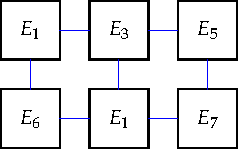
\includegraphics[]{Images/fig-canonicalensemble.pdf}
    
    \caption{Cartoon of the Canonical Ensemble - we consider $\N$ ($= 6$ here) copies of a system, and weakly couple them such that they can exchange energy.}
    \label{fig-canonicalensemble}
\end{figure}

In state of the ensemble is specified by the number of systems with a given energy, i.e. there are $n_1$ systems with energy $E_1$, $n_2$ systems with energy $E_2$, and so on. The total energy is then given by:
\begin{equation}
    \mathcal{E} = \sum_{a} n_a E_a
\end{equation}
and the number of systems in the ensemble is given by:
\begin{equation}
    \N = \sum_a n_a
\end{equation}

\subsection{Fundamental Postulate - Equal a Priori Probability}
To do statistical mechanics, we require a fundamental postulate - namely, an ``equal a priori probability''. This says that every distinct configuration of the ensemble is equally likely, subject to the total energy and number constraints. Physically, this means that the systems in the ensemble in time are flipping around the possible energy states (in a way that the total energy of the ensemble is conserved). The most probable configuration is the state in which the system spends the most time.

There are other versions of this; we can for example divide a system up in space, and then a spatial average will yield the most probable distribution.

What we look for (since the system visits every possible configuration equally) is the configuration which can be made in the most number of ways. And this is really the only probability theory we have to worry about here; counting up the number of ways to yield a given configuration of the ensemble. So, we ask how many ways are there to make the state $(n_1, n_2, \ldots)$? Let us derive this. Starting with the systems with energy $E_1$, we have:
\begin{equation}
    \N(\N-1) \ldots (\N - n_1 + 1)
\end{equation}
ways to have $n_1$ systems with energy $E_1$ (this is obtained by considering there are $\N$ systems to choose to have energy $E_1$, then $\N - 1$ systems, and so on until all $n_1$ systems have been chosen). But this is overcounting because we don't care about the order, so really we require to divide this by $n_1!$:
\begin{equation}
    \frac{\N(\N-1) \ldots (\N - n_1 + 1)}{n_1!}
\end{equation}
and we continue with $n_2, n_3$ and so on until everything is full:
\begin{equation}
    \frac{\N(\N-1) \ldots (\N - n_1 + 1)}{n_1!} \frac{(\N - n_1) \ldots (\N - n_1 - n_2 + 1)}{n_2!} \ldots = \frac{\N!}{n_1!n_2!\ldots}
\end{equation}
So, the most probable state of the system is that for which the above is maximized; in other words, we maximize it subject to $\sum_{a} n_a = \N$ and $\sum_a n_a E_a = \mathcal{E}$. This is a optimization problem with constraints - this may remind you of Lagrange multipliers which you have seen in classical mechanics. There is an apparent difficulty here in the fact that our numbers are discrete, but we'll get around it. To start, let us take the logarithm of the expression; we can maximize the logarithm of it instead of the original expression, and this is legal as the logarithm is monotonic (this is also a common trick done in machine learning and maximum likelihood estimation). The technique of Lagrange multipliers tells us that the expression of our interest is:
\begin{equation}\label{eq-Lagrangemults}
    \ln(\frac{\N!}{n_1!n_2! \ldots}) + \beta\left(\sum_a n_a E_a - \mathcal{E}\right) + \gamma\left(\sum_a n_a - \N\right)
\end{equation}
it would be nice to be able to use calculus techniques to solve this problem; to this end let us work in the regime of large $\N$ such that we can make the continuum approximation. At first this might seem like a poor assumption; after all after we saturate $\mathcal{E}$ all of the $n_a$s past that point better not be large, but instead zero! To get around this we could assume some kind of cutoff to the energies. Of course there is still a decaying tail to the $n_a$s, but these turn out to not be a problem.

In any case, let us suppose that we can approximate $\N$ large. Then, we can apply Stirling's formula:
\begin{equation}\label{eq-Stirling}
    \ln \N! \approx \N\ln \N - \N.
\end{equation}

\subsection{Interlude - Deriving Stirling's Formula}
We start by writing down an integral expression for the factorial:
\begin{equation}
    \N! = \int_0^\infty dx x^\N e^{-x}
\end{equation}
we solve this via a saddle point technique of replacing the integrand with its maximum value; taking the derivative of the integrand and setting it to zero, we have:
\begin{equation}
    \N x^{\N-1}e^{-x} - x^\N e^{-x} = 0
\end{equation}
which is maximized at $x = \N$. so, the approximate value of the factorial is:
\begin{equation}
    \N! \approx \N^\N e^{-\N}
\end{equation}
and taking logarithms we get Eq. \eqref{eq-Stirling}. This technique also gives us a way of considering corrections to Stirling's formula by considering $x$ near $\N$ (the next order corrections to $\ln \N!$ are $O(\log \N)$, for example).

Another quick and dirty way to derive the formula (that doesn't give a nice way to study corrections, but gives us the leading terms that we want). Using the definition of the factorial and laws of logarithms, we have:
\begin{equation}
    \ln \N! = \sum_{j=1}^\N \ln j
\end{equation}
now approximating the sum as an integral:
\begin{equation}
    \ln\N! \approx \int_1^\N dj \ln j = \N\ln\N - \N + 1
\end{equation}
in the large $\N$ limit we may neglect the $+1$, and we (again) obtain Stirling's formula.

\subsection{Deriving the Boltzmann Distribution}
Applying Stirling's Formula, Eq. \eqref{eq-Lagrangemults} becomes:
\begin{equation}
    \N\ln\N - \N - \sum_a(n_a \ln n_a - n_a) + \beta(\sum_a E_a n_a - \mathcal{E}) + \gamma(\sum_a n_a - \N) = \N\left(\sum_a(-\rho_a \ln \rho_a) + \beta(\sum_a \rho_a E_a - U) + \gamma(\sum_a \rho_a - 1)\right)
\end{equation}
where we define $\rho_a = \frac{n_a}{N}$ and the second expression follows by algebra. Now, since $\rho_a$ varies slowly, we may use techniques of calculus and take a derivative of the above expression and set it to zero. The $\rho_a$ equation reads:
\begin{equation}
    -\ln \rho_a - 1 + \beta E_a + \gamma = 0
\end{equation}
we also take derivatives by $\beta, \gamma$ and set them to zero (as we do with the Lagrange multiplier technique):
\begin{equation}
    \sum_a \rho_a E_a = U
\end{equation}
\begin{equation}
    \sum_a \rho_a = 1
\end{equation}
Let us rearrange the first equation, which has solution:
\begin{equation}
    \rho_a = e^{\beta E_a + \gamma - 1}
\end{equation}
we don't solve the second one, but the third one gives us:
\begin{equation}
    \rho_a = \frac{e^{\beta E_a}}{\sum_a e^{\beta E_a}}
\end{equation}
Note that the $e^{\gamma - 1}$ goes away when we solve the third equation. It would have been wise to choose $\beta$ with the other sign to start with. As we have derived things here, things only make sense if $\beta < 0$. We note that we have derived the ever-famous partition function:
\begin{equation}
    Z = \sum_a e^{\beta E_a}
\end{equation}

So, we have solved for the most likely distribution $\rho_a$; this is the known as the ``Boltzmann distribution''. We have not solved explicitly for $\beta$, but the second equation is formally unsolvable, and we will find a nice interpretation for $\beta$ anyway (as the familiar $\beta = -\frac{1}{k_B T}$). 

\subsection{Example: Two-level system}
We really have not done any physics at all here; but, we have completely generically found the most probable distribution. Let us try applying this to a two-level system and see how good our result is. Particles can have two (spin) states, $\uparrow$ and $\downarrow$. Let us assume we have two particles, and let us assume all orientations of the spins have the same energy. We can just enumerate all the states, and characterize the system by the net magnetization $m = \# \uparrow - \# \downarrow$. We have the four states $\uparrow \uparrow$ with $m = 2$, $\downarrow \downarrow$ with $m = -2$, $\uparrow\downarrow$ and $\downarrow \uparrow$ with $m = 0$. Here, the technique of most probable distribution is quite poor - there is a very good probability that the system is actually ferromagnetic (in fact half of the time) even though the most probable distribution is that the system is unmagnetized. However, we are able to see that unmagnetized is the most probable distribution, and in fact this is true for any number of particles.

So, let's consider generically $N$ particles (note - let us assume that $N$ is even so we can avoid frustration; if $N$ is odd then there exists no configuration with zero magnetization). With $N$ particles, the number of states with $n$ spins up (from which we can obtain the magnetization as $m = n - (N - n) = 2n - N$) is $\frac{N!}{n!(N-n)!}$ of $2^n$ total possible states.

If we then plot $\ln \frac{N!}{n!(N-n)!}$ (making the continuum approximation), we find:

\begin{figure}[htbp]
    \centering

    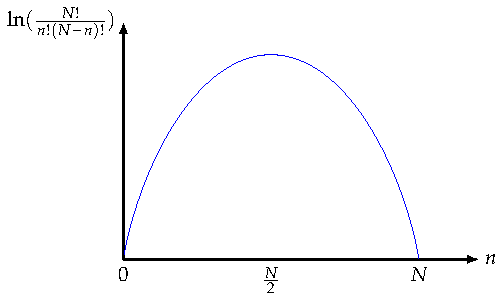
\includegraphics[]{Images/fig-TLSstatecounting.pdf}
    
    \caption{Plot of (continuum approximation) $\ln\frac{N!}{n!(N-n)!}$ as a function of number of spin-up spins $n$. We see the maximum at $n = N/2$ (zero magnetization).}
    \label{fig-TLSstatecounting}
\end{figure}

so indeed the state with $n = N/2$ spins up (and $n = N/2$ spins down) - the state with total magnetization $m = 0$ is the most probable state. It is also valuable to ask what fraction of the total number of states is the most likely distribution. This is simply obtained by taking the number of states with $n = N/2$ and dividing by the total $2^n$:
\begin{equation}
    \frac{N!}{(N/2)!(N/2)!} \frac{1}{2^{n}}
\end{equation}
We find that (using Stirling's formula that):
\begin{equation}
    \ln( \frac{N!}{(N/2)!(N/2)!} \frac{1}{2^{N}}) = 0 + \frac{\ln N}{N}
\end{equation}
so in the $N \to \infty$ limit, $\frac{N!}{(N/2)!(N/2)!} \frac{1}{2^{N}} \approx 1$ to leading order, so the proportion of the most likely distribution to total states of the system is one (with corrections given by the successive terms).
\newpage
\section{Free Energy, Ideal Gas, and the Grand Canonical Ensemble}

\subsection{Thermodynamic Interpretation, Energy, and Free Energy}
Last time, we looked at the canonical ensemble. We derived the most probable distribution:
\begin{equation}
    \rho_a = \frac{e^{-\beta E_a}}{\sum_a e^{-\beta E_a}}
\end{equation}
and found the partition function:
\begin{equation}
    Z = \sum_a e^{-\beta E_a}.
\end{equation}
We argue that this already has a nice thermodynamic interpretation. This comes about if we look at the logarithm of the partition function:
\begin{equation}
    F = -\frac{1}{\beta}\ln Z = -\frac{1}{\beta}\ln \sum_a e^{-\beta E_a}
\end{equation}
Note that if there was only one energy level, then this would immediately just be the energy - in general the energy we calculate as the expectation value:
\begin{equation}
    U = \frac{\sum_a E_a e^{-\beta E_a}}{\sum_a e^{-\beta E_a}}
\end{equation}
How does $F$ relate to $U$? Let us write:
\begin{equation}
    F = U + \left(-\frac{1}{\beta}\ln \sum_a e^{-\beta E_a} - \frac{\sum_a E_a e^{-\beta E_a}}{\sum_a e^{-\beta E_a}}\right)
\end{equation}
Let us call $e^{-\beta E_a} = Z \rho_a$ and write $E_a = -\frac{1}{\beta}\ln Z - \frac{1}{\beta}\ln \rho_a$. Then, rewriting the above expression, we find:
\begin{equation}
    F = U - \frac{1}{\beta}\sum_a \rho_a \ln \rho_a.
\end{equation}
The second term should be familiar to anyone with an information theory background - $S_{VN} = \sum_a \rho_a \ln \rho_a$ is known as the von Neumann entropy. It is the entropy of the distribution - a measure of how little we know about the system when we have the distribution $\rho_a$. It is minimized if one of the $\rho$s is one and the others are zero, as the entropy is zero (then we know exactly what the system is). It is maximized if all of the $\rho$s are constant (because then we know nothing about the system). If we are willing to accept that the von Neumann entropy is equal to the thermal entropy up to a constant:
\begin{equation}
    S = k_B S_{VN}
\end{equation}
where $k_B$ is Boltzmann's constant. Then, we obtain:
\begin{equation}
    F = U - \frac{1}{\beta}\frac{S}{k_B}
\end{equation}
which closely resembles:
\begin{equation}
    F = U - TS. 
\end{equation}
where $T$ is the temperature (if we interpret $\beta = \frac{1}{k_B T}$). This is the familiar thermodynamic expression for the Helmholtz free energy.

This is not the historical order in which things are done - historically the microcanonical viewpoint (due to Boltzmann) came first, but this requires the system to be thermodynamic.

\subsection{Example - System of weakly interacting non-relativistic particles}
Let us assume we have a collection of $N$ weakly interacting non-relativistic particles of mass $m$, which obey the laws of classical mechanics. A state of such a system will just be the specifications of the positions and velocity (or momenta) of all the particles (mathematically, this is because Newton's second law is a second-order ODE so we require two boundary conditions to specify the state). We can write the state as a collection of these values $\set{\v{q}_1, \v{p}_1, \ldots, \v{q}_n, \v{p}_n}$ The energy is then given by the Hamiltonian:
\begin{equation}
    H = \sum_k \frac{\v{p}_k^2}{2m}
\end{equation}
Note we assume that the masses of the particles are the same and all attributes of the particles (other than position or momentum) are identical - note that in the context of classical mechanics this does not make the particles indistinguishable - we can keep track of them. This is in contrast to quantum statistical mechanics, where particles are truly indistinguishable and are either fermions or bosons.

We can construct the partition function for this system:
\begin{equation}
    Z = \int d\v{q}_1 d\v{p}_1 \ldots d\v{q}_n d\v{p}_n e^{-\beta H}
\end{equation}
this looks reasonable, but there are a couple things wrong with this. One problem - $Z$ has dimensions; this is problematic if we want to take functions of it (e.g. logarithms to get the free energy). To deal with this problem, we just divide it by a number that gets rid of the dimensions:
\begin{equation}
    Z = \frac{1}{(2\pi \hbar)^{3N}}\int d\v{q}_1 d\v{p}_1 \ldots d\v{q}_n d\v{p}_n e^{-\beta H}
\end{equation}
$\hbar$ we pretty much pulled out of a hat here, but we require something with the dimensions of angular momentum to place there. Let's now do the integral. Let's assume that our particles move in infinite 3-D Euclidean space; we can then write $\int d\v{q}_i = V$ (the volume) as $H$ does not depend on the positions. Further, all momentum integrals are equivalent, so let us write it as the product of momentum integrals:
\begin{equation}
    Z = \frac{V^N}{(2\pi \hbar)^{3N}}\left(\int dp e^{-\frac{\beta}{2m}\v{p}^2}\right)^{3N}
\end{equation}
We go into polar coordinates to solve this Gaussian integral:
\begin{equation}
    \left(\int dp\right)^{3N} \to \left(\int d^2p\right)^{\frac{3N}{2}} \to \left(\int \frac{d\phi pdp}{2}\right)^{\frac{3N}{2}}
\end{equation}
which yields:
\begin{equation}
    Z = \frac{V^N}{(2\pi \hbar)^{3N}} \left(\frac{2\pi m}{\beta}\right)^{\frac{3N}{2}} = V^N\left(\frac{mk_B T}{2\pi \hbar^2}\right)^{\frac{3N}{2}}
\end{equation}
The Helmholtz free energy is then:
\begin{equation}
    F[T, V, N] = -k_B T N\ln \left[V\left(\frac{mk_B T}{2\pi \hbar^2}\right)^{3/2}\right]
\end{equation}
This system should be truly thermodynamic (as we can take the system to be large), so this should work - we will see in a moment that unfortunately, it does not!

Recall thermodynamic differential relation:
\begin{equation}
    dF = -S dT + \mu dN - P dV
\end{equation}
So the entropy is:
\begin{equation}
    S = \left.-\dpd{F}{T}\right|_{N, V}
\end{equation}
the chemical potential is:
\begin{equation}
    \mu = \left.\dpd{F}{N}\right|_{T, V}
\end{equation}
and the pressure is:
\begin{equation}
    P = \left.-\dpd{F}{V}\right|_{T, N}
\end{equation}
so we can go to town and calculate some quantities. For example
the pressure we can calculate to be:
\begin{equation}
    P = \frac{N k_B T}{V}
\end{equation}
which is the ideal gas law! Big success (the other quantities will not be as successful...)! The chemical potential we can calculate to be:
\begin{equation}
    \mu = -k_B T\ln\left(V\left(\frac{mk_B T}{2\pi \hbar^2}\right)^{3/2}\right)
\end{equation}
The entropy we calculate to be:
\begin{equation}
    S = \frac{3}{2}k_B N + k_B N\ln\left(V\left(\frac{m k_B T}{2\pi \hbar^2}\right)^{3/2}\right)
\end{equation}
We can calculate the energy to be:
\begin{equation}
    U = F + TS = \frac{3}{2}N k_B T
\end{equation}
which is again a beautiful formula (and the correct result). However, we should talk about why the formulas for $\mu, S$ are wrong. They do not have the correct extensivity properties. Concretely, if one considers two identical volumes of ideal gas separated by a partition, removing and re-inserting the partition should be reversible. However, a calculation of the entropy change shows that removing the partition leads to an increase in entropy of $2k_B N \ln 2$; contradiction. So we're a failure. But we're also clever, and can try to fix it. We introduce a factor of $\frac{1}{N!}$ into the partition function. This introduces a factor of $\frac{1}{N}$ into the logarithm in the free energy expression, which ends up correcting things. This was originally a fudge factor fix, but it turns out to be quite deep - namely, we have overcounted the states in the system somehow, and the $\frac{1}{N!}$ corrects for this. This hints to classical mechanics being problematic (quantum statistics fixes this with indistinguishability). 

But let's try taking $Z \to \frac{1}{N!}Z$ (we are exploring what is known as Maxwell-Boltzmann statistics). Then with Stirling's formula:
\begin{equation}
    \ln N! \approx N\ln N - N = \ln \left(\frac{N}{e}\right)^N
\end{equation}
Then the free energy becomes:
\begin{equation}
    F[T, N, V] = -k_B T\ln\left[\frac{eV}{N}\left(\frac{mk_B T}{2\pi \hbar^2}\right)^{3/2}\right]
\end{equation}
and now we see that $F$ has the correct scaling properties so things have been fixed. If we now recalculate quantities, $P, U$ stay the same (as beautiful as they were):
\begin{equation}
    PV = Nk_B T
\end{equation}
\begin{equation}
    \frac{U}{N} = \frac{3}{2}k_B T
\end{equation}

And now the entropy is fixed up as well:
\begin{equation}
    S = \frac{3}{2}k_B N + k_B N\ln\left(\frac{eV}{N}\left(\frac{mk_B T}{2\pi\hbar^2}\right)^{3/2}\right)
\end{equation}
and this is known as the \emph{Sackur-Tetrode equation}.

Before we go on - there are other ensembles we could have used, e.g. the grand canonical ensembles where the subsystems are allowed to exchange particles as well as energy. We need this as this one is the easier one to use when we consider quantum statistics. So in a way, Maxwell-Boltzmann statistics assumes the distribution is completely symmetric in the particles, but it is blind to how the wavefunction changes - if we take the distribution to be $\rho = \psi^\dag \psi$, it assumes that each permutation comes out to be symmetric. But is not actually completely correct as in QM we impose the proper statistics on the wavefunctions, rather than the density.

\subsection{Grand Canonical Ensemble}
The logic follows exactly the same as the Canonical ensemble, with the only difference that we allow for the particle number to change. Suppose a system has $N_a$ particles in state $a$, and energy $E_a$. We define $n_a$ to be the number of systems in the ensemble in state $a$. We have some constraints:
\begin{equation}
    \sum_a n_a = \mathcal{N}
\end{equation}
\begin{equation}
    \sum_a n_a E_a = \mathcal{E} = \mathcal{N}U
\end{equation} 
\begin{equation}
    \sum_a n_a N_a = \mathcal{N}N
\end{equation}
in the above, $U$ is the average energy and $N$ is the average number of particles. This differs from what we had before by one equation. We want to find the most probable distribution; for this the mathematics is exactly the same, just with one more Lagrange multiplier. We maximize:
\begin{equation}
    \ln \frac{\mathcal{N}!}{\prod_a n_a !} + \beta(U\mathcal{N} - \sum_a n_a E_a) + \alpha\left(N\mathcal{N} - \sum_a n_a N_a\right) + \gamma\left(\mathcal{N} - \sum_a n_a\right)
\end{equation}
The argument is basically identical to what we did to calculate $\rho_a$ for the canonical ensemble. We solve the first and last equations for $\rho_a$ and leave the other two unsolved (they will be thermodynamic quantities we can interpret). After the dust settles, we end up with:
\begin{equation}
    \rho_a = \frac{e^{-\beta E_a - \alpha N_a}}{\sum_a e^{-\beta E_a - \alpha N_a}}
\end{equation}
Our grand canonical partition function is:
\begin{equation}
    \mathcal{Z} = \sum_a e^{-\beta E_a - \alpha N_a}
\end{equation}
If we identify:
\begin{equation}
    \Phi = -k_B T \ln \mathcal{Z}
\end{equation}
with the grand canonical free energy, and go through a similar procedure of identifying the Von Neumann entropy with the thermodynamic entropy (and an identification to relate $\alpha$ with the chemical potential), we obtain:
\begin{equation}
    \beta = -\frac{1}{k_B T}, \quad \alpha = -\frac{\mu}{k_B T}.
\end{equation}
The grand canonical free energy now no longer depends on the number of particles, but on the chemical potential. It is however related to the Helmholtz free energy via a Legendre transform:
\begin{equation}
    \Phi[T, \mu, V] = F - \mu \mathcal{N}
\end{equation}
If we did things correctly, working with the grand canonical free energy vs. the Helmholtz free energy should yield the same answers. If we recall the canonical partition function for the weakly interacting gas, we had a dependence on the particle number $N$ (note - NOT the average number of particles in the systems of the ensemble, but here really the number of particles in the ideal gas. Sorry for the overload of notation). We can sum over $N$ to get the grand canonical partition function. We can then go through and see if we obtain the same results (and we will). We had:
\begin{equation}
    Z[T, N, V] = \frac{1}{N!}V^N\left(\frac{mk_B T}{2\pi \hbar^2}\right)^{\frac{3N}{2}}
\end{equation}
note the inclusion of the $\frac{1}{N!}$ factor so things end up correct. The grand canonical partition function is then:
\begin{equation}
    \mathcal{Z}[T, \mu, V] = \sum_N e^{\frac{\mu}{k_B T}N}Z[T, N, V]
\end{equation}
this is an easy sum because its just $\sum_N \frac{1}{N!}x^N$; hopefully this is familiar as just an exponential:
\begin{equation}
    \mathcal{Z}[T, \mu, V] = e^{V\left(\frac{mk_B T}{2\pi \hbar^2}\right)^{3/2}e^{\frac{\mu}{k_B T}}}
\end{equation}
so our prediction for the grand canonical free energy is:
\begin{equation}
    \Phi = -k_B T \ln \mathcal{Z} = -k_B TV\left(\frac{mk_B T}{2\pi \hbar^2}\right)^{3/2}e^{\frac{\mu}{k_B T}}
\end{equation}
and we can go through the song and dance to obtain the quantities that we solved for using the canonical ensemble.
\newpage
\section{Microcanonical Ensemble, Quantum Statistical Mechanics}
We have spent two lectures discussing the canonical ensemble and grand canonical ensemble - in this setting we have discussed the classical perfect gas. We have one more to discuss; the microcanonical ensemble.

\subsection{Review of the Canonical Ensemble}
The canonical ensemble is a way to find the likelihood that a system is in a particular state; we found the most likely distribution:
\begin{equation}
    \rho_a = \frac{e^{-\beta E_a}}{\sum_a e^{-\beta E_a}}
\end{equation}
with $\beta = \frac{1}{k_B T}$. In deriving this we made some assumptions; for example the fact that the system was able to visit different energy states (this may not be true, e.g., if the system obeys some conservation law). In the setting of the perfect gas, we assumed that the particles were weakly interacting so they could exchange energy and visit different energy states (but weakly so we did not have to consider the interaction very carefully) - if the particles were completely free, they could not change their state (the momenta of all the particles would be fixed). We explored this distribution in the context of an ensemble of two-level systems; for two spins, we found that this was only a good description $\sim 50\%$ of the time, but as we increase $N$ this estimate gets better and better.

\subsection{Microcanonical Ensemble}
The accuracy of the canonical ensemble only depended on the size of the ensemble - if something is not accurate enough, just look at a larger system. Essentially, a given subsystem sees the rest of the system as a heat bath/reservoir, and the estimate will get better as we increase the size of the heat bath. But we might ask - how well is the system described if we assume the system takes the most likely state? Roughly, the system takes the state such that $E^\nu e^{-\beta E}$ is maximized (those with a condensed matter background will be familiar with this sort of expression; the Boltzmann distribution times the density of states).

Concretely, we say:
\begin{equation}
    \rho_a = \begin{cases}
        1 & a: E_a = U
        \\ 0 & \text{otherwise}
    \end{cases}
\end{equation}
This looks extremely crude; it doesn't always work (e.g. the system needs to be highly degenerate) but for most normal things, it does. Let's reason out why. We consider the heat capacity:
\begin{equation}
    C = \left.\dpd{U}{T}\right|_{\ldots} \sim V c
\end{equation}
where $C$ (the total heat capacity) scales with volume (times the per-volume heat capacity/specific heat capacity $c$).

In the canonical approach, $U$ is the average of the energy:
\begin{equation}
    U = \sum_a\frac{ E_a e^{-\beta E_a}}{\sum_a e^{-\beta E_a}} = \avg{E}
\end{equation}
We can write the heat capacity as:
\begin{equation}
    C = \dpd{U}{T} = \frac{1}{k_B T^2}\Delta U^2
\end{equation}
where:
\begin{equation}
    \Delta U^2 = \sum_a \frac{E_a^2e^{-\beta E_a}}{\sum_a e^{-\beta E_a}} - \left(\frac{\sum_a E_a e^{-\beta E_a}}{\sum_a e^{-\beta E_a}}\right)^2 = \avg{E^2} - \avg{E}^2
\end{equation}
i.e. the variance in $E$. Note that both $C$ (and so $\Delta U^2$) and $U$ scale with the volume of the system. Now, if we consider the variance of the energy:
\begin{equation}
    \sqrt{\frac{\Delta U^2}{U^2}} \sim \frac{\sqrt{C}}{V} \sim \frac{1}{\sqrt{V}}
\end{equation}
so as we take $V \to \infty$, the variance in the energy becomes tiny. So the conclusion is that:
\begin{equation}
    \rho_a = \begin{cases}
        \frac{1}{D_a} & E_a = U
        \\ 0 & E_a \neq U
    \end{cases}
\end{equation}
(where $D_a$ is the degeneracy of $E_a$), is a reasonable distribution for (large) systems. 

Note that this can be a useful approach for classical statistical mechanics (for quantum statistical mechanics, the grand canonical ensemble is the best approach). We now have Boltzmann's formula\footnote{Carved on his headstone!} for the entropy in terms of the degeneracy of states:
\begin{equation}
    S = k_B \ln W
\end{equation}
where $W = D_a$. In Boltzmann's work, $W$ was known as the number of ways of making the system with energy $U$ (QM, and hence degeneracy, was not conceptualized at the time). This pre-dates Gibbs, and ensembles - it was a fantastic guess by Boltzmann, though it was not believed by the time.

\subsection{Ideal Gas - Microcanonical Ensemble Lens}
What we need to find is $W$, which in a sense is the partition function in this context. It depends on $U$ (and other quantities), and we obtain it by integrating $\delta(U - \sum_a \frac{\v{p}_a^2}{2m})$ over all possible positions and momenta:
\begin{equation}
    W[U] = \int d\v{q}_1d\v{p}_1 \ldots d\v{q}_Nd\v{p}_N \delta(U - \sum_a \frac{\v{p}_a^2}{2m}).
\end{equation}
There are a couple problems with this formula, one is namely the dimensionality (we want to plug this into a logarithm, so it must be dimensionless). Part of this is the same story as before; we add a phase space volume (fudge factor) of $\frac{1}{(2\pi\hbar)^{3N}}$ to cancel out the dimensions from the integral:
\begin{equation}
    W[U] = \int \frac{d\v{q}_1d\v{p}_1 \ldots d\v{q}_Nd\v{p}_N}{(2\pi\hbar)^{3N}} \delta(U - \sum_a \frac{\v{p}_a^2}{2m})
\end{equation}
Further, we need to cancel out the inverse energy that comes from the dirac delta function, so we add a $\delta U$ factor:
\begin{equation}
    W[U] = \int \frac{d\v{q}_1d\v{p}_1 \ldots d\v{q}_Nd\v{p}_N}{(2\pi\hbar)^{3N}} \delta U\delta(U - \sum_a \frac{\v{p}_a^2}{2m})
\end{equation} 
visually, one can imagine adding a sort of ``thickness'' of a shell of energy in phase space to the integral. This should go away whenever we start to do thermodynamics, though. Furthermore, we are overcounting states here again; so let us add a factor of $\frac{1}{N!}$ to compensate:
\begin{equation}
    W[U] = \frac{1}{N!}\int \frac{d\v{q}_1d\v{p}_1 \ldots d\v{q}_Nd\v{p}_N}{(2\pi\hbar)^{3N}} \delta U\delta(U - \sum_a \frac{\v{p}_a^2}{2m})
\end{equation}
The $\frac{1}{N!}\frac{1}{(2\pi\hbar)^{3N}}$ part of this is quantum, the rest is classical. Now, let's evaluate this. The position integrals are trivial; nothing in the integrand depends on volume, so we just get a factor of $V^N$. For the momentum integrals, we do a rescaling of the dirac delta function and then evaluate it, and also include the unit sphere factor in $3N$-dimensional Euclidean space:
\begin{equation}
    W[U] = \frac{1}{N!}V^N \frac{1}{(2\pi \hbar)^{3N}}\frac{\delta U}{U}(2mU)^{\frac{3N}{2}}\frac{2\pi^{3N/2}}{\Gamma(\frac{3N}{2})}
\end{equation}
Now, recall Stirling's formula $\ln N! = N\ln N - N$. The Gamma function is basically the factorial function, so $\ln \Gamma(x + 1) = x\ln x - x + \ldots$ (up to terms of order $O(\ln x)$). With this, we can clean up our expression for $W$:
\begin{equation}
    W[U, V, N] = \left(\frac{eV}{N}\left(\frac{2e}{3}\frac{mU/N}{2\pi \hbar^2}\right)^{3/2}\right)^{N}\frac{\delta U}{U}
\end{equation}
To get the entropy, a la Boltzmann we take the logarithm of this and then multiply by the Boltzmann constant:
\begin{equation}
    S[U, V, N] = k_B N\ln\left(\frac{V}{N}\left(\frac{\frac{2}{3}mU/N}{2\pi\hbar^2}\right)^{3/2}\right) + \frac{5}{2}k_B N
\end{equation}
for $N$ large, $\ln\frac{\delta U}{U}$ is of order $\ln N$ (not order $N$) so we can neglect it. This is now our thermodynamic entropy, and from it we can derive the thermodynamic quantities that we are interested in. For example the (inverse) temperature is given by:
\begin{equation}
    \frac{1}{T} = \left. \dpd{S}{U}\right|_{V, N}
\end{equation}
from which we can derive:
\begin{equation}
    \frac{1}{T} = \frac{3}{2}Nk_B \frac{1}{U}
\end{equation}
and so:
\begin{equation}
    U = \frac{3}{2}Nk_B T
\end{equation}
which is precisely the equipartition of energy formula for an ideal gas. We can proceed similarly with the pressure, and find the ideal gas law:
\begin{equation}
    PV = Nk_B T
\end{equation}
and all the other nice formulas we derived before. So, this appears to be an equally as valid approach.

So, we've now covered three approaches; if we were to study ideal gases forever, we'd be pretty happy with this results. Particularly at higher temperatures/higher energy, this classical treatment works very well. Note that (after the last 30 minutes of lecture here) we will just use the canonical ensemble to look at Ising systems, and work in the classical regime where we set $\hbar = 0$ (though we will see that quantum field theories emerge in this setting... stay tuned). But for fun, let us quantize this theory, here.

\subsection{Quantum Ideal Gas}
Why is Maxwell-Boltzmann statistics not quite right? It is because in QM, states are described by the wavefunction $\psi(\v{q}_1, \ldots \v{q}_n, t)$, but probabilities are described by $\abs{\psi}^2$. A discussion of identical particles tells us that if we permute the position/particle labels, we get a state with the same energy. Nature tells us that there are only two\footnote{well, there are exotic quasiparticles like anyons... but we leave that to another course} types of statistics possible; the wavefunction is totally symmetric in its labels for bosons and anti-symmetric for fermions. But Maxwell-Boltzmann statistics tells us that the probability is symmetric in the labels, which is not quite right (not really describing either bosons or fermions correctly).

Let us now count a system of (bosonic or fermionic) particles assuming we have a set of single-particle states that the particles can occupy. For bosons an arbitrary number of particles can fill a given state, for fermions this is forbidden (Pauli exclusion principle). Let's say a particle has energy $\e_i$. We now count like physicists; count how many states we have for a few particles, and extrapolate. We take the grand canonical point of view where the system is open and can have any number of particles. We assign to each energy a Boltzmann weight. This sounds complicated, but it will turn out to be pretty easy.

In the case where we have no particles (the vaccum) we have only one possible state, so $\mathcal{Z}_{B}$ and $\mathcal{Z}_{F}$ both start with a 1:
\begin{equation}
    \mathcal{Z}_{B} = 1 + \ldots, \quad \mathcal{Z}_{F} = 1 + \ldots
\end{equation}
if we now have a one particle system, we obtain the single particle term $\sum_i e^{-\beta \mu}e^{-\beta \e_i}$ (with the sum taking care of all possible energies that the particle could have). For a single particle, the bosons and fermion partition functions look the same:
\begin{equation}
    \mathcal{Z}_{B} = 1 + \sum_i e^{\beta \mu}e^{-\beta \e_i} + \ldots, \quad \mathcal{Z}_{F} = 1 + \sum_i e^{\beta \mu}e^{-\beta \e_i} + \ldots
\end{equation}
Now for two particles, the two partition functions start to look different. For fermions, we have $e^{2\beta\mu}\sum_{i < j} e^{-\beta(\e_i + \e_j)}$ (noting that the two particles cannot occupy the same energy):
\begin{equation}
    \mathcal{Z}_F = 1 + \sum_i e^{\beta \mu}e^{-\beta \e_i} + e^{\beta\mu 2}\sum_{i < j} e^{-\beta(\e_i + \e_j)} + \ldots
\end{equation}
for bosons, the two particles can be in the same state, so:
\begin{equation}
    \mathcal{Z}_B = 1 + \sum_i e^{\beta\mu}e^{-\beta \e_i} + e^{2\beta\mu}\left(\sum_{i < j}e^{-\beta(\e_i + \e_j)} + \sum_i e^{-2\beta\e_i}\right) + \ldots
\end{equation}
If we continue in this fashion, we obtain:
\begin{equation}
    \mathcal{Z}_F = \prod_i\left(1 + e^{\beta \mu}e^{-\beta \e_i}\right)
\end{equation}
\begin{equation}
    \mathcal{Z}_B = \prod_i \frac{1}{1 - e^{\beta\mu}e^{-\beta\e_i}}
\end{equation}
Recalling the grand canonical free energy formula:
\begin{equation}
    \Phi[T, \mu] = -k_B T\ln \mathcal{Z} 
\end{equation}
we find for bosons:
\begin{equation}
    \Phi_B[T, \mu] = k_B T\sum_i \ln(1 - e^{\beta\mu}e^{\beta\e_i})
\end{equation}
and for fermions:
\begin{equation}
    \Phi_F[T, \mu] = k_B T\sum_i \ln(1 + e^{\beta\mu}e^{-\beta\e_i})
\end{equation}
having obtained these, we can go ahead and do thermodynamics.

For free fermions/bosons, we have $\e = \frac{\v{p}^2}{2m} = \frac{\hbar^2\v{k}^2}{2m}$. We can then replace the sums in the continuum approximation $\sum_i = V \int \frac{d^3k}{(2\pi)^3}$ and although these will not be solvable analytically we can obtain an approximate result by expanding. It is of interest to note that we can compare the results we get out of doing this with the previous derivation with Maxwell-Boltzmann statistics, and we find that for either 1 particle or in the high temperature limit things will agree. You will get to explore some of these limits in the first assignment.
\newpage
\section{Introduction to the Ising Model}
We have now done a quick (and likely wholly inadequate) review of basic statistical mechanics. From here, we will begin to study phase transitions. We will study on a simple type of phase transition (with some side comments about others) - this is because there is a lot to be learned just by considering this simple example of magnetic/Ising systems. Most of the action here happened in the 1980s (so we aren't learning anything extremely new here) but this is just how physics classes go (but we will discuss the conformal bootstrap at the end of the course, which is something invented this century).

The Ising model was initially studied and solved in one dimension, where there are no phase transitions; it was then initially erroneously concluded that there are no phase transitions in any dimension. Later on it was solved exactly in two dimensions, where it was shown that there was a second order phase transition. This then became the standard model system to consider in the study of phase transitions. Through our study of this system, there is a huge amount of theoretical physics that are seeded by it (e.g. QFT). Even more than that, the language of these fields has largely inspired by the Ising model.

\subsection{The Hamiltonian}
We will use the canonical ensemble to study the Ising model. This is a physical model, so there is a Hamiltonian $H$ which describes the energy of a configuration, and a density:
\begin{equation}
    \rho = e^{-H/k_B T}{Z}
\end{equation} 
with $Z$ the partition function:
\begin{equation}
    Z = \sum_{\text{states}}e^{-H/k_B T}.
\end{equation}
We have the thermodynamic quantity of the Helmholtz free energy:
\begin{equation}
    F = -k_B T \ln Z.
\end{equation}
These are the very general statistical mechanical ingredients. Let's talk about the model itself. It is a model of a magnetic system in one dimension, composed of a number of spins arranged on a lattice. If the spins like to align with each other, then we have a ferromagnetic material, if the spins like to anti-align per-site then we have a antiferromagnet.

How do we describe these spins? We can describe a spin at point $x$ by:
\begin{equation}
    \sigma_x = \begin{cases}
        +1 \\ -1
    \end{cases}
\end{equation}
i.e. a spin at position $x$ which either points up or down. $x$ lives on a lattice; a 2-D lattice is sketched as an example below:

\begin{figure}[htbp]
    \centering
    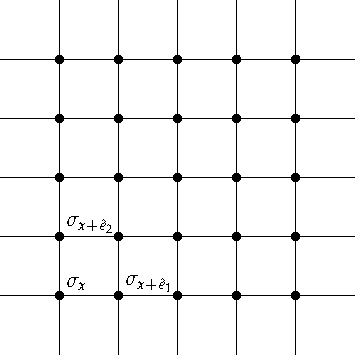
\includegraphics[]{Images/fig-2DIsing.pdf}
    
    \caption{2D Ising model on a square lattice. The spins sit on the nodes/crossings of the lattice, with interaction between neighbouring spins ($\mu = \pm \hat{e}_1, \pm \hat{e}_2$).}
    \label{fig-2DIsing}
\end{figure}

Typically we work in the thermodynamic limit where the lattice is very large (in this limit the boundary conditions should not be important to understand the physics, but this is something we can check). Writing down the Hamiltonian, we have:
\begin{equation}
    H_{interaction} = -J \sum_{x, \mu}\sigma_{x}\sigma_{x+\mu}
\end{equation}
Where $\mu$ runs over the vectors that point to the nearest neighbours of $x$ (so $x + \mu$ runs over the nearest neighbours of $x$). We will not concern ourselves too much with the lattice constant (we can just set it to one). Note that $\sigma_x\sigma_{x+\mu}$ is minimized if the two spins align, (as then $\sigma_x\sigma_{x+\mu}$ is positive and hence the negative sign out front gives the term a negative contribution). We can change the nearest neighbours assumption to include next nearest neighbours, infinite range etc. (and we can also change the behaviour of the interactions) but realistic interactions are short range so for now nearest neighbours is good to consider.

This is almost the Ising model; we can also add a coupling term to an external magnetic field:
\begin{equation}
    H_{B} = -B\sum_x \sigma_x
\end{equation}
where the spins will want to align with $B$ so as to lower the energy. So the Ising Hamiltonian is:
\begin{equation}
    H = H_{interaction} + H_{B} = -J \sum_{x, \mu}\sigma_{x}\sigma_{x+\mu} - B\sum_x \sigma_x.
\end{equation}
This simple two-parameter ($J, B$) model is already quite interesting. From it we will learn about universality - phase transitions tend to be the same for a large number of microsystems, e.g. the critical behavior for the Ising model and for liquid gas phase transition is the same. So this is why we can get away with studying something so simple.

\subsection{Analyzing the Ising Model - Phase Diagram Boundaries}
What we would like to compute is the partition function:
\begin{equation}
    Z = \sum_{\text{spins}}e^{-H/k_B T}
\end{equation}
and we would then like to calculate the free energy $F$, which is a function of the temperature $T$, the field $B$, and the number $N$:
\begin{equation}
F[T, B, N] = -k_B T \ln Z
\end{equation}
if we can find $F$, we can get all sorts of physical quantities, e.g. magnetization, susceptibility etc. For example we have the magnetization (average sum over all spins):
\begin{equation}\label{eq-magnetization}
    M = \left.-\dpd{F}{B}\right|_{N, T} = \frac{\sum_{\text{spins}}(\sum_x \sigma_x)e^{-H/k_B T}}{Z}
\end{equation}

As mentioned previously, we will assume that $N \to \infty$ (thermodynamic limit). What is left in our free energy is $T$ and $B$. So, we can draw a phase diagram:

\begin{figure}[htbp]
    \centering
    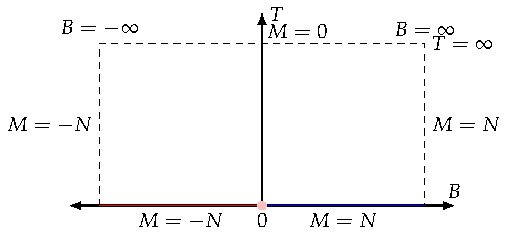
\includegraphics{Images/fig-Isingphasediagramboundaries.pdf}
    
    \caption{Phase Diagram Boundaries for the Ising Model, plotting temperature $T$ and magnetization $M$. As $B = \pm \infty$, the spins want to align all upwards ($M = N$)/downwards ($M = -N$) respectively. As $T \to \infty$, all configurations are equally likely and so $M = 0$. At $T = 0$, all spins aligning minimizes the energy and so for $B < 0$ we have $M = -N$ and for $B > 0$ we have $M = N$. At $T = 0, B = 0$ there is a first order phase transition.}
    \label{fig-Isingphasediagramboundaries}
\end{figure}

Note that as $T \to \infty$, we would first notice that our lab had burned down, but before that we would also notice that our material is no longer a ferromagnetic; it is a paramagnet with $M = 0$. We can see this from our expression for $M$ in Eq. \eqref{eq-magnetization}, where if $T \to \infty$ then $e^{-H/k_B T} = 1$ and so the up and down spins have equal weight, so the net summation comes out to zero.

At $B = \pm \infty$, we have $M \neq 0$. Specifically, if $M = \infty$ then all the spins want to align upwards so $M = N$ and if $M = -\infty$ then the spins want to align downwards so $M = -N$. As the temperature goes to zero, we are interested in the lowest energy state of the Hamiltonian. As all the spins are aligned, this minimizes the energy so actually we find $M = -N$ for all $B < 0, T = 0$ and $M = N$ for all $B > 0, T = 0$. What happens then at $B = 0$? We have a phase transitions between the two domains. We have a first order phase transition there where the magnetization completely flips.

What does the order of the phase transition mean? It refers to the number of the derivatives we can take of the free energy before the derivative does not exist. Here (at $T = 0$), $M = \text{sign}(B) N$, and the derivative of this does not exist at $B = 0$; so the first derivative of $F$ exists but the second one does not, so it is a first order phase transition. This comes from the Landau classification of phase transitions. This is not the full story; we have discovered many topological phases in recent times, and it could be argued that the classification of phases is not yet complete. If we integrate, at $T = 0$ we find $F = J\abs{B}$; this is continuous but not differentiable so the phase transition is first order.

\begin{figure}[htbp]
    \centering
    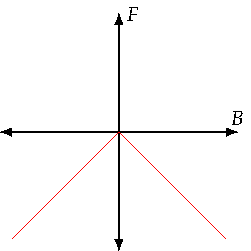
\includegraphics{Images/fig-FT0Ising.pdf}
    
    \caption{Plot of $F$ at $T = 0$ as a function of $B$. The free energy is continuous but not differentiable, and hence there is a first-order phase transition at $B = 0$. The slope of the free energy is $-J/J$.}
    \label{fig-FT0Ising}
\end{figure}

\subsection{Analyzing the Ising Model - $B = 0$ and Spontaneous Symmetry Breaking}
The line of $B = 0$ is interest. This is because the Hamiltonian has more symmetry in this case; namely the symmetry of flipping every $\sigma_x \leftrightarrow -\sigma_x$, or a $\mathbb{Z}_2$ symmetry (which can be represented, e.g. as $\set{1, -1}$ with multiplication). The magnetic field breaks this symmetry.

Note that if we are at some point in the right half of the phase diagram and we do a $\mathbb{Z}_2$ transformation, we map to the point on the other (left) side of the phase diagram (so on the $B = 0$ axis, we do not move at all!) Note however we cannot use symmetry to conclude that $M = 0$ at $B, T = 0$; as the magnetic moment here is dependent on the prior history of the system (how was this critical point reached). So we have some strange behaviour here; at this point, the Hamiltonian has $\mathbb{Z}_2$ symmetry but the actual state of the system does not inherit this symmetry; the system chooses one of the totally magnetized states depending on the prior history. This is known as \emph{spontaneous symmetry breaking}.

Now we can ask; if we go up the $B = 0$ axis (by turning on the temperature) from the $B, T = 0$ point, what happens? Does the symmetry remain broken? In the 1-D Ising model, there is a phase transition where the symmetry is unbroken; the magnetization goes back to $M = 0$. We will show that this comes about through solving the model. In higher dimensions, we cannot exclude the possibility that $M \neq 0$ persists for a while even as we turn up $T$; for example it might be possible that $M$ decays up to some point after hitting zero. We then have a discontinuity in the phase diagram partially along the $T = 0$ axis. We have a line of first order phase transitions, and it ends at some point in a second order phase transition. Unlike the boundaries of the diagrams, we have not really justified this statement; we will have to return to its proof later. 

\begin{figure}[htbp]
    \centering
    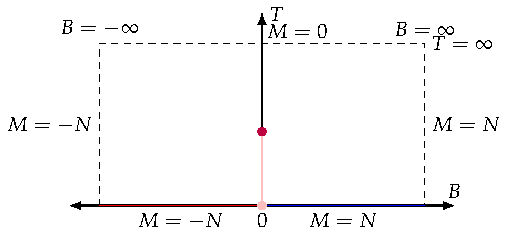
\includegraphics{Images/fig-IsingphasediagramB0.pdf}
    \caption{For dimensions larger than 1, $M \neq 0$ persists at $B = 0$ even as the temperature is tuned up. This results in a ``first order phase transition line'' partway up the $B = 0$ axis, culminating in a second order phase transition point.}
    \label{fig-IsingphasediagramB0}
\end{figure}

It is difficult to study the phase transitions in generality, so we will (later) focus our attention to the point around the second order phase transition. Specifically, things are complicated by the magnetic field, so we will study a neighbourhood of the second order phase transition that lies on the $B = 0$ axis.

We will be able to study the 1-D model in full generality, but this is not very interesting as the ``phase transition line'' we see above will get shrunk to a point. The 2-D model has been solved but only at $B = 0$. 

\subsection{Solving the 1-D model}
One of the slightly unsatisfying things about the study of this system is that the models in different dimensions have different ad-hoc ways of solving them analytically. When we start to look at approximations, we will see a unifying formalism (e.g. renormalization group).

We consider the 1-D Ising model, which is just a chain of classical spins. 

\begin{figure}[htbp]
    \centering
    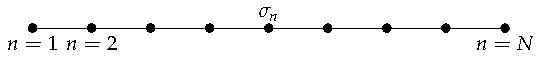
\includegraphics{Images/fig-1DIsing.pdf}
    \caption{Cartoon of 1D Ising model (pictured with $N = 9$ spins). The spin at site $n$ is denoted $\sigma_n$.}
    \label{fig-1DIsing}
\end{figure}

The Hamiltonian takes the form:
\begin{equation}
    H = -H\sum_{n=1}^{N-1}\sigma_n \sigma_{n+1} - B\sum_n \sigma_n
\end{equation}
The route to the solution here is just a brute-force calculation of the partition function:
\begin{equation}
    Z = \sum_{\sigma_1 = \pm 1, \ldots, \sigma_n = \pm 1} e^{\frac{J}{k_B T}\sum_n \sigma_n \sigma_{n+1} - \frac{B}{k_B T}\sum_{n}\sigma_n}
\end{equation}
we rewrite this as an extended multiplication:
\begin{equation}
    Z = \sum_{\sigma_1 = \pm 1} \sum_{\sigma_2 = \pm 1} \ldots \sum_{\sigma_n = \pm 1}e^{-\frac{B}{2k_B T}\sigma_1}\left[e^{\frac{J}{k_B T}\sigma_1 \sigma_2 - \frac{B}{2k_B T}(\sigma_1 + \sigma_2)}\right]\left[e^{\frac{J}{k_B T}\sigma_2 \sigma_3 - \frac{B}{2k_B T}(\sigma_2 + \sigma_3)}\right] \ldots \left[e^{\frac{J}{k_B T}\sigma_{N-1} \sigma_N - \frac{B}{2k_B T}(\sigma_{N-1} + \sigma_N)}\right]e^{-\frac{\beta}{2k_B T}\sigma_N}
\end{equation}
Why would we do this? Because we can take the objects inside the square brackets and call it a 2x2 matrix $T_{ab}$ (with elements that depend on whether the spins are up or down):
\begin{equation}
    T_{ab} = e^{\frac{J}{k_B T}\sigma_a \sigma_b - \frac{B}{2k_B T}(\sigma_a + \sigma_b)}
\end{equation}
where $T_{11}$ has $\sigma_a = \sigma_b = 1$, $T_{22}$ has $\sigma_a = \sigma_b = -1$ and so on. Explicitly:
\begin{equation}
    T_{ab} = \m{e^{\frac{J-B}{k_B T}} & e^{-\frac{J}{k_B T}} \\ e^{-\frac{J}{k_B T}} & e^{\frac{J + B}{k_B T}}}
\end{equation}
We can then write the partition function as:
\begin{equation}
    Z = \sum_{\sigma_1 = \pm 1}\sum{\sigma_N = \pm 1} e^{-\frac{B}{2k_B T}\sigma_1}(T^{N-1})_{\sigma_1\sigma_N} e^{-\frac{B}{2k_B T}\sigma_N}
\end{equation}
what does this buy us? Because $T_{ab}$ is real and symmetric, it can be diagonalized by a similarity transform. So, $T$ can be written as:
\begin{equation}
    T = R\Lambda R^T = \m{\cos\theta & -\sin\theta \\ \sin\theta & \cos\theta}\m{t_+ & 0 \\ 0 & t_-}\m{\cos\theta & \sin\theta \\ -\sin\theta & \cos\theta}
\end{equation}
with $R$ rotation matrices. The partition function then becomes:
\begin{equation}
    Z = \sum_{\sigma_1 = \pm 1, \sigma_N = \pm 1} e^{-\frac{B}{2k_B T}\sigma_1}R\m{t_+^{N-1} & 0 \\ 0 & t_-^{N-1}}R^T e^{-\frac{B}{2k_B T}\sigma_N}
\end{equation}
where we have used that $RR^T = R^TR = \mathbb{I}$ and so all but the first and last rotation matrices cancel. 

Now, what happens here? Since $N$ we take to be large, one of the eigenvalues will grow much more and will dominate. If we are interested in taking a logarithm of $Z$ and choosing the part that grows like $N$, we can just look at the larger eigenvalue. We don't really have to calculate the details if we just figure out what the larger of the two eigenvalues of the transfer matrix is; we can just consider:
\begin{equation}
    F = -k_B T N \ln t_+.
\end{equation}
But we are out of time, so we leave this to next class...

\newpage
\section{The 1-D Ising Model, Continued}
Recall we were studying the 1D Ising Hamiltonian:
\begin{equation}
    H = -\sum_{n=1}^{N-1}J\sigma_n \sigma_{n+1} - B \sum_{n=1}^N \sigma_n.
\end{equation}
This is one of the few exactly solvable cases with a nonzero external $B$ field. All of the other famous solvable Ising models have the $B$-fields turned off. Note that solving the 1-D case is really easy (left as an exercise) if $B = 0$. With $B \neq 0$, we use a transfer matrix technique that we finish today.

Last class we also studied the phase diagram of the Ising model; we considered the boundaries of the phase diagram, though the central areas were left undetermined. In 1D the center of this phase diagram is not very interesting at all (and no interesting phase transition is really observed) but it is still valuable to consider to get used to the model and to explore the analytical techniques to solve it.

\subsection{Large-field case}

Note that in the case where $B \gg J$, the partition function is very simple as we can neglect the exchange/$J$ term in the energy:
\begin{equation}
    Z = \sum_{\sigma_n} \prod_n e^{\frac{B}{k_B T}\sigma_n} = \left(2\cosh\frac{B}{k_B T}\right)^N
\end{equation}
so:
\begin{equation}
    F = -k_B T \ln Z = -k_B T N \ln (2\cosh\frac{B}{k_B T})
\end{equation}
with magnetization per spin:
\begin{equation}
    m = \frac{M}{N} =  \frac{\left.-\dpd{F}{B}\right|_{N, T}}{N} = \tanh(\frac{B}{k_B T})
\end{equation}
which is $\pm 1$ (i.e. full magnetization upwards/downwards) as $B \to \pm \infty$. 

\subsection{The Transfer Matrix and Solving 1-D Ising Model}
We recall we found the transfer matrix:
\begin{equation}
    T_{ab} = \m{e^{\frac{J + B}{k_B T}} & e^{-\frac{J}{k_B T}} \\ e^{-\frac{J}{k_B T}} & e^{\frac{J + B}{k_B T}}}
\end{equation}
and with this we were able to express the partition function for the (general) 1-D Ising model partition function as:
\begin{equation}
    Z = \m{e^{\frac{B}{2k_B T}} & e^{-\frac{B}{2k_B T}}} T^{N - 1}\m{e^{\frac{B}{2k_B T}} \\ e^{-\frac{B}{2k_B T}}}
\end{equation}
we used open boundary conditions here; but it would also be possible to fix the orientations of spins at the edges of the chain, or to use periodic boundary conditions where we identify the first and last spin of the chain. In the limit of large $N$, the boundary conditions are not relevant and the boundary conditions do not matter.


So how do we go about analyzing this partition function? Well, $T_{ab}$ is a real symmetric matrix. A real symmetric matrix can be diagonalized via a similarity transformation:
\begin{equation}
    T = R\Lambda R^T = \m{\cos\theta & -\sin\theta \\ \sin\theta & \cos\theta}\m{t_+ & 0 \\ 0 & t_-}\m{\cos\theta & \sin\theta \\ -\sin\theta & \cos\theta}
\end{equation}
Then, since $RR^T = \mathbb{I}$ it follows that:
\begin{equation}
    T^{N-1} =  \m{\cos\theta & -\sin\theta \\ \sin\theta & \cos\theta}\m{t_+^{N-1} & 0 \\ 0 & t_-^{N-1}}\m{\cos\theta & \sin\theta \\ -\sin\theta & \cos\theta}
\end{equation}
Now we study this when $N$ is large; then the partition function is dominated by the larger eigenvalue $t_+$; we can keep terms of $O(N)$ and throw away terms of $O(1)$. We thus come to the conclusion:
\begin{equation}
    F = -k_B T N\ln t_+.
\end{equation}
Now if we wanted to find this free energy explicitly and confirm this assertion that the larger eigenvalue dominates, we could also explicitly solve this system. For this, the periodic boundary conditions may be easiest, as we can just take the trace of $T^{N-1}$ (and we don't get any boundary terms).

Solving for the eigenvalues of $T$, we find:
\begin{equation}
    t_\pm = e^{\frac{J}{k_B T}}\cosh\frac{B}{k_B T} \pm \sqrt{e^{\frac{2J}{k_B T}}\sinh^2\frac{B}{k_B T} + e^{-\frac{-2J}{k_B T}}}
\end{equation}
which we note are both real and positive. The free energy is then:
\begin{equation}
    F = -k_B T\ln t_+^N = -N J - k_B T N\ln\left[\cosh\frac{B}{k_B T} + \sqrt{\sinh^2\frac{B}{k_B T} + e^{-\frac{4J}{k_B T}}}\right]
\end{equation}
here $-NJ$ is very much like a ``zero point energy''. If we look at the limits of this expression, this matches up with the boundaries of the phase diagram that we analyzed previously! (we can find the magnetization $M = \left.\pd{F}{B}\right|_{N, T}$ and then see that it reproduces our predictions in the $T \to 0/\infty$ and $B \to \pm \infty$ limits). We also note that $F$ is completely non-singular in the inside of the phase diagram, and with the exception at $F = 0, B = 0$ it is also completely non-singular on the boundaries of the phase diagram.

At that point, we cannot use symmetry to conclude that the magnetization is $M = 0$; instead it is history dependent. It is highly ambiguous, and the symmetry is spontaneously broken there.

\subsection{Correlation Functions}
So, we've solved for the thermodynamics of the system! But another line of interest in studying spin systems are correlation functions.

To start, consider $\avg{\sigma_x}$ (one-point correlation function). If we have periodic BCs, then this is site independent and furthermore just gives the magnetization per spin and so:
\begin{equation}
    \avg{\sigma_x} = m
\end{equation}
but if there are other BCs, then we need to take into account corrections:
\begin{equation}
    \avg{\sigma_x} = m + \text{boundary corrections}
\end{equation}
we can explicitly evaluate $\avg{\sigma_x}$ are using the transfer matrix formalism. E.g. for the case of open boundary conditions:
\begin{equation}
    \avg{\sigma_x} = \frac{\m{e^{\frac{B}{2k_B T}} & e^{-\frac{B}{2k_B T}}} T^{x-1} \m{1 & 0 \\ 0 & -1} T^{N - x} \m{e^{\frac{B}{2k_ B T}} \\ e^{-\frac{B}{2k_B T}}}}{Z}
\end{equation}
Now in principle we could evaluate this. We skip this as this is not particularly illuminating. With periodic BCs, we get rid of the boundary terms and just take the trace:
\begin{equation}
    m = \frac{\Tr\left[ T^{x-1} \m{1 & 0 \\ 0 & -1} T^{N - x}\right]}{\Tr T^{N-1}} = \frac{\Tr\left[ T^{N-1} \m{1 & 0 \\ 0 & -1}\right]}{\Tr T^{N-1}} = \frac{c_+t_+^{N-1} - c_-t_-^{N-1}}{c_+t_+^{N-1} + c_-t_-^{N-1}}
\end{equation}
where we have used the cyclicity of the Trace; $\Tr(ABC) = \Tr(CAB) = \Tr(BCA)$. 

There are then higher-point correlation functions. We consider the two-point correlation function (which already give us some interesting information):
\begin{equation}
    \avg{\sigma_x \sigma_y}
\end{equation}
but actually the connected correlation function will be a little more interesting to study:
\begin{equation}
    \avg{\sigma_x \sigma_y} - \avg{\sigma_x}\avg{\sigma_y}
\end{equation}
this in principle again we can evaluate for any boundary condition, but again let's just look at the simplest case of the periodic BCs. Then:
\begin{equation}
    \avg{\sigma_x\sigma_y} = \frac{\Tr\left[T^{x-1}\pauliz T^{y-x} \pauliz T^{N-y}\right]}{\Tr T^{N-1}}
\end{equation}
and $\avg{\sigma_x}$ is independent of $x$/the site, so $\avg{\sigma_x}\avg{\sigma_y} = \avg{\sigma_x}^2$ and so:
\begin{equation}
    \avg{\sigma_x \sigma_y} - \avg{\sigma_x}\avg{\sigma_y} = \frac{\Tr\left[T^{x-1}\pauliz T^{y-x} \pauliz T^{N-y}\right]}{\Tr T^{N-1}} -  \left(\frac{\Tr\left[ T^{x-1} \m{1 & 0 \\ 0 & -1} T^{N - x}\right]}{\Tr T^{N-1}}\right)^{2}
\end{equation}

Now we can plug in the diagonal form of $T$ and evaluate all of this; at the end of the day\footnote{I take home my hard earned pay all alone\ldots} we end up with:

\begin{equation}
    \avg{\sigma_x \sigma_y} - \avg{\sigma_x}\avg{\sigma_y} = \frac{t_+^{y-x}t_-^{N-1-(y-x)} + t_-^{y-x}t_+^{N-1-(y-x)}}{t_+^{N-1} + t_-^{N-1}}
\end{equation}
Now we notice a symmetry; the connected correlation function only depends on the distance from $y$ to $x$, but not the actual sites themselves! Now, if we assume that the sites $y, x$ are sufficiently close, i.e. we work in the limit:
\begin{equation}
    N \gg (y - x) \geq 1
\end{equation}
the above simplifies to:
\begin{equation}
    \avg{\sigma_x \sigma_y} - \avg{\sigma_x}\avg{\sigma_y} \approx \left(\frac{t_-}{t_+}\right)^{y-x} = e^{-\abs{x-y}/\xi}
\end{equation}
where $\xi$ is the \emph{correlation length}. To get this correlation length, we can take a logarithm of both sides:
\begin{equation}
    \xi = \frac{1}{\ln(t_+/t_-)}
\end{equation}
which we can then find explicitly by plugging in the form of the eigenvalues.

\subsection{The 1-D Ising Model is Disordered at Finite Temperature}
Landau gives the following argument for why the Ising model is always disordered in one dimension, that is to say, why is $m = 0$ in 1-D on the $B = 0$ line for all $T> 0$. 

\begin{figure}[htbp]
    \centering
    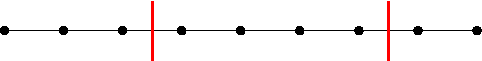
\includegraphics{Images/fig-1DIsingdisorder.pdf}
    \caption{Cartoon of the setup for Landau's argument for disorder in the 1D Ising model. We consider flips in the bonds between spins (domain walls) in the chain of spins.}
    \label{fig-1DIsingdisorder}
\end{figure}

The Hamiltonian is minimized if all spins are aligned. The next lowest energy state is one where there is a single flipped spin. Compared to the lowest energy state, this has energy penalty $-2J$ and so has a boltzmann factor $e^{-2J/k_B T}$ that suppresses the probability of this happening. So up to an overall factor $e^{JN/k_B T}$ which takes into account the zero point energy, the first twoo terms in the partition function (the low-$T$ expansion) is:
\begin{equation}
    Z \sim 1 + Ne^{-2J/k_B T}
\end{equation}
with the $N$ appearing as these are the possible bonds (domain walls) between spins that could be flipped. Then we add the next term for 2 flips, which yields:
\begin{equation}
    Z \sim 1+ Ne^{-2J/k_B T} + \binom{N}{2}e^{-4J/k_B T}
\end{equation}
and in general the term with $n$ flipped bonds has coefficient $\binom{N}{n}$ and so:
\begin{equation}
    Z \sim 1 + Ne^{-2J/k_B T} + \binom{N}{2}e^{-4J/k_B T} + \ldots + \binom{N}{n}e^{-2nJ/k_B T} + \ldots
\end{equation}
now, if we look at the most likely distribution, we see that the $n = N/2$ unmagnetized state is favoured. The entropy grows faster than the number of bonds, vs. the energy grows proportionally than the number of bonds; so the entropy wins out and we see that the unmagnetized state is favoured.

Why does this argument fail in higher dimensions? Because the domain walls scale differently in 2D. The entropy grows as the number of closed paths (rather than as the number of points on the line) which means that the above argument does not apply in the same way (and we do get a phase transition in higher dimensions)!

Lots of cool stuff that Ising models can be tied to... e.g. Majorana fermions in 2D, random surface theories, fermionic string theories in 3D...

\subsection{Teaser - Infinite Range Ising Model}
We look at another analytically solvable Ising model. Here, we remove the restriction that the spins only interact with their nearest neighbours. Specifically, we consider the case where every spin interacts with every other spin with the same interaction strength. While this is not at all a physically realistic system (because interactions are not infinite range in real life, of course) but we will see that the phase diagram of this model is more interesting, with phase transitions occuring at finite $T$ across $B = 0$. 

Our Hamiltonian is:
\begin{equation}
    H = -\frac{J}{N}\sum_{n, n'}\sigma_n \sigma_{n'} - B\sum_n \sigma_n
\end{equation}
where the sum $\sum_{n, n'}$ runs over all pairs of spins in the lattice. We are able to evaluate this by summing over one spin at a time (with each spin giving an equal contribution to the overall partition function), because all spins look the same here:
\begin{equation}
    Z = \sum_{\sigma_n} e^{\frac{J}{k_B T}\sum_{n, n'}\sigma_n \sigma_{n'} + \frac{B}{k_B T}\sum_n \sigma_n}
\end{equation}
This looks awful, but we can consider an analogy with a Gaussian integral. Consider:
\begin{equation}
    \int_{-\infty}^\infty dm e^{-\left(m - \frac{1}{N}\sum_x \sigma_x\right)^2\frac{JN}{k_B T}}
\end{equation}
We can solve this by translating the integral to get rid of $\sum_x \sigma_x$ which is a constant w.r.t. the variable of integration. The integral then evaluates to:
\begin{equation}
    \int_{-\infty}^\infty dm e^{-\left(m - \frac{1}{N}\sum_x \sigma_x\right)^2\frac{JN}{k_B T}} = \sqrt{\frac{k_B T}{NJ}\pi}
\end{equation}
So then:
\begin{equation}
    1 = \sqrt{\frac{NJ}{\pi k_B T}}\int_{-\infty}^\infty dm e^{-\left(m - \frac{1}{N}\sum_x \sigma_x\right)^2\frac{JN}{k_B T}}
\end{equation}
Now let us put this factor of 1 into the partition function. We will then see that terms cancel, and we get an integral that we can solve - if $N$ is large - using a saddle point integration technique. From this we can obtain the free energy and learn the thermodynamic properties of the system.
\newpage
\section{The Infinite Range Ising Model}
\subsection{Motivation - Mean Field Theory}
The Hamiltonian of the infinite range Ising model is:
\begin{equation}
    H = - \frac{J}{N}\sum_{x, y}\sigma_x \sigma_y - B\sum_x \sigma_x
\end{equation}
The sum is taken over all pairs of spin, so every spin interacts with the same interaction strength as every other spin. This is obviously unrealistic physically, but it is of interest to study as the solution gives us insight into mean field theory, which is a approximation technique that can tell us a lot about second-order phase transitions.

Why is this? We can move the sum $\frac{1}{N}\sum_y$ inside of the $\sum_x$ summation, and then this looks like the spin $\sigma_x$ interacts with the mean/average spin $\frac{1}{N}\sum_y \sigma_y$ (this is analytically true for this model). Note that mean field theory is wrong in general (it is an approximation technique) but it is a widely used tool (e.g. in condensed matter theory).

\subsection{Gaussian Integral}
Recall from our teaser last time the identity:
\begin{equation}
    1 = \left(\frac{NJ}{\pi k_B T}\right)^{1/2}\int_{-\infty}^\infty d\phi e^{-\frac{NJ}{k_B T}\phi^2}
\end{equation}
How is this integral evaluated? This is a classic integral; let's go through it together. Let's consider the general (1-D) Gaussian integral:
\begin{equation}
    \int_{-\infty}^\infty dx e^{-ax^2}
\end{equation}
The trick is to write the above as a square root of its square:
\begin{equation}
    \int_{-\infty}^\infty dx e^{-ax^2} = \sqrt{\left( \int_{-\infty}^\infty dx e^{-ax^2}\right)^2} = \sqrt{\left( \int_{-\infty}^\infty dx e^{-ax^2}\right)\left(\int_{-\infty}^\infty dy e^{-ay^2}\right)}
\end{equation}
Now this looks like a 2-dimensional integral; one we can solve by going into polar coordinates!
\begin{equation}
    \int_{-\infty}^\infty dx e^{-ax^2} = \sqrt{\int_{-\infty}^\infty dxdy e^{-a(x^2 + y^2)}} = \sqrt{\int_{0}^{2\pi}d\phi \int_{0}^\infty rdr e^{-ar^2}}
\end{equation}
Now making the substitution $u = ar^2$, $du = 2ardr$, the integral is easily solved:
\begin{equation}
    \int_{-\infty}^\infty dx e^{-ax^2} = \sqrt{2\pi \frac{1}{2}\frac{1}{a}} = \sqrt{\frac{\pi}{a}}
\end{equation}
which is the familiar result.

\subsection{Solving the Infinite Range Ising Model}
Now, let us take this result, and consider that we can shift the variable of integration $\phi \to \phi + \sum_x \sigma_x$ (plus a constant - does not change the result of the integral as the range of integration is $-\infty$ to $\infty$):
\begin{equation}\label{eq-1convenientform}
    1 = \left(\frac{NJ}{\pi k_B T}\right)^{1/2}\int_{-\infty}^\infty d\phi e^{-\frac{NJ}{k_B T}\left(\phi - \frac{1}{N}\sum_x \sigma_x\right)^2}
\end{equation}
Now, recall back to the partition function for the model we wish to compute:
\begin{equation}
    Z[T, B, N] = \sum_{\text{spins}} e^{\frac{J}{Nk_B T}\sum{x, y}\sigma_x\sigma_y + \frac{B}{k_B T}\sum_x \sigma_x}
\end{equation}
Now let us insert a factor of $1$ as in Eq. \eqref{eq-1convenientform}; this will yield some useful cancellations:
\begin{equation}
    Z[T, B, N] = \left(\frac{NJ}{\pi k_B T}\right)^{1/2}\int_{-\infty}^\infty d\phi e^{-\frac{NJ}{k_B T}\phi^2}\sum_{\text{spins}} e^{\frac{B + 2J\phi}{k_B T}\sum_x\sigma_x}
\end{equation}
Now, the sum over spins can be carried out explicitly as we can just independently sum over and take the product:
\begin{equation}
    \sum_{\text{spins}} e^{\frac{B + 2J\phi}{k_B T}\sum_x\sigma_x} = \left(e^{\frac{B + 2J\phi}{k_B T}} + e^{-\frac{B + 2J\phi}{k_B T}}\right)^N
\end{equation}
Recognizing the identity $e^{x} + e^{-x} = 2\cosh(x)$, our partition function becomes:
\begin{equation}
    Z[T, B, N] = \left(\frac{NJ}{\pi k_B T}\right)^{1/2} \int_{-\infty}^\infty d\phi e^{-N\left[\frac{J}{k_B T}\phi^2 - \ln(2\cosh(\frac{B + 2J\phi}{k_B T}))\right]}
\end{equation}
So we are left with an integral that is hard. What do we do? Remember that we are doing stat mech/thermo here, so $N \to \infty$. In this case, we can evaluate this integral by the saddle point technique. We replace the integral with where the integrand is maximized\footnote{Note: we are allowed to search in the complex plane; more formally, we have an integral over the real line, the contour which we then deform off the real axis such that the contour follows the ``mountain passes'' in the complex landscape. Here this is not so complicated, as we have real solutions.}:
\begin{equation}
    Z[T, B, N] \approx e^{-N\inf_\phi\left[\frac{J}{k_B T}\phi^2 - \ln(\cosh(\frac{B + 2J\phi}{k_B T}))\right] + N\ln 2}
\end{equation}
where $\inf$ (infimum) denotes the greatest lower bound. So then the Helmholtz free energy is:
\begin{equation}
    F[T, B, N] = k_B T N \inf_\phi \left(\frac{J\phi^2}{k_B T} - \ln\cosh\frac{B + 2J\phi}{k_B T}\right) - k_B T N\ln 2
\end{equation}
So, we should try to find this infimum/minimum; of course this is a calculus problem, which we can solve by taking the derivative and setting the expression to zero:
\begin{equation}
    \frac{2J}{k_B T}\phi - \frac{2J}{k_B T}\tanh \frac{B + 2J\phi}{k_B T} = 0
\end{equation}
We then look for solutions to the expression:
\begin{equation}\label{eq-phitranscendental}
    \phi = \tanh \frac{B + 2J\phi}{k_B T}
\end{equation}
which when graphically plotted, appears as in Fig. \ref{fig-phitranscendental}.

\begin{figure}[htbp]
    \centering
    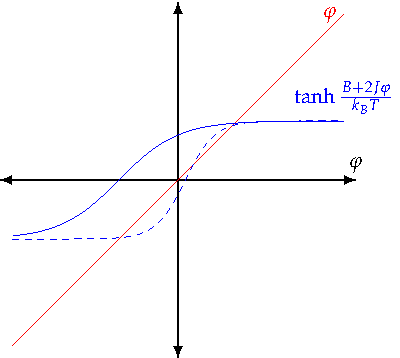
\includegraphics{Images/fig-phitranscendental.pdf}
    
    \caption{Plot of the LHS (red) and RHS (blue - solid line with $\frac{B}{k_BT} = \frac{2J}{k_BT} = 1$) of Eq. \eqref{eq-phitranscendental} as a function of $\phi$. There always exists one solution to the transcendental equation, and depending on $B$, there may exist 3 solutions (blue - dashed line with $\frac{B}{k_BT} = -\frac{1}{4}, \frac{2J}{k_BT} = 2$).}
    \label{fig-phitranscendental}
\end{figure}

It should be clear from the graph and the behavior of $\tanh$ at $\pm \infty$ (going to $\pm 1$) that we are guaranteed to have at least one solution to this expression (note that for a smaller range of $B$s, it is also possible to have three solutions). If we only have one solution, it is easy to determine which is the minimum. If we have three, we have to decide between the three; but the minimum will still be the furthest to the right (except in the case when $B = 0$, in which case the leftmost and rightmost solutions are degenerate).

Note that if we take the second derivative and plug in our solution at the minimum, we get the curvature at the minimum:
\begin{equation}
    \frac{2J}{k_B T} - \left(\frac{2J}{k_B T}\right)^2 + \left(\frac{2J}{k_B T}\right)^2\tanh^2\frac{B + 2J\phi}{k_B T}
\end{equation}
So, if the temperature is large enough, that is, $\frac{2J}{k_B T} - \left(\frac{2J}{k_B T}\right)^2$ is always positive, since the $\tanh^2$ term is always positive the second derivative of the function is always positive. So, the function is convex, and there exists one unique minimum. Specifically, this occurs when 
\begin{equation}
    T > \frac{2J}{k_B} = T_c.
\end{equation}
Conversely, when $T < T_c$ the first term can fluctuate between being positive and negative and we get two minima (Mexican hat).

\begin{figure}[htbp]
    \centering
    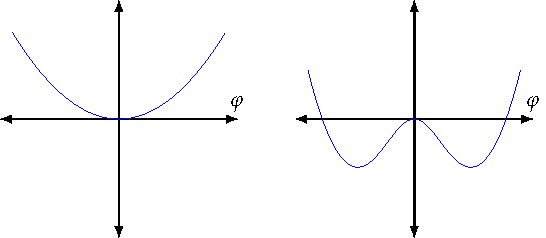
\includegraphics{Images/fig-infIsingphasetrans.pdf}


    \caption{Plot of $\frac{J\phi^2}{k_B T} - \ln\cosh\frac{B + 2J\phi}{k_B T}$ in the cases where $T > T_c$ (left - with $B = 0$ and $\frac{J}{k_B T} = \frac{1}{5}$) and $T < T_c$ (right - with $B = 0$ and $\frac{J}{k_BT} = 1$). I made a desmos graph \href{https://www.desmos.com/calculator/5d74tk33yd}{here} where you can play with $J, B$ and see how this changes the function.}
    \label{fig-infIsingphasetrans}
\end{figure}

This tells us that something ``happens'' at $T = T_c$ (specifically, a phase transition)! Note if we set $B = 0$, then the Hamiltonian has higher symmetry $\ZZ_2$; the Hamiltonian is unchanged under spin flips. So in this case the magnetization goes to zero (which we will see shortly can be identified with $\phi$). And we can also show mathematically that if $B = 0$ then the magnetization goes to zero. But if $B \neq 0$ we can have $T < T_c$, in which case $\phi = 0$ is actually a local maximum. So if $T < T_c$ we see ferromagnetism; spontaneous magnetization occurs due to the turning on of a magnetic field and a decrease in temperature.

Sketching the phase diagram for the infinite range Ising model, we have a significant difference to the standard $D = 1$ Ising model; the first phase transition persists at finite temperature at $B = 0$ (where we have the crossover of magnetization, as we go from one minimum of finite magnetization to the other (with opposite sign)). At $T = T_c$, the two minima solutions merge; they don't dissapear (really), but they go off into the complex plane where we don't have to worry about them anymore, and the $B = 0$ maxima becomes the minimum. We will see in a few moments that this is a second order phase transition!

\begin{figure}[htbp]
    \centering
    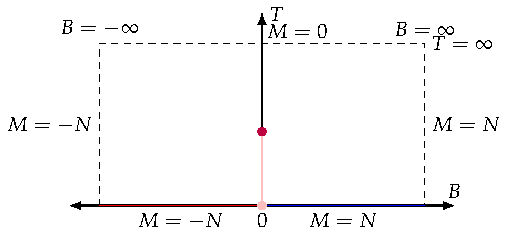
\includegraphics{Images/fig-IsingphasediagramB0.pdf}
    
    \caption{Sketch of the phase diagram of the infinite range Ising model. The first order phase transition at $B = 0$ persists at finite temperature, and at the critical temperature $T = T_c$ we have a second order phase transition.}
    \label{fig-infIsingphasediagram}
\end{figure}

For a second order phase transition, the free energy is smoother at the transition point; the first derivative exists.

\subsection{Analysis Near the Critical Temperature}
Can we be a little more analytic here? It's not so simple as we have these awful functions we are trying to minimize. If $\frac{B}{k_B T}$ is ``small'' and $T \sim T_c$ then $\phi$ is also small. Then, we are able to approximate these formulas by Taylor expanding in $\phi$ and $B$. An approximate form of the free energy reads:
\begin{equation}
    F[T, B, N] = Nk_B T \inf_\phi \left[\frac{J\phi^2}{k_B T} - \frac{1}{2}\left(\frac{2J\phi}{k_B T}\right)^2 + \frac{1}{12}\left(\frac{2J\phi + B}{k_B T}\right)^4 + \ldots \right] - k_B T N \ln 2 
\end{equation}
where we have used $\ln\cosh x = \frac{x^2}{2} + \frac{x^4}{12} + O(x^6)$. Let's analyze this expression when $B = 0$:
\begin{equation}
    F[T, B = 0, N] = -N\inf_\phi \left[J\left(1 - \frac{T_c}{T}\right)\phi^2 + \frac{1}{12}\left(\frac{T_c}{T}\right)^4\phi^4 + \ldots \right]
\end{equation}
where we have absorbed $\frac{1}{k_B T}$ into the expression inside of the infinum and used that $T_c = \frac{2J}{k_B}$.
When $T > T_c$, the solution is easily read off as $\phi = 0$. When $T < T_c$, things are a bit trickier; taking a derivative by $\phi^2$ and setting things to zero we get:
\begin{equation}
    \frac{J}{k_B T}\left(1 - \frac{T_c}{T}\right) + \frac{1}{6}\left(\frac{T_c}{T}\right)^4 \phi^2 = 0
\end{equation}
so then:
\begin{equation}
    \phi = \pm \sqrt{K\left(-1 + \frac{T_c}{T}\right)}
\end{equation}
where $K$ is some number. The free energy is then:
\begin{equation}
    F = \begin{cases}
        C & T > T_c
        \\ C + K\left(\frac{T_c}{T} - 1\right)^2 & T < T_c
    \end{cases}
\end{equation}
What we are really interested in here is how many derivatives we can take here before things go awry. It is clearly 2; when we take the first derivative, things are still continuous at $T_c$ where $F' = 0$. Taking two derivatives, we find that this is no longer continuous where at $T_c$ there is a jump from $F'' = 0$ to $F''$ some positive nonzero constant.

\subsection{Magnetization and Critical Exponents}
Now, let's try to interpret $\phi$ physically. It turns out to be the magnetization. One can argue this from the initial expression, or by calculating the magnetization explicitly:
\begin{equation}
    M = \left.-\dpd{F}{B}\right|_{T, N} = N\tanh \frac{2J\phi + B}{k_B T} = N\phi
\end{equation}
where we have used Eq. \eqref{eq-phitranscendental} in the last equality. From this we conclude:
\begin{equation}
    m = \frac{M}{N} = \phi.
\end{equation}
So all of our analysis of $\phi$ was indeed an analysis of a physical quantity. 

Another thing we can do is to set $T_c$ and approach the phase transition by varying $B$. We note that:
\begin{equation}
    m(T = T_c) \sim B^{1/3}
\end{equation}
\begin{equation}
    m(B = 0) \sim (T_c - T)^{1/2} \quad T < T_c
\end{equation}
\begin{equation}
    F \sim (T_c - T)^2 \quad T < T_c
\end{equation}
what we are interested in is the scaling behavior of $T$; these are known as critical exponents. Specifically here we are finding the critical exponents of mean field theory. This is quite profound; if a transition is described by mean field theory, they have the same critical exponents. Phase transitions with the same critical exponents have the same universality class. This was realized by Landau, who formalized the Landau theory of phase transitions. There is not much missing here from the Landau theory; the only thing which was missing is the correlation length of the system (which makes no sense for the infinite range Ising model, anyway). Note that (for systems where it is meaningful to discuss correlation lengths) the correlation lengths diverge at the phase transition, and the way these diverge are of interest indeed.

Note that it was unclear as to whether Landau theory was correct or wrong for a while; however when the 2D Ising model was solved, it was found to not have the same critical exponents as the Landau prediction (note that this does not mean that Landau theory is incorrect, only that 2D Ising lies in a different universality class. Note that for $D > 4$, Ising models are in fact well described by Landau theory/mean field theory).

Let us consider some parameters/quantities that are of interest to study when we consider phase transitions. We call $\boxed{m}$ the \emph{order parameter} in the Landau framework; the expectation value of the magnetization (per spin) tells us about the symmetry of the system (and, here, the fact that the $\ZZ_2$ symmetry is spontaneously broken at $B = 0$). We also have the (normalized) distance $\boxed{\tau}$ from the critical temperature:
\begin{equation}
    \tau = \frac{T - T_c}{T_c}
\end{equation}
We have the magnetic field $\boxed{B}$. We have the susceptibility $\boxed{\chi}$ which is:
\begin{equation}
    \chi \sim \dpd{m}{B}
\end{equation}
i.e. if we vary the field, how does the magnetization change. At the critical point, this tends to diverge. We also have the correlation length $\boxed{\xi}$ which is given by:
\begin{equation}
    \avg{\sigma_x \sigma_y} \sim e^{-\frac{1}{\xi}\abs{x - y}}
\end{equation}
where $\boxed{\avg{\sigma_x \sigma_y}}$ is a correlation function. If we drop down from the infinite range model to the standard Ising model, another parameter to consider is the dimension of the model $\boxed{D}$. We also have the specific heat $\boxed{C}$:
\begin{equation}
    C \sim \frac{T}{N}\dpd{^2F}{T^2}
\end{equation} 
We also have critical exponents (a whole family of them...). For above the phase transition $\tau > 0$, we have:
\begin{equation}
    C \sim \tau^{-\alpha}
\end{equation}
\begin{equation}
    \tau \sim \tau^{-\gamma}
\end{equation}
\begin{equation}
    \xi \sim \tau^{-\nu}
\end{equation}
below the phase transition $\tau < 0$ we have the same idea, but we put a prime on things to distinguish:
\begin{equation}
    C \sim \tau^{-\alpha'}
\end{equation}
\begin{equation}
    \tau \sim \tau^{-\gamma'}
\end{equation}
\begin{equation}
    \xi \sim \tau^{-\nu'}
\end{equation}
We also have that the order parameter scaling as:
\begin{equation}
    m \sim \tau^{\beta}
\end{equation}
for $\tau = 0, B = 0$, we have:
\begin{equation}
    B \sim m^\delta
\end{equation}
\begin{equation}
    \avg{\sigma_x\sigma_y} \sim \frac{1}{\abs{x - y}^{-d + 2 - \eta}}
\end{equation}

What we have found through our analysis is a bunch of these critical exponents. Mean field theory makes the following predictions:
\begin{equation}
    \alpha = \alpha' = 0
\end{equation}
\begin{equation}
    \beta = \frac{1}{2}
\end{equation}
\begin{equation}
    \gamma = \nu' = 1
\end{equation}
\begin{equation}
    \delta = 3
\end{equation}
We don't learn things about the correlation lengths from this model as the interactions are infinite range; but this can be fixed up via Landau-Ginsberg theory, which tells us:
\begin{equation}
    \eta = 0
\end{equation}
\begin{equation}
    \nu = \frac{1}{2}
\end{equation}
Experimental values for comparison can be compared with the table posted on the course webpage. These are not that easy to measure because they involve the scaling of something at a critical point. But some can be measured; for example $\alpha$ for the $\lambda$-transition (Bose condensation transition) in liquid Helium-4 is experimentally determined to be:
\begin{equation}
    \alpha = -0.0127 \pm 0.0003
\end{equation}
so it is known to be nonzero. So mean field theory does not quite describe this transition, though it comes close. In the theory, $\alpha = 0$ as $F \sim T^2$ and hence specific heat is a constant.
\newpage
\section{Landau Theory}

% Example oral exam q: Difference between canonical and microcanonical ensemble
% Example oral exam q: What is Landau theory

\subsection{Introduction and Motivation}
Last time, we discussed the infinite-range Ising model. It is a nice model that we can write down and solve analytically. We ended last lecture by calculating the critical exponents of the model. This model does have some shortcomings; of course it is completely physically unrealistic, and it also does not let us calculate correlation functions (and there are some critical exponents that come from these). A lot of the discussion of it was poached from Pairisi's book on statistical field theory; there he has a hand-wavey argument about how to get correlation functions from the model (which Gordon does not understand - so we do something else)! 

We note that if we are interested in the behaviour near the singular points (i.e. characterizing the critical exponents) then a lot of the fine-grained details of the model does not matter. We introduced Landau theory, which predicts the same (mean-field) critical exponents as the infinite range Ising model, but also can do more - e.g. providing us with the correlation function for spins. The main attribute which we discussed and which we will continue to discuss is the correlation length, which describes the (exponential) degree to which correlations die off with distance\footnote{We will have the machinery to explain why this decay is exponential by the end of the course. For now, we take it as a result.} The correlation length has a power law behaviour, and the exponent on the $\frac{1}{\abs{x - y}}$ also is a critical exponent.

\subsection{The Landau Potential and Free Energy}
To discuss correlation functions, we require some position-dependent behavior. A motivation for how to do this - iron has some microscopic (fine-grained) crystal structure, but macroscopically the iron looks like a continuum and we cannot see the lattice. In this limit, we see the magnetization smoothly varying like a continuous field. So, let us write down the Landau potential:
\begin{equation}
    \Gamma[\phi] = \int dx \left[\tau \frac{\phi^2(x)}{2}  + \lambda \frac{\phi^4(x)}{4!} -B(x)\phi(x) + \frac{1}{2}\nabla \phi \cdot \nabla \phi\right]
\end{equation}
where $\tau \sim \left(\frac{T}{T_c} - 1\right)$, $\lambda$ is some (positive) coupling constant, and $B$ is the magnetic field strength. The first three terms already looks like a Hamiltonian, but we want something to ``smooth it out'' as with just those three each point is independent of one another and there is nothing stopping some very large fluctuations in $\phi$. So the last term penalizes this, by ensuring that large fluctuations are unfavourable. Note that Landau theory is also able to acommodate different kinds of spins, e.g. not just $\pm 1$ at each site but pointing in some arbitrary direction (but for now let us just stick with the simplest case).

Now, the idea is to get the free energy as:
\begin{equation}
    F = \inf_\phi \Gamma[\phi]
\end{equation}
and this gets us into the realm of variational calculus/functional calculus. This is because $\Gamma$ is a functional - it is a function of the field $\phi$ which itself is a function of position. We wish to minimize $\Gamma$ over all $\phi$s, which requires some functional calculus in general; but here this is not necessary.

If $B \leq 0$ and $\tau > 0$, then all the terms are positive and so the easy minimum is taking $\phi = 0$. 

If $B = 0$ and $\tau < 0$, then now things are not so trivial. In this case we write the potential as:
\begin{equation}
    \Gamma = \int dx \left[\frac{1}{2}\nabla \phi \cdot \nabla \phi + \frac{\lambda}{4!}\left(\phi^2 + \frac{\tau 4!}{4\lambda}\right)^2 - \frac{\lambda}{4}\left(\frac{\tau 4!}{4\lambda}\right)^2\right]
\end{equation}
Here, the potential is minimized if the first two terms vanish (the last term is just a constant). The first term is minimized if $\phi$ is a constant, and the second (positive) term is then minimized by taking it to zero:
\begin{equation}
    \phi = \pm \sqrt{\frac{4!}{4\lambda}(-\tau)}
\end{equation}
and here we already recover the square root scaling of the magnetization (i.e. the critical exponent of $\frac{1}{2}$) that we discussed last class.

Now, let us plug the minimizing $\phi$ back into $\Gamma$ and solve for the free energy $F$:
\begin{equation}
    F = \begin{cases}
        0 & B \leq 0, \tau > 0
        \\ V\frac{\lambda}{4}\left(\frac{4!}{4\lambda}\right)^2\tau^2 & B = 0, \tau < 0
    \end{cases}
\end{equation}

\subsection{Finding Critical Exponents; Specific Heat, Equation for $\phi$, Susceptibility}
Now, the specific heat can be obtained as:
\begin{equation}
    C = -T\dpd{^2F}{T^2} \sim \begin{cases}
        \abs{\tau}^{-\alpha} & \tau > 0
       \\  \abs{\tau}^{-\alpha'} & \tau < 0
    \end{cases} \quad \alpha = \alpha' = 0
\end{equation}
where the critical exponents are found to be zero because there is no singularity! Again we recover the mean-field critical exponents from alst time.

The next critical exponents are not quite as simple to calculate, but they also aren't that bad. We consider the equation for $\phi$; this can be obtained by doing a variational minimization of $\Gamma$:
\begin{equation}
    (-\nabla^2 + \tau)\phi + \frac{\lambda}{3!}\phi^3 - B = 0
\end{equation}
If we assume $\phi$ is a constant and $\tau = 0$ (i.e. $T = T_c$) then we find:
\begin{equation}
    \phi \sim B^{1/3}
\end{equation}
or equivalently:
\begin{equation}
    B \sim \phi^3
\end{equation}
which is another critical exponent (that we recover last time). Every exponent we derive here will agree with what we found last class, and we can further define more.

Recall the susceptibility, defined as:
\begin{equation}
    \chi = \dpd{m}{B}
\end{equation}
Note that while $\phi$ is more general than $m$, after we have solved everything, we can identify $m = \phi$. To this end, we should explore how this solution $\phi$ changes as we vary $B$. Again assuming that $\phi$ does not vary in position, we have:
\begin{equation}
    \tau \phi + \frac{\lambda}{3!}\phi^3 - B = 0
\end{equation}
Taking the derivative w.r.t. $B$ we find:
\begin{equation}
    \left(\tau + \frac{\lambda}{2!}\phi^2\right)\dpd{\phi}{B} - 1 = 0
\end{equation}
We then find that:
\begin{equation}
    \chi \sim \begin{cases}
        \frac{1}{\tau} & \tau > 0
        \\ -\frac{1}{2\tau} & \tau < 0
    \end{cases}
\end{equation}
this is called the \emph{Curie-Weiss Law} (and also gives us two more critical exponents). This is not an exact fit to the experimentally measured susceptibility of Iron, but it was close enough that it did take a little while to notice a discreptancy.

\subsection{Calculating Correlation Functions}
To actually calculate a correlation function, we need to re-introduce spatial dependence into our field. We are interested in the eqaution:
\begin{equation}
    \left(-\nabla^2 + \tau + \frac{\lambda}{2!}\phi^2(x)\right)\chi(x, y) = \delta(\v{x} - \v{y})
\end{equation}
where:
\begin{equation}
    \chi(x, y) = \avg{m(x)m(y)} - \avg{m(x)}\avg{m(y)}
\end{equation}
is the connected correlation function. Note that our problem has now reduced to finding a Green function. The standard way to approach this is a plane wave ansatz/fourier transform.

Let us study the special case of $\tau = 0$ ($T = T_c$) and $\phi = 0$. In this case, we have the very simple equation:
\begin{equation}
    -\nabla^2 \chi = \delta(\v{x} - \v{y})
\end{equation}
if $D = 3$, then this is just the famous Coloumb potential and so the solution is:
\begin{equation}
    \chi = \frac{1}{4\pi \abs{\v{x} - \v{y}}}
\end{equation}
where here the critical exponent is $\eta = 0$ (recalling that $\chi \sim \frac{1}{\abs{\v{x} - \v{y}^{-D + 2 - \eta}}}$). 

A question to test your mathematical intuition - what do solutions to this equation look like in other dimensions? By dimensional analysis, we have:
\begin{equation}
    \chi \sim \frac{1}{\abs{\v{x} - \v{y}}^{D - 2}}
\end{equation}
and so $\eta = 0$ in any dimension for this special case, actually! A quick review of the dimensional analysis argument; $[\delta] = [X]^{-d}$ (i.e. inverse of the dimension) and so I want something which taking two spatial derivatives (i.e. subtract two dimensions) yields dimensions of $-D$ and so the dimensions of $\chi$ must be $-D + 2$. 

Away from the critical point when $\tau \neq 0$, things look bad; but then it is balanced out by $\frac{\lambda}{2!}\phi^2(x)$... then we have to be a bit more sophisticated, and consider that the Green function decays exponentially, i.e. know that $\chi(x, y) \sim e^{-\abs{x-y}/\eta}$. The coefficient can be obtained via dimensional analysis, again; the argument of a transcendental function must be dimensionless, and so we conslude that:
\begin{equation}
    \eta = \frac{1}{\tau^{1/2}}
\end{equation}
The last thing we have not derived is how this exponential decay comes about. We could do this by taking the fourier transform of the equation, then for large $\abs{\v{x} - \v{y}}$ carry out the integral via saddle point technique which gives the exponential decay.

\subsection{Parameters in Landau Theory}
What are parameters/inputs into the Landau theory? Note that since the integral goes over the volume, the number of spins is implicitly included. So we won't bother even including this on our list. 
\begin{enumerate}[(i)]
    \item $\tau \sim (T - T_c)$.
    \item Dimension $D$ - it appears in the integral, and in the derivatives, and if we have to solve the differential equation, this of course would highly depend on the dimensionality of the model.
    \item Symmetry and number of components of magnetization (here just one - $\phi$ is a function spits out one real number). Also, the fact that $\Gamma$ has a zero is encoded by the fact that the theory is symmetric under interchange of $\phi \leftrightarrow -\phi$ (if one also puts $B \leftrightarrow -B$).
    \item $\lambda > 0$ - Required for stability of the model.
\end{enumerate}
This is not very many parameters, but we get a lot of output out of it!

When this is applied to a superconductor, then this becomes Landau-Ginzberg theory (one puts in the electromagnetic field in the natural way).

One more comment about Landau theory - it can be used to describe first order phase transitions, in addition to second order phase transitions. We can add more terms, then we get two (or more) extrema with an energy barrier between them. The first order phase transition (e.g. bubble nucleation) will be when the two extrema have the same energy (the crossover point when they are both the global minima). There is less to study here as there are no associated critical exponents, but it is nevertheless something that the theory is capable of accommodating. 

Q - as it is, this looks identical to the massless scalar field theory with $m = \tau$ if $B = 0$. Is there a deeper correspondence? The answer will turn out to be yes, as we will learn as the term progresses (there is identical mathematical structure here, but it is worth noting that the theory here is completely classical). Somehow Landau guessed the classical limit of quantum field theory from this modelling.

\subsection{$O(3)$ (Vector) Model}
If we want to analyze something else, e.g. a piece of iron where the magnetization can point in some arbitrary direction in $\RR^3$, we can modify the theory we wrote above by changing $\phi$ to be a three-component function $\gv{\phi}$ (and $B \to \v{B}$ to be a three-component field, rather than just a projection along a single axis). 

This is called the $O(3)$ model as the spins can point in three directions. Note that we can still place our lattice in an arbitrary dimension. We could also allow our spins to point in more directions ($O(N)$ model). Our field is now a vector:
\begin{equation}
    \gv{\phi} = \m{\phi_1 \\ \phi_2 \\ \phi_3}
\end{equation}
Our Landau potential genrealizes in the expected way:
\begin{equation}
    \Gamma = \int d^3x \left(\frac{1}{2}\nabla_i \phi_j\nabla_i \phi_j + \frac{\tau}{2}\gv{\phi}^2 + \frac{\lambda}{4!}\left(\gv{\phi}^2\right)^2 - \v{B} \cdot \gv{\phi}\right)
\end{equation}
Note that we are allowed to add another term, actually; in three dimensions there is a further rotational symmetry (we can rotate the space and leave the space the same, or now we can rotate the spins and leave the space the same). So, we could add a term of the form $(\nabla \cdot \gv{\phi})^2$ - but this would have less symmetry (e.g. we could add this term in the case where we have phonons in the lattice, which breaks this two-fold rotational symmetry; we would have to rotate the space and the lattice. This added term corresponds to this broken two-fold rotational symmetry, as the function is no longer invariant under the two types of rotations).

To go to superconductivity, there is a breakdown of phase symmetry of the wavefunction, so we add a complex phase function (and then this becomes Landau-Ginzeberg theory, but we don't discuss this here).

\subsection{Teaser - Spherical Model}
Next class we will discuss how Landau theory is actually wrong. One demonstration of this was the exact solution of the 2D Ising model, which does not agree with the mean field Landau theory predictions. 

The spherical model will provide us another route to showing how Landau theory is not correct. It is in some sense a simplified Ising model, and one which we will be able to solve analytically (somewhat).

The Hamiltonian is given by:
\begin{equation}
    H = -J\sum_{x, i}\sigma_x \sigma_{x + i} - B \sum_x \sigma_X
\end{equation}
where the spins sit on a regular lattice in an arbitrary dimension (a line in 1D, a square lattice in 2D, a cubic lattice in 3D, a hypercube in 4D and so on...) $i$ labels the connections between the lattice sites, and there is a coupling of neighbours (e.g. see Fig. \ref{fig-2DIsing}).

This looks like the Ising model (and has the same Hamiltonian) but it is not the Ising model. This is because we will allow $\sigma_x$ to be any real number, not just $\pm 1$, rather $\sigma_x \in (-\infty, \infty)$. This simplifies things because continuous math is easier than discrete math.

The obvious problem with this is it seems as though we can have an arbitrary amount of magnetization to the system (and hence the model is unstable); we therefore impose the constraint:
\begin{equation}
    \sum_x \sigma_x^2 = N
\end{equation}
where $N$ is the number of sites. While it is not obvious, one is able to show that all spins pointing up or downwards is the degenerate energy minima of the system.

Next time, we will be able to ``solve'' the system (up to some leftover functions) and we will be able to analyze the critical exponents of the model. For dimensions $D \geq 4$ we will find that the critical exponents match exactly those of Landau/mean field theory. For $D < 4$ this is not the case. 
\newpage
\section{The Spherical Ising Model}

\subsection{Review and Introducing the Model}
Last time we gave a teaser about the spherical model; note that historically, the exact solution to the 2D Ising model was actually discovered first (though the spherical model is much easier to solve, which is why we discuss it first)! We work out the phase diagram of what is basically a ferromagnet.

\begin{figure}[htbp]
    \centering
    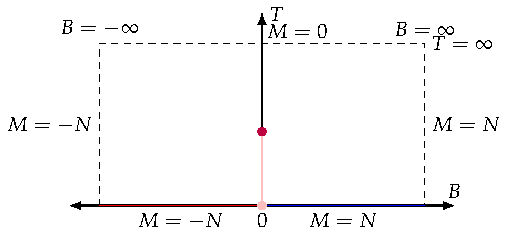
\includegraphics{Images/fig-IsingphasediagramB0.pdf}
    \caption{Phase diagram of infinite range Ising model and Spherical model.}
    \label{fig-sphericalmodelphasediagram}
\end{figure}

In 1D, we found spontaneous symmetry breaking at $B = 0, T = 0$. In the infinite range model, we found that this behaviour persists at finite temperature (with a first-order phase transition line) and culminating in a second-order phase transition point at $B = 0, T = T_c$. We studied the behaviour of the phase diagram in the vicinity of $T_c$. We observed the phenomena of universality, which in a practical sense told us that all that matters to determine the critical phenomena were the first few terms of the Taylor expansion of the free energy, and any model that produced the same coefficients have the same critical exponents - those of mean field theory. Presumably, if we found something else that was not mean field theory, it would still not depend on very much. Gordon isn't aware of a rigorous way of showing that a certain system is in a particular universality class, but even with this missing, it is thrown around in research seminars as if we understand this fully; so it is good to understand the terminology.

The spherical model is another model, and it will have the same phase diagram as the infinite range Ising model; the new thing will be that some of the critical exponents are \emph{not} mean field, which will tell us that mean field theory is not everything! Landau conjectured that mean field theory was everything, but by example we can show him to be wrong.

In the Ising model, the spins were discrete $\sigma_x = \pm 1$. In the spherical model, we lift this restriction and allow $\sigma_x \in \RR$. However there is a problem; looking at the exchange term in the Hamiltonian:
\begin{equation}
    H = -J\sum_{x, i}\sigma_x \sigma_{x + i}
\end{equation}
we see that there is no lower bound on the energy (by taking $\sigma_x \to \infty$). In order to ensure that this pathological behaviour does not occur, we introduce the constraint:
\begin{equation}
    \sigma_x \sigma_x^2 = N
\end{equation}
which tells us that on average, $\sigma_x \sim 1$. This bounds the energy from below. We also have the magnetic term, so the full Hamiltonian is:
\begin{equation}
    H = -J\sum_{x, i}\sigma_{x}\sigma_{x + i} - B \sum_x \sigma_x
\end{equation}
note that to generate correlation functions, it is sometimes useful to make $B$ site-dependent:
\begin{equation}
    H = -J\sum_{x, i}\sigma_{x}\sigma_{x + i} - \sum_x B_x\sigma_x
\end{equation}
this makes the model unsolvable, but can be useful for some analysis (e.g. allows us to take derivatives, and then we can set $B$ to a constant).

\subsection{Ground State of the Spherical Model}
Is the ground state (formally this is not a quantum mechanical system so we should say lowest-energy state, but it's hard to resist calling it this) of this model ordered? Let us include the constraint into the Hamiltonian:
\begin{equation}
    \tilde{H} = -J\sum_{x, i}\sigma_x \sigma_{x + i} - B \sum_x \sigma_x + \lambda \left(\sum_x \sigma_x^2 - N\right)
\end{equation}
The equations for the extrema are:
\begin{equation}
    -J\sum_i \left(\sigma_{x + i} + \sigma_{x - i}\right) - B + 2\lambda \sigma_x = 0
\end{equation}
\begin{equation}
    \sum_x \sigma_x^2 = N
\end{equation}
It can be argued that the ground state should be independent of $x$. To this end, let us rewrite the Hamiltonian as follows:
\begin{equation}
    H = \frac{J}{2}\sum_{x, i}\left(\sigma_{x + i} - \sigma_x\right)^2 - JD\sum_x \sigma_x^2 - B\sum_x \sigma_x + \lambda\left(\sum_x \sigma_x^2 - N\right)
\end{equation}
Now, we want to minimize the above. We have a positive function plus something else; so we want to at least get the positive term $\sum_{x, i}(\sigma_{x + i} - \sigma_x)^2$ to zero. This will not interfere with minimizing the rest because the rest of the terms only depend on a single site (so we just minimize per site). Then, we observe that to minimize $\sum_{x, i}(\sigma_{x + i} - \sigma_x)^2$, the $\sigma_x$s should be site independent. This concludes the argument. Having shown this property, we conclude that $\sigma_x^2 = 1$ (i.e. just the average value) and so we find:
\begin{equation}
    \sigma_x = \text{sign}(B), \quad \lambda = DJ + \frac{\abs{B}}{2}, U[T = 0] = -N\left(2DJ + \abs{B}\right)
\end{equation}
We see that the derivative of the energy is discontinuous at $B = 0$. We also see that the magnetization is completely determined by the sign of $B$ (so we have for $T = 0$ that $m = -1$ for $B < 0$ and $m = 1$ for $B > 0$, as we claimed). 

\subsection{Finite Temperature Spherical Model}
If we turn on $T$, we want to find the partition function:
\begin{equation}
    Z[T, B, N] = \int_{-\infty}^\infty \prod_x d\sigma_x e^{-\frac{J}{k_B T}\sum_{x, i} \sigma_x \sigma_{x  + i} + \frac{B}{k_B T}\sum_x \sigma_x}\delta(\sum_x \sigma_x^2 - N)
\end{equation}
where we have enforced the constraint by introducing a dirac delta function into the measure\footnote{Actually, note quite - we are missing the Jacobian term; but it suffices in our case to know that the Jacobian does not grow as the exponential of something, which it does not in this case, so we can neglect it}. To evaluate this, we could write the Dirac delta function as a Fourier integral:
\begin{equation}
    \delta(\sum_x \sigma_x^2 - N) = \int \frac{d\lambda}{2\pi}e^{i\lambda\left(\sum_x \sigma_x^2 - N\right)}
\end{equation}
then evaluate things via the saddle point technique. Instead of doing this - let us solve a simplified version of the model.

\subsection{Mean Spherical Model}
In this simplified version of the model, we replace the constraint $\sum_x \sigma_x^2 = N$ with the constraint that:
\begin{equation}
    \avg{\sum_x \sigma_x^2} = N
\end{equation}
i.e. the configurational average of the sum of the square of the spins is $N$. This still fixes the problem of the Hamiltonian not having a lower bound on the energy, but turns out to be easier to solve. How do we implement this constraint? What we will do is the following; add a term to the exponent:
\begin{equation}
    Z[T, B, N] = \int_{-\infty}^\infty \prod_x d\sigma_x e^{\frac{J}{k_B T}\sum_x \sigma_x \sigma_{x + i} + \frac{B}{k_B T}\sum_X \sigma_x - \mu \sum_x \sigma_x^2}
\end{equation}
In the spherical model proper this would just be adding the constant $-\mu N$ to the model and would do nothing. Here it will have a nontrivial effect. The constraint is implemented by:
\begin{equation}
    \left.-\dpd{}{\mu}\ln Z\right|_{N, T, B} = N
\end{equation}
So, let us calculate the partition function and enforce the above constraint to solve the mean spherical model.

\subsection{Interlude - Gaussian Integral}
Ok, now to solve this model, we will introduce the Gaussian integral\footnote{So long as we can diagonalize $2 \times 2$ matrices and evaluate Gaussian integrals, you're ready to be a theorist, apparently\ldots}. In the course notes the Gaussian integral result is stated but not shown. Here, let's actually walk through it. Let's rewrite the integral for the partition function as:
\begin{equation}\label{eq-Gaussianintegralstart}
    Z[T, B, N]  = \int_{-\infty}^\infty \prod_x d\sigma_x e^{-\frac{1}{2}\sum_{x, y}\sigma_x \Delta(x, y)\sigma_y + \frac{B}{k_B T}\sum_x \sigma_x}
\end{equation}
where:
\begin{equation}\label{eq-Deltaxyspherical}
    \Delta(x, y) = \frac{J}{k_B T}\sum_i\left[2\delta_{xy} - \delta_{x, y+i} - \delta_{x, y - i}\right] + 2\left(\mu - \frac{JD}{k_B T}\right)\delta_{xy}
\end{equation}
where we have written things in a bit of a special way; note that the first and last terms cancel, and the second/third terms are symmetrizing the exchange term of the Hamiltonian. Before discussing the details, let us discuss how to do the integral in Eq. \eqref{eq-Gaussianintegralstart}. We can think of $\sigma_x$ as an $N$-dimensional row vector, $\Delta(x, y)$ as an $N \times N$ matrix, and $\sigma_y$ as a column vector (and hence what appears in the exponential is a kind of matrix multiplication followed by taking an inner product). There is an exponential damping here, and one might suspect that when this dampening is supressed we have critical behaviour (and this is indeed the case). We will assume $\Delta(x, y)$ is a real and symmetric matrix (we see that this is indeed the case for Eq. \eqref{eq-Deltaxy}). We then use a theorem from linear algebra that tells us that we can diagonalize such a matrix via an orthogonal transformationL:
\begin{equation}
    \Delta(x, y) = O_{x w}\Delta_{w}\delta_{wz}O_{zy}^T
\end{equation}
where orthogonality means:
\begin{equation}
    OO^T = \II
\end{equation}
i.e. the rows are orthogonal to each other and normalized. We also have the completeness sums:
\begin{equation}
    O^T O = \II
\end{equation}
The matrix $\Delta_w \delta_{wz}$ is diagonal:
\begin{equation}
    \Delta_w \delta_{wz} = \m{\Delta_1 & 0 & \ldots & 0
    \\ 0 & \Delta_2 & \ldots & 
    \\ \vdots & & \ddots & 
    \\ 0 & & & \Delta_N}
\end{equation}
Let us therefore change integration variables:
\begin{equation}
    \sigma_x \to O_{xy}\sigma_y
\end{equation}
which has the effect on the integral:
\begin{equation}
    \int \pi_x d\sigma_x \to \int \pi_x d\sigma_x \abs{\det O}
\end{equation}
Note that:
\begin{equation}
    \det OO^T = 1 \implies (\det O)^2 = 1 \implies \det O = \pm 1 \implies \abs{\det O} = 1
\end{equation}
and so:
\begin{equation}
    \begin{split}
        \int \prod_x d\sigma_x e^{-\frac{1}{2}\sum_{xy} \sigma_x \Delta(x, y)\sigma_y} 
        \\ &= \int \prod_x d\sigma_x e^{-\frac{1}{2}\sum_{x, y}\sigma_x O^T \Delta(x, y)O \sigma_y}
        \\ &= \int \prod_xd\sigma_x e^{-\frac{1}{2}\sum_{x, y}\sigma_x O_{x w}\Delta_{w}\delta_{wz}O_{zy}^T \sigma_y}
        \\ &= \int \prod_x d\sigma_x e^{-\frac{1}{2}\sum_x \Delta_x \sigma_x^2}
        \\ &= \prod_x \int d\sigma_x e^{-\frac{1}{2}\Delta_x \sigma_x^2}
        \\ &= \prod_x \sqrt{\frac{2\pi}{\Delta_x}}
        \\ &= \sqrt{\frac{1}{\det(\Delta/2\pi)}}
        \\ &= \exp(-\frac{1}{2}\Tr(\ln(\frac{\Delta}{2\pi})))
    \end{split}
\end{equation}
where we have used the diagonal form of the matrices appearing in the exponential to write the integral of a product as a product of integrals; the integral then reduces to a product of single-variable integrals which is easy to do. The second-to-last line follows from the fact that the product of the eigenvalues of a matrix is the determinant of the matrix. The last line follows via the observation that the trace of a matrix is the sum of its eigenvalues.

Now, if we add a linear term to the exponential (i.e. the $B$ term), we can first translate the integral via completing the square, and then use the Gaussian integral result. Explicitly:
\begin{equation}
    \begin{split}
        \int \pi_x d\sigma_x e^{-\frac{1}{2}\sum_{xy}\sigma_x \Delta(x, y)\sigma_y + \sum_x B_x \sigma_x} = \sqrt{\frac{1}{\det(\Delta/2\pi)}}e^{-\frac{1}{2}\sum_{x, y}B_x\Delta^{-1}(x, y)B_y}
    \end{split}
\end{equation}
Note we assume that the inverse of $\Delta$ exists here; but the inverse exists if $\det \Delta \neq 0$, which if was not the case, things would have gone wrong before as we had the inverse of determinants appearing in denominators. If an eigenvalue is zero, then we get a divergence/non-analyticity. This shouldn't happen in finite systems, but does occur in infinite systems as $N \to \infty$.

\subsection{Back to the Mean Spherical Model}
We need some way of understanding what the eigenvalues of $\Delta(x, y)$ are for our spherical model (Eq. \eqref{eq-Deltaxyspherical}). We also need some idea that the $\Delta$ is positive/all the eigenvalues are positive. It's not hard to find some of them. A constant vector is in fact an eigenvector of this $\Delta$; observe that the first term will vanish when acting on a constant vector, and the second term will just return the same vector with eigenvalue $2\left(\mu - \frac{JD}{k_B T}\right)$:
\begin{equation}
    \Delta(x, y, \mu) = \frac{J}{k_B T}\sum_i\left[2\delta_{xy} - \delta_{x, y+i} - \delta_{x, y - i}\right] + 2\left(\mu - \frac{JD}{k_B T}\right)\delta_{xy}
\end{equation}
So we obtain the constraint:
\begin{equation}
    \mu > \frac{JD}{k_B T}
\end{equation}
To get further, we need to assume something about our lattice; let us assume it to be a hypercubic lattice:
\begin{equation}
    x = n_1 \hat{e}_1 + n_2 \hat{e}_2 + \ldots n_D \hat{n}_D
\end{equation}
where $n_1, n_2, \ldots, n_D \in \ZZ$ and we have assumed that the lattice spacing is equal to one (we can artifically do this by changing our systems of units). As the $n_i$s sweep over the integers, we sweep over the lattice points. We need some basis for functions on the lattice - fortunately Fourier analysis gives us the relevant basis here in terms of plane waves:
\begin{equation}
    e^{ip \cdot x}
\end{equation}
where:
\begin{equation}
    p = (p_1, p_2, \ldots, p_D)
\end{equation}
which is the wavevector. Since $x$ is just a bunch of integers in each direction, the plane wave is periodic in $p$. So, letting $p$ sweep over all wavevectors is redundant. This lets us restrict the $p$s. It will be useful to take $p_i \in [-\pi, \pi]$. So, $p$ is a hypercube in momentum space. This cube is called the ``Brillouin zone''. We're interested in plane waves as we are interested in Fourier analyzing functions on the lattice. But there is more to this than that; the plane waves are the eigenvectors of $\Delta(x, y)$. We can verify this by acting $\Delta$ on a plane wave. We can check that the below relation holds:
\begin{equation}
    \sum_y \Delta(x, y, \mu)e^{ip \cdot y} = \Delta(p, \mu)e^{ip \cdot x}
\end{equation}
where:
\begin{equation}
    \Delta(p, \mu) = \frac{J}{k_B T}\sum_i 4\sin^2\frac{p_i}{2} + 2\left(\mu - \frac{JD}{k_B T}\right)
\end{equation}
Now, we can get the determinant of $\Delta$ by taking the product of the above eigenvalues, or by taking the trace of the log of $\Delta$; i.e. the sum of the logs of the eigenvalues and exponentiating.

Returning back to $Z$, we have the result of the Gaussian integral to be:
\begin{equation}
    Z[T, B, N, \mu] = e^{-\frac{1}{2}\Tr \ln \Delta + \frac{B^2}{2(k_B T)^2}\sum_{x, y}\Delta^{-1}(x, y, \mu)}.
\end{equation}
Taking the trace of the logarithm of $\Delta$, we have:
\begin{equation}
    \Tr \ln \Delta = \int_{-\pi}^\pi dp_1 \int_{-\pi}^\pi dp_2 \ldots \int_{-\pi}^\pi \left(\ln \left(\frac{J}{k_B T}\sum_i 4\sin^2\frac{p_i}{2} + 2(\mu - \frac{JD}{k_B T})\right)\right) - (2\pi)^N\ln(2\pi)
\end{equation}
Now, what is left to do is to reconstruct $\Delta^{-1}(x, y, \mu)$. Integrating over $\frac{e^{ip(x - y)}}{(2\pi)^D}$ yields a lattice delta function, so let us include the eigenvalues in the denominator and then we get exactly what we want:
\begin{equation}
    \Delta^{-1}(x, y, \mu) = \int \frac{dp_1, \ldots, dp_D}{(2\pi)^D}\frac{e^{ip(x - y)}}{\Delta (p)}
\end{equation}
Therefore:
\begin{equation}
    \frac{B^2}{2(k_B T)^2}\sum_{x, y}\Delta^{-1}(x, y, \mu) = N\frac{B^2}{2(k_B T)^2}\frac{1}{2(\mu - \frac{JD}{k_B T})}
\end{equation}
Note that the sines vanish when we integrate over $x$ and $y$; we get plane wave/dirac delta with $p = 0$ for which the sine part vanishes.

Now, we might recall that the susceptibility is obtained by taking two derivatives of $B$; it will be finite unless the denominator $\frac{1}{2(\mu - \frac{JD}{k_B T})}$ goes to zero, which tells us the critical exponent.

We will continue Thursday where we will finish solving this model.
\newpage
\section{The Spherical Ising Model, Continued}
% Exam format will be oral
Last time we began to discuss the Spherical Ising model - we treat this in detail as a lot of the techniques and ideas will follow us to the more complex models.

\subsection{Review}
There was a slight error in the formulas last day; so let's review a bit and correct those. We had the partition function, which came out of the Gaussian integral:
\begin{equation}
    Z[T, B, N] = e^{\frac{\beta^2}{2(k_B T)^2}\sum_{xy}\Delta^{-1}(x, y) - \frac{1}{2}\Tr\ln(\frac{\Delta}{2\pi})}
\end{equation}
Where $\Delta(x, y)$ is a $N \times N$ (huge! but sparse) matrix. We managed to find its eigenvalues and eigenvectors which were just plane waves $e^{ip \cdot x}$; the eigenvalues were:
\begin{equation}
    \Delta(p) = \frac{J}{k_B T}\sum_i 4\sin^2\frac{p_i}{2} + 2(\mu - \frac{JD}{k_B T})
\end{equation}
so we can write the matrix as:
\begin{equation}
    \Delta(x, y) = \int_{-\pi}^\pi \frac{dp_1}{(2\pi)} \ldots \frac{dp_D}{(2\pi)} e^{ip(x - y)}\Delta(p)
\end{equation}

\subsection{Finding the Free Energy}
Now, we're supposed to take the trace of the logarithm of this matrix in the expression above. This is easy to obtain; in diagonal form, we can just take the logarithm of the eigenvalues:
\begin{equation}
    \ln \Delta = \int \frac{d^D p}{(2\pi)^D} e^{ip(x - y)}\ln \Delta(p)
\end{equation}
Then:
\begin{equation}
    \Tr \ln \Delta = \sum_x \bra{x}\ln \Delta(p) \ket{x} = N\int \frac{d^D p}{(2\pi)^D}\ln \Delta(p)
\end{equation}
the place where we messed up last time is forgetting the $N$; this is quite important - we added a $\mu \sum_x \sigma_x^2$ to the exponent and to add a constraint (Recall - in the actual spherical model, we added a constraint in the form of $\delta(\sum_x \sigma_x^2 - N)$, and we made a slightly different constraint of $\avg{\sum_x \sigma_x^2} = N$ instead which had the effect of adding $\mu \sum_x \sigma_x^2$ to the exponent). In the large $N$ limit, the two constraints are the same (as in this $N \to \infty$ limit, the fluctuations go away $\sim \frac{1}{\sqrt{N}}$, so the average exactly reproduces the actual constraint) - that is to say, the mean spherical model approaches the actual spherical model.

Note that $\Delta^{-1}$ is obtained by inverting the eigenvalues in the diagonal form:
\begin{equation}
    \Delta^{-1}(x, y) = \int_{-\pi}^\pi \frac{dp_1}{(2\pi)} \ldots \frac{dp_D}{(2\pi)}e^{ip(x-y)}\frac{1}{\Delta(p)}
\end{equation}
Now, we can obtain the free energy from the partition function. 
\begin{equation}
    F[T, B, N] = -\frac{NB^2}{2J}\frac{1}{2\left(\mu - \frac{JD}{k_B T}\right)} + \frac{Nk_B T}{2}\int \frac{d^Dp}{(2\pi)^D}\ln \left[\frac{J}{k_B T}\sum_i 4\sin^2\frac{p_i^2}{2} + 2\left(\mu - \frac{JD}{k_B T}\right)\right]
\end{equation}
Note that if $p$ is real and small, then we have $\v{p}^2$ in the integral, and this is related to the fact that in this regime we have an additional symmetry. 

\subsection{Constraints and Critical Behaviour}
Let us introduce a parameter:
\begin{equation}
    \kappa^2 = 2\left(\mu - \frac{JD}{k_B T}\right)
\end{equation}
Also, remember that this is the free energy, and what is left to do is to impose the constraint:
\begin{equation}
    -\dpd{}{\mu}\ln Z = N \implies 1 - \frac{B^2}{(k_B T)^2}\frac{1}{\kappa^4} = \int \frac{d^Dp}{(2\pi)^D} \frac{1}{\frac{J}{k_B T}\sum_i 4\sin^2\frac{p_i}{2} + \kappa^2}
\end{equation}
where we have assumed the commutativity of the integral and derivative (OK as the integral is over a finite domain - the first Bruilloin zone). Now what is left to do is to find $\mu$ (equivalently - $\kappa$). One place to start is to consider the limit of $k_B T \gg J$ and $B = 0$. Then the equation becomes:
\begin{equation}
    1 = \frac{1}{\kappa^2} \implies \kappa = 1
\end{equation}
Now, we can ask what happens if we leave $B = 0$ and lower the temperature. We can answer that by taking the derivative w.r.t. the temperature. We then find:
\begin{equation}
    \dod{\kappa^2}{T} > 0
\end{equation}
so if we lower the temperature from $T = \infty$, $\kappa^2$ decreases. But nothing very dramatic can happen so long as $\kappa^2 \neq 0$. Because so long as that is true, the integrals are nonsingular. The drama happens when we let $\kappa^2 \to 0$; this we call the critical temperature. By setting $\kappa^2 = 0$ note we obtain a formula for the critical temperature:
\begin{equation}
    \frac{J}{k_B T_c} = \int \frac{d^Dp}{(2\pi)^D}\frac{1}{\sum_i 4 \sin^2 \frac{p_i}{2}}
\end{equation}
There is a subtlety, however; when $D$ is high enough, the above integral is just a number (that we can solve). But when $D$ is low enough, we actually have a singularity at $\v{p} = 0$! Specifically; when $D \leq 2$ we have a singularity (and when $D > 2$ things converge). So, when we take $D \to 2^+$ we find $T_c \to 0$. 

Now if we consider $B = 0, T \geq T_c$:
\begin{equation}
    \left(\frac{J}{k_B T}\right)^2 \left(\frac{T}{T_c} - 1\right) = \kappa^2 \int \frac{d^Dp}{(2\pi)^D}\frac{1}{\sum_i 4\sin^2 \frac{p_i}{2}}\frac{1}{\left[\sum_j 4 \sin^2 \frac{p_j}{2} + \kappa^2 \frac{k_B T}{J}\right]}
\end{equation}
we want to solve for $\kappa^2$; this is of course impossible (the above equation is gross)! But we are only interested in $T$ in the vicinity of $T_c$. In this regime, the LHS is small and so is the RHS ($\kappa^2 \to 0$); we are interested in the nature in which $\kappa^2$ goes to zero. This depends on the dimension. 

In $D > 4$, the above integral has a smooth limit as $\kappa^2 \to 0$; specifically $\kappa^2 \sim (T - T_c)$.

In the intermediate regime of $2 < D \leq 4$, we can't smoothly take $\kappa^2$ to zero. So we need to be more careful. We study the $p$ integral in two regimes; $\sum_i p_i^2 \leq \Lambda^2$ and $\Lambda^2 \leq \sum_i p_i^2$ but inside the Bruilloin zone.

Let's say we are in three dimensions; then the first Bruilloin zone looks like a cube with side length $2\pi$ and centered at the origin. The cutoff is then a small sphere inside this cube. 

So in this internal regime (which is where all the drama happens):
\begin{equation}
    \left(\frac{J}{k_B T}\right)(T - T_c) = \int_{\v{p}^2 < \Lambda^2}\frac{d^Dp}{(2\pi)^D}\frac{1}{p^2\left(p^2 + \kappa^2 \frac{k_B T}{J}\right)} + C\kappa^2
\end{equation}
Now rescaling the integration variable:
\begin{equation}
    \left(\frac{J}{k_B T}\right)^2\left(\frac{T}{T_c} - 1\right) = \left(\frac{\kappa^2 k_B T}{J}\right)^{\frac{D}{2} - 2} \kappa^2 \int_{D^2 < \frac{\Lambda^2}{\kappa^2}}\frac{d^Dp}{(2\pi)^D}\frac{1}{p^2(p^2 + 1)} + C'\kappa^2
\end{equation}
So then for $2 < D \leq 4$ we learn that:
\begin{equation}
    \kappa^2 \sim (T - T_c)^{\frac{2}{D-2}}
\end{equation}
so, there is interesting behaviour here! Different from what happens in $D > 4$. This will actually end up giving us information about critical exponents. This is in the regime where we are approaching the phase transition from above (higher temperature).

So, we've solved everything for $\kappa^2$ that we need. Now, we can finish the job here by determining how the free energy scales. By taking the second derivative of this and looking at the specific heat, we can then obtain the critical exponent (lots of work - but we are able to obtain it analytically)!

\subsection{Free Energy and Critical Exponents}
We have:
\begin{equation}
    F[T > T_c, B = 0, N] = k_B TN\left(\frac{JD}{k_B T} + \frac{1}{2}\int \frac{d^Dp}{(2\pi)^D}\ln\left[\frac{2J}{k_B T} \sum_i 4\sin^2 \frac{p_i}{2} + \kappa^2\right] \right)
\end{equation}
Note that where $\kappa^2 = 0$ and $p = 0$ we have that the logarithm becomes non-analytic. The regular contributions (outside of the small sphere) is $\sim \kappa^2$, and inside the small sphere we can use scaling arguments to find the behaviour. Here we get this another way; we use some integration technology to attempt the integral and extract out the behaviour this way (if you go on to take QFT, these tricks will come up again)! We write the integral as:
\begin{equation}
    F[T > T_c, B = 0, N] = -\lim_{s \to 0}\dod{}{s}\left(\frac{1}{2}\int \frac{d^D p}{(2\pi)^D} \left[\frac{J}{k_B T}\sum_i 4\sin^2 \frac{p_i}{2} + \kappa^2\right]^{-s}\right)
\end{equation}
which is the beginning of Zeta function regularization (championed by Stephen Hawking for analysis of quantum gravity - does a lot of miraculous things, and he invoked it because it preserves symmetry). Now, we use Schwinger's trick (add $1 = \frac{\Gamma(s)}{\Gamma(s)}$):
\begin{equation}
    F[T > T_c, B = 0, N] = -\lim_{s \to 0}\dod{}{s}\left(\frac{1}{\Gamma(s)}\int_0^\infty dt t^{s-1}\frac{1}{2}\int \frac{d^Dp}{(2\pi)^D} \exp(-t\frac{J}{k_B T}\sum_i 4\sin^2\frac{p_i}{2} - t\kappa^2)\right)
\end{equation}
This might seem counterproductive as we seem to be adding integrals instead of doing them. But there is a point! Since we have the exponential of a sum, we can just do the integral over one of the dimensions of $p$ and then take the $D$-fold product.
\begin{equation}
    \int_{-\pi}^\pi \frac{dp}{2\pi} e^{-t\left(\frac{J}{k_B T}4\sin^2 \frac{p}{2}\right)} = e^{-2t\frac{J}{k_B T}}I_0(2t\frac{J}{k_B T})
\end{equation}
where $I_0$ is the modified Bessel function. Now, we want to do an expansion in large $t$:
\begin{equation}
    \int_{-\pi}^\pi \frac{dp}{2\pi} e^{-t\left(\frac{J}{k_B T}4\sin^2 \frac{p}{2}\right)} = \left(\frac{k_B T}{J}\right)^{1/2}\frac{1}{t^{1/2}}e^{2t\frac{2J}{k_B T}}\left(1 + O(\frac{1}{t})\right)
\end{equation}
Now if we plug things in, we see that the exponentials cancel, and we get $\frac{1}{t^{D/2}}$. We then get the $\kappa$ dependence by scaling $t$, and we get $\kappa$ to a power which depends on the dimension. The exponent will be $< 2$ (specifically - $\frac{D-2}{2}$) when $D < 4$ so the critical exponent on the specific heat will be determined. More about this next time!

\newpage
\section{The Spherical Ising Model (Concluded), 2-D Ising Model Intro}

\subsection{Critical Points in the Spherical Model}
We found the free energy of the (mean) spherical Ising model to be:
\begin{equation}
    F[T, B, N] = k_B T N \inf_{\kappa^2}\left[-\frac{JD}{k_B T} - \kappa^2 + \frac{1}{2}\int \frac{d^Dp}{(2\pi)^D} \ln\left(\frac{J}{k_B T}\sum_i 4\frac{\sin^2 p_i}{2} + \kappa^2\right)- \frac{B^2}{2(k_B T)^2}\frac{1}{\kappa^2}\right]
\end{equation}
where we had cast finding the free energy into a minimization problem in $\mu$ ($\kappa^2$). We then set out to study how this behaved. It's relatively simple after we see where the singularities in the free energy come from - we are interested not in the points at which $F$ are smooth but rather where $F$ is singular as this heralds a phase transition. The phase diagram we expect to look like Fig. \ref{fig-sphericalmodelphasediagram}.

Consider the case where $\v{B} = \v{0}$. If we try to Taylor expand the above in $\kappa^2$ (around 0) this creates a problem - at high enough order the integral will diverge in the small $\v{p}$ regime (as the integral goes as $(\kappa^2)^n \int d^D p \frac{1}{(p^2)^n}$). So, the expression is not analytic at $\kappa^2 = 0$. We also learn from this that the singularities come from the small $\v{p}$/long wavelength modes of the field. This will be a recurring theme and will be a key observation when we begin to discuss the renormalization group. Note that if $\v{B} \neq \v{0}$ then things are terribly singular at $\kappa^2 = 0$ already. The above is actually a pretty complicated function of $\v{B}$, but our analysis is made simpler by having the critical point at $\kappa^2 = 0$. 

If we look at the magnetization:
\begin{equation}
    m = -\frac{1}{N}\left.\dpd{F}{B}\right|_{T, N}
\end{equation}
there are two places where $\v{B}$ appears in the expression; one explicit, and one implicit dependence as $\kappa^2$ depends on $\v{B}$. But if we consider that we look for a minimization of $\kappa^2$ in terms of $B$, this term drops out, so:
\begin{equation}
    m = \frac{B}{k_B T \kappa^2}
\end{equation}
and since we know that the magnetization is nonzero in this region, $\kappa^2 = 0$ must be the critical point (as $B = 0$, so we need that $\kappa^2 \to 0$ as $B \to 0$) Along the line $T < T_c$, we can take $\kappa^2 = 0$, the $B$ term disappears (as $\v{B} = \v{0}$), and things are not very complicated. But as we approach the second order phase transition point, $\kappa^2 \neq 0$ and things begin to get more complicated.

Now, we note that for $T > T_c$, $\kappa^2$ smoothly varies before reaching $1$ at $T = \infty$. The only jump/non-smooth behaviour in $\kappa^2$ is at $T = T_c$. We have the expression which we can solve for $T_c$:
\begin{equation}
    1 - \frac{B^2}{(k_B T)^2}\frac{1}{\kappa^4} = \int \frac{d^Dp}{(2\pi)^D} \frac{1}{\frac{J}{k_B T}\sum_i 4\sin^2\frac{p_i}{2} + \kappa^2}
\end{equation}
in $D = 2$, $T \to 0$ as $\kappa^2 \to 0$ so the phase transition line shrinks down to a point. We're talking here like we can vary the dimension as a parameter; mathematically this is useful, and by considering things like fractal lattices this is also something that is experimentally accessible. If $D > 2$, then the above equation has a solution with $T_c \neq 0$:
\begin{equation}
    \frac{J}{k_B T_c} = \int \frac{d^Dp}{(2\pi)^D}\frac{1}{\sum_i 4\sin^2\frac{p_i}{2}}
\end{equation}
the RHS is finite and so there exists some $T_c \neq 0$. 

Now, when $B = 0, T > T_c$ (but $T \sim T_c$) we can analyze the scaling of the above formula. We summarize the results based on  dimensionality: In Table \ref{table-sphericalscaling}.

\begin{table}[htbp]
    \centering\begin{tabular}{|c|c|}
        Dimensions & Scaling
        \\ \hline $D \leq 2$ & $T_c = 0$
        \\ $2 < D < 4$ & $\kappa^2 \sim \left(\frac{T}{T_c} - 1\right)^{\frac{2}{D - 2}}$
        \\ $D > 4$ & $\kappa^2 \sim \left(\frac{T}{T_c} - 1\right)$
        \\ $D = 4$ & $\kappa^2\ln\frac{1}{\kappa} \sim \left(\frac{T}{T_c} - 1\right)$
    \end{tabular}
    \caption{Scalings of the spherical model.}
    \label{table-sphericalscaling}
\end{table}

Note that for $D > 4$ the scaling is the same as that predicted by mean field theory; for $2 < D < 4$ the predictions are different.

We can now plug things back into the free energy expression. From above $T_c$ we can ignore the $\frac{B^2}{(k_B T)^2}\frac{1}{\kappa^4}$, from below what we do is we note that $\frac{B^2}{(k_B T)^2}\frac{1}{\kappa^4} = m^2$, and so we get back:
\begin{equation}
    1 - m^2 = \frac{T}{T_c}
\end{equation}
and so:
\begin{equation}
    m = \pm \sqrt{1 - \frac{T}{T_c}}
\end{equation}
which looks very mean-field theory (exponent of $1/2$). Let us summarize the critical exponents that we get.

\subsection{Critical Exponents of the Spherical Model}
\begin{table}[htbp]
    \centering\begin{tabular}{|c|c|c|c|c}
        & $\alpha$ & $\beta$ & $\gamma$ & $\delta$
        \\ \hline Mean Field Theory & $0$ & $\frac{1}{2}$ & $1$ & $3$
        \\ \hline Spherical Model ($2 < D < 4$) & $\frac{D - 4}{D - 2}$ & $\frac{1}{2}$ & $\frac{2}{D-2}$ & $\frac{D + 2}{D-2}$ 
        \\ \hline Spherical Model ($D > 4$)  & $0$ & $\frac{1}{2}$ & $1$ & $3$
    \end{tabular}
    \caption{Critical exponents of the spherical model and comparison with mean field theory.}
    \label{table-sphericalcriticalexponents}
\end{table}
so for the spherical model we would say that MFT is exact for $D > 4$ and fails for $2 < D < 4$. The logical lesson of the story is that mean field theory cannot always work. It took a lot of effort to find evidence for this, but we have now done it!

The dimensionality of the above results came from the existence of integrals that look like:
\begin{equation}
    \int \frac{d^D p}{(p^2)^{\#}}
\end{equation}
which gives us the $2 < D < 4$ behaviour. For $D > 4$ the dimension is large enough such that the integrals always converge.

And let us recall how the critical exponents are related to the scaling of physical quantities:
\begin{equation}
    C \sim -\dpd[2]{F}{\tau} \sim \left(\frac{T}{T_c} - 1\right)^\alpha
\end{equation}
the magnetization as:
\begin{equation}
    m \sim \left(1 - \frac{T}{T_c}\right)^\beta
\end{equation}
the susceptibility as:
\begin{equation}
    \chi = \dpd{m}{B} \sim \left(\frac{T}{T_c} - 1\right)^{-\gamma}
\end{equation}
and at $T = T_c$:
\begin{equation}
    B \sim m^\delta
\end{equation}

We are now done with the spherical model!

\subsection{Aside - The saddle point integral}
We consider integrals of the form:
\begin{equation}
    I = \int_{-\infty}^\infty dx e^{-Nf(x)}
\end{equation}
where $N$ is some sort of ``volume'' which gets large and $f$ is a real valued function. The statement we have been going with is that we get a very good approximation of this by replacing:
\begin{equation}
    I = \int_{-\infty}^\infty dx e^{-Nf(x)} \approx e^{-N\inf f(x)}
\end{equation}
i.e. we replace the entire integral by the place where $f$ is the largest. This is perhaps intuitively justified (the integral should be dominated where it peaks). But we can justify this a little more carefully. First, we note that in order for the integral to converge, $f \to \infty$ as $x \to \pm \infty$. The actual saddle point techique involves summing over the all possible points for which $f'(x) = 0$, but the deepest one is the one that contributes the most, with the other points exponentially supressed (so we can usually ignore them). Note that there are integrals for which the saddle point technique gives the exact answer, and for this we would sum over all the points. For example, try at home the integral for the height of the sphere:
\begin{equation}
    \int d\phi \sin\theta d\theta e^{-N(1 + \cos\theta)}
\end{equation}
There is a whole science to this (and it is a useful one, e.g. for QFT) that is good to know exists. Note that there is a theorem that if you integrate over phase space and you integrate $e^{-NH(x, p)}$ then (modulo some factors) we exactly get the classical partition function. Note that however there are few interesting systems for this theorem actually applies as there are some topological constraints on the phase space for this to be exact (e.g. for the harmonic oscillator... so we aren't learning much).

Ok but back from the tangent and now trying to justify the saddle point technique. Let's say we find:
\begin{equation}
   \left. \dpd{f}{x}\right|_{x = x_0} = 0
\end{equation}
If we change the integration variable to $x = x_0 + y$, we replace $f(x)$ to $f(x_0 + y)$. We then $f$ about $x_0$, so:
\begin{equation}
    f(x) = f(x_0 + y) \approx f(x_0) + \frac{1}{2}y^2f''(x_0) + \frac{1}{3!}y^3f'''(x_0)
\end{equation}
where $f'(x_0) = 0$ as we have a minima. Now if we plug this back into the integral and change variables:
\begin{equation}
    I = \int_{-\infty}^\infty dy e^{-Nf(x_0) - \frac{N}{2}f''(x_0)y^2 - \frac{N}{3!}f'''(x_0)y^3 + \ldots}
\end{equation}
I can now further change variables by rescaling $y$; $y = \frac{1}{\sqrt{N}}w$. Then the integral becomes:
\begin{equation}
    I = \frac{1}{\sqrt{N}}\int_{-\infty}^\infty dw e^{-Nf(x_0) - \frac{f''(x_0)}{2}w^2 - \frac{1}{\sqrt{N}}f'''(x_0)w^3 + \ldots}
\end{equation}
Now if we look at $N$ very large, we can neglect the terms for which $N$ appears on the denominator (though keeping them will give us corrections). If we just keep the $w^2$ term (and the prefactor $e^{-Nf(x_0)}$ which is just a constant), we just have a Gaussian integral which we know how to do:
\begin{equation}
    I \approx e^{-Nf(x_0)}\frac{1}{\sqrt{N}}\sqrt{\frac{2\pi}{f'(x_0)}}\left(1 + O(\frac{1}{N})\right)
\end{equation}
but it is good enough for us to just repalce the integral with $e^{-Nf(x_0)}$ as this gives the dominant behaviour.

Note that this is called the saddle point approximation as when you view this integral in the complex plane, it looks like a valley/saddle and we integrate over the saddle point (taking the most trecharous mountain path).

\subsection{Intro to the 2-D Ising Model}
So, we've done the spherical model. Where do we go from here? In the assignment you will look at the $O(3)$ vector model where spins vary continuously. Like the Ising model, we will find that in the infinite range case it is well-described by mean field theory. But now perhaps we should turn around and think about attacking the Ising model in higher dimensions. The 2-D Ising model can be solved exactly, and has critical exponents that are far from the mean field prediction. We won't grind through the calculation here - in the next assignment you will be tasked with solving the transverse Ising model which is in the same universality class. There we can find critical exponents also, and this is an example of a quantum phase transition. In fact transverse Ising model is certainly one of the paradigms for quantum critical behaviour (the same way that the Hydrogen atom is the paradigm for QM). Let us give a spoiler - we can diagonalize the Hamiltonian, and the eigenstates of the Hamiltonian are eigenstates of fermions. We can map the transverse Ising model onto a gas of free Majorana fermions. We are also able to do this with the 2D Ising model. There is a critical point where the mass gap closes.

In the last few minutes here, let us bridge that gap and discuss the Ising model; we play around with it a bit and see what we are able to deduce.

There is not much we can do with $B$ turned on, so from now on we turn off the magnetic field and consider spin interactions only. We consider spins living on the corners of a 2-D square lattice, as sketched in Fig. \ref{fig-2DIsing} (note that the corners where the spins live are called \emph{sites}, the bonds between sites are called \emph{links}, and the squares formed by four spins are called \emph{plaquettes}). The Hamiltonian is:
\begin{equation}
    H = -J\sum_{x, i}\sigma_x \sigma_{x + i}
\end{equation}
where $i$ varies over the neighbours of a given corner $(\pm \xhat, \pm \yhat)$. So the partition function is:
\begin{equation}
    Z = \sum_{\text{spins}}e^{\frac{J}{k_B T}\sum_{x, i}\sigma_x \sigma_{x + i}}.
\end{equation}

Let's consider the $T \to \infty$ limit. Then the Boltzmann weight goes to 1 for every state. So, things are totally random, and we sum over the up and down spin with equal weight at each site. There is zero magnetization. The free energy is infinite.

Let's think about what the sum appearing in $Z$ looks like. We have a sum over links $i$, with the interaction across that link. So, we can write:
\begin{equation}
    Z = \sum_{\text{spins}}\prod_{\text{links}}e^{\frac{J}{k_B T}\sigma_x\sigma_{x+i}}
\end{equation}
Now, there's something interesting going on here; I can think of Taylor expanding this exponent. $\sigma_x\sigma_{x+i} = \pm 1$ as each of the spins have values $\pm 1$. So, $(\sigma_x \sigma_{x+i})^{n}$ for any even $n$, and for any odd $n$ it is equal to itself. Now considering that $e^x = \cosh x + \sinh x$ (and the fact that $\cosh$ contains all the even terms and $\sinh$ all the even) we can therefore write the above as:
\begin{equation}
    Z = \sum_{\text{spins}}\prod_{\text{links}}\left(\cosh\frac{J}{k_B T} + \sigma_x\sigma_{x+i}\sinh\frac{J}{k_B T}\right)
\end{equation}
the good news is that things have gotten simpler. The bad news is that they are not quite so simple that we know how to solve this yet. Let us clean it up a little bit.
\begin{equation}
    Z = \left(\cosh\frac{J}{k_B T}\right)^N\left[\sum_{\text{spins}}\prod_{\text{links}}(1 + \tanh\frac{J}{k_B T}\sigma_x\sigma_{x+i})\right]
\end{equation}
Now we can expand in the high temperature limit. For $T \to \infty$, we find that $\tanh\frac{J}{k_B T} \to 0$ and so:
\begin{equation}
    F = -k_B T N\ln \cosh\frac{J}{k_B T} + \ldots 
\end{equation}
this has a correction of $-k_B T N \ln 2$ from the sum over spins. What is the next? Any term with just a single site $\sigma_x$ vanishes when we sum over spins. It has to appear twice for it to not vanish; the smallest possible configuration is a square/plaquette over four sites where things can appear twice (links going around the square). So the first correction is from four-site squares. If we expand $Z$:
\begin{equation}
    Z = 2^N\left(\cosh\frac{J}{k_B T}\right)^N\left(1 - \frac{1}{2^N}\tanh^4\frac{J}{k_B T} + \ldots \right)
\end{equation}
where there are $N$ possible plaquettes, and each contributes $\tanh^4$. The successive corrections are given by loops, where the correction is of the form $\frac{1}{2^{\# \text{of such loops}}}\tanh^{\text{\# of sites in loop}}$.

So, this is a high-temperature expansion. This is quite cool! Because you are expanding in (successively larger) loops. Next time, we will show that the low temperature expansion has more or less the same structure. We start with a completely ferromagnetized state, and we ask what kind of defect we would have, but this is just a domain wall which also has to close up (i.e. be a curve). In the exact solution of the model, these curves end up being the exact trajectory of Majorana fermions. So, closed loops are a fermion anti-fermion pairs, something like a quantum fluctuation in actual spacetime (even though here there is nothing quantum)!
\newpage
\section{The 2-D Ising Model Concluded, The 3-D Ising Model}
\subsection{Kramers-Wannier Duality}
\subsubsection{High-Temperature Expansion}
Our discussion of the high-$T$ discussion in the 2-D Ising model leads us to the notion of Kramers-Wannier duality (a feature unique to $D = 2$). We will not derive it from scratch, as the derivation is not particularly illuminating. But the plausibility argument for it is quite convincing.

Historically - the solution to the 2D Ising model was very striking. There was Landau theory, which had not been disproven up until this point. But then the 2D Ising model was solved and had different critical exponents to the mean field prediction.

Recall we wrote the partition function in the form:
\begin{equation}
    Z = \left(2\cosh\frac{J}{k_B T}\right)^N\sum_{\text{spins}}\prod_{\text{links}}\left(1 + (\tanh\frac{J}{k_B T})\sigma_x\sigma_{x + i}\right)
\end{equation}

Expanding the product the high-temperature limit (where $\tanh\frac{J}{k_B T}$ is small), we had the zeroth order contribution as just $1$. For the corrections, we needed that each spin $\sigma_x$ needs to appear twice in order for the contribution to be nonvanishing (if the spin only appears once, the term vanishes when we take the sum over spins as the $\pm 1$ appears. But $\sigma_i^2 = 1$ terms contribute); the smallest possible contribution is therefore a square consisting of the 4 spins on the corners (each of which are hit twice). The contribution looks like:
\begin{equation}
    N\left(\tanh\frac{J}{k_B T}\right)^4
\end{equation}
where the $N$ is for the $N$ possible squares, and the $4$ is for the four links that appear in this term.

The next contribution comes from a rectangle 3 spins long and 2 spins wide, so 6 spins in total. The contribution therefore looks like:
\begin{equation}
    2N\left(\tanh\frac{J}{k_B T}\right)^6
\end{equation}

The next contribution comes from 2 squares of 4 spins each. This contribution looks like:
\begin{equation}
    \frac{N(N-4)}{2}\left(\tanh\frac{J}{k_B T}\right)^8
\end{equation}
where the prefactor can be explained as follows. There are $N$ places we can put the first square, and $N-4$ places we can put the second. But then the two squares are indistinguishable (the order of choosing the squares does not matter) so we divide by $2$ to prevent overcounting. 

\begin{figure}[htbp]
    \centering
    (types of loops)
    \caption{<caption>}
    \label{<label>}
\end{figure}

So, the product can be written as:
\begin{equation}
    \prod_{\text{links}}\left(1 + (\tanh\frac{J}{k_B T})\sigma_x\sigma_{x + i}\right) = 1 + N\left(\tanh\frac{J}{k_B T}\right)^4 + 2N\left(\tanh\frac{J}{k_B T}\right)^6 + \frac{N(N-4)}{2}\left(\tanh\frac{J}{k_B T}\right)^8 + \ldots
\end{equation}
which we can write as:
\begin{equation}
    = e^{N\left(\tanh\frac{J}{k_B T}\right)^4 + N\left(2\left(\tanh\frac{J}{k_B T}\right)^6 - 2\left(\tanh\frac{J}{k_B T}\right)^8\right) + \ldots }
\end{equation}
where we can see the first couple terms that we have discussing come out by Taylor expanding the exponential.

\subsubsection{Low-Temperature Expansion}
In low temperatures, we expect a completely ordered phase, where all of the spins are aligned. Let us choose the all-spin-up state as the leading term. The partition function if we just include the ground state looks like:
\begin{equation}
    Z = e^{2\frac{J}{k_B T}N} + \ldots
\end{equation}
where $-2\frac{J}{k_B T}N$ is the ground state energy, where we have $2N$ aligned links.

How do we correct this? We include excitations. The first correction comes from a single spin being flipped from $+1$ to $-1$. We have 4 bonds flipped, each with energy cost 2, so:
\begin{equation}
    Z = e^{2\frac{J}{k_B T}N}\left(1 + N\left(e^{-\frac{2J}{k_B T}}\right)^4 + \ldots \right)
\end{equation}

\begin{figure}[htbp]
    \centering
    (excitations - one spin flipped)
    \caption{<caption>}
    \label{<label>}
\end{figure}
But let's think about this geometrically. If we flip one spin at a site on the physical lattice, we can equivalently view this as a loop on the dual lattice. So, we can see the equivalent structure of the high and low temperature expansions. The high temperature expansion is in loops on the physical lattice, and the low temperature expansion is in loops on the dual lattice. This observation is basically what is known as \emph{Kramers-Wannier duality}.

\begin{figure}[htbp]
    \centering
    Viewing spin flip as a loop on dual lattice
    \caption{<caption>}
    \label{<label>}
\end{figure}

So what we can do is consider Ising models on the original and dual lattices, and then match up the coefficients. If our original Ising model has the factor $e^{-\frac{2J}{k_B T}}$ in the low-$T$ expansion and the dual lattice has the factor $\tanh\frac{\tilde{J}}{k_B T}$, we can then equate:
\begin{equation}
    e^{-\frac{2J}{k_B T}} = \tanh\frac{\tilde{J}}{k_B T}
\end{equation}
what does this duality do for us? it really interchanges the high and low temperature limits. Also, one can argue that the low-$T$ on the original lattice is a magnetized phase, and high-$T$ on the dual lattice is a magnetized phase, so when we have a self-dual we must have that the magnetization is zero, i.e. the critical temperature $T_c$ solves:
\begin{equation}
    e^{-\frac{2J}{k_B T_c}} = \tanh\frac{J}{k_B T_c}
\end{equation}

This Kramers-Wannier duality is quite useful (and special to 2D, though there does exist Dirac duality in 4 spacetime dimensions). We can use it to learn about the system even when things are not self-dual, for example if we know there is a phase transition in the low-$T$ regime we immediately obtain that there is a phase transition in the high-$T$ regime as well.

Also note that there is a quantum analog to this (a gas of non-interacting Majorana fermions).

\subsection{Onsager Exact Solution and Critical Exponents}
Onsager (through some method) found the expression for the free energy to be:
\begin{equation}
    F = -k_B T N \left(2\cosh\frac{J}{k_B T} + \frac{1}{2}\right) + \frac{1}{2\pi^2}\int_0^\pi dp_1 \int_0^\pi dp_2 \ln\left[1 - \frac{\sinh\frac{J}{k_B T}}{\cosh^2\frac{J}{k_B T}}\left(\cos p_1 + \cos p_2\right)\right]
\end{equation}
From this expression we can search for the critical exponents.
\begin{table}[htbp]
    \centering\begin{tabular}{|c|c|c|}
        \hline Exponent & 2-D Ising Model & Mean Field theory
        \\ \hline $\alpha$ & $0$ & $0$
        \\ $\beta$ & $\frac{1}{8}$ & $\frac{1}{2}$
        \\ $\gamma$ & $\frac{7}{4}$ & $1$
        \\ $\delta$ & $15$ & $3$
        \\ $\eta$ & $\frac{1}{4}$ & $\frac{1}{2}$
        \\ $\nu$ & $\frac{1}{2}$ & $0$
        \\ \hline
    \end{tabular}
    \caption{<caption>}
    \label{<label>}
\end{table}
The solutions to the lattice model here are exact. One other interesting development is a model which just looks at the long-wavelength degrees of freedom of the spins. Assuming scale variance, we can solve the theory; scale invariance implies conformal invariance, of which there will be an infinite number of symmetries in 2D, and this can be solved using algebra. The techniques agree, and so studying the long-wavelength behaviour study is promising.

Another comment; does this generalize to higher dimensions? Well, the high-$T$ expansion is not particularly dimension dependent. The low-$T$ expansion is. The dual lattice is really special to 2 dimensions. Let us discuss this - what if we were in 3 dimensions and wanted to do a low temperature expansion? Well, if we flip a single spin on the 3D lattice, we would now have that there are six bonds that are flipped, forming a cube (a volume) around the flipped spin. The high $T$ expansion is in loops, the low $T$ expansion is in surfaces. So, the dual lattice does not resemble an Ising model.

Next lecture - we will begin to look at the Ising model in 3D, and for this we will use renormalization group techniques.
\newpage
\section{Higher-Dimensional Ising Models}

% A few logistical points. Midterm exam is this week, oral + online. Please schedule via email.

We have been discussing various solvable models - the 1D Ising model, the infinite range model, the spherical model and so on. Each of these had a wonderful trick to find the solution. We found results like the critical exponents for these models. Although we didn't go through the derivation, we also discussed the Ising model, gave a plausibility argument for the solution, and gave the solution. But beyond 2D, there really is not an approach that gives us the exact solution. So, this is the end of the analytically known - but this is not a huge problem as most physical systems are not solvable anyway. So, what we will start to do now is an attack on the higher dimensional Ising models (of which we will take a more systematic approach to later).

We have the Hamiltonian:
\begin{equation}
    H = -J\sum_{x, i}\sigma_x\sigma_{x+i} - \sum_x B_x\sigma_x
\end{equation}
generally we consider $B$ position-independent (and we also will generally set $B$ to zero) but here we make it position dependent temporarily so we can take derivatives of the partition function with respect to it.

So, to make contact with thermodynamics, let us write down the partition function:
\begin{equation}
    Z = \sum_{\text{spins}} e^{-\frac{H}{k_B T}}
\end{equation}
Here, $x$ are the sites on a hypercubic lattice, and $i$s are connectors to nearest neighbours. For example on a 2D-square lattice, we have Fig. \ref{fig-2DIsing}.

What are the difficulties here? One approach is to do high and low temperature expansions (which would involve some combinatorics on a computer, and some asymptotic expansion machinery). However the Kramers-Wannier duality we had in 2D goes away in higher dimensions; for example in 3D we have high temperature looking like a theory of loops, and low temperature looking like a theory of surfaces, which cannot be dual to each other. Another difficulty is the discretness of the spins; discrete variables are very hard to work with, so we ideally want a continous theory.

To this end, we will try to fix the following sum in the Hamiltonian:
\begin{equation}
    -J\sum_{x, i}\sigma_x\sigma_{x+i}
\end{equation}
currently it is neither (necessarily) positive or negative (as we could have a ferromagnet with all spins aligned or an anti-ferromagnet with spins alternating at each site). Let's try to fix the sign (to be positive). We first rewrite the sum by symmetrizing:
\begin{equation}
    -J\sum_{x, i}\sigma_x\sigma_{x+i} = -\frac{J}{2}\sum_{x, i}\left(\sigma_x\sigma_{x+i} + \sigma_{x-i}\sigma_x\right)
\end{equation}
note that we ignore what happens at the boundaries of the model. Now, in the bracket, let us add $2$, and then let us add something outside of the bracket to compensate this addition; namely $2DN$:
\begin{equation}
    -J\sum_{x, i}\sigma_x\sigma_{x+i} = -\frac{J}{2}\sum_{x, i}\left(\sigma_x\sigma_{x+i} + \sigma_{x-i}\sigma_x + 2\sigma_x^2\right) + JDN
\end{equation}
Now the expression in brackets is non-negative. However, we do want it to be strictly greater than zero, so let us modify the above slightly:
\begin{equation}
    -J\sum_{x, i}\sigma_x\sigma_{x+i} = -\frac{J}{2}\sum_{x, i}\left(\sigma_x\sigma_{x+i} + \sigma_{x-i}\sigma_x + 2(1+\mu^2)\sigma_x^2\right) + JDN(1+\mu^2)
\end{equation}
where $\mu^2$ is a small parameter. Let us now put this into the partition function:
\begin{equation}
    Z[T, B, N] = \sum_{\text{spins}}e^{\frac{1}{2}\sum_{xy}\sigma_x\Delta(x, y)\sigma_y + \frac{1}{k_B T}\sum_x B_x \sigma_x - \frac{JDN(1+\mu^2)}{k_B T}}
\end{equation}
where:
\begin{equation}
    \Delta(x, y) = \frac{J}{k_B T}\sum_i\left(\delta_{y, x+i} + \delta_{y, x-i} + 2(1+\mu^2)\delta_{x,y}\right).
\end{equation}

Now, we consider the Gaussian integral identity:
\begin{equation}
    1 = \int_{-\infty}^\infty \prod_x d\phi(x) \frac{e^{-\frac{1}{2}\sum_{xy}\left(\phi(x) - \sum_w \Delta(x, w)\sigma_w\right)\Delta^{-1}(x, y)\left(\phi(y) - \sum_z \Delta(y, z)\sigma_z\right)}}{\sqrt{2\pi\Delta}}
\end{equation}

Now, we will want to plug this $1$ into the partition function. We have organized things such that when we plug it in, the $\sigma_x\Delta(x, y)\sigma_y$ parts will cancel. The reason we wanted the $\Delta$ to be positive in our discussion is so that $\Delta^{-1}(x, y)$ would also be positive so the Gaussian integral would converge. By doing this substitution, we have gone from discrete to continuous variables, and so we can use calculus techniques to attack the problem.

\begin{equation}
    Z[T, B, N] = \int \prod_x d\phi(x) e^{-\frac{1}{2}\sum_{xy}\phi(x)\Delta^{-1}(x, y)\phi(y)}\sum_{\text{spins}}e^{\sum_x\left(\sigma_x\phi(x) + \frac{B_x}{k_B T}\sigma_x\right)}e^{-\frac{JDN(1+\mu^2)}{k_B T}}\frac{1}{\sqrt{\det(2\pi\Delta)}}
\end{equation}
Now we can process the above further; we can carry out the sum over spins, as this has become easy (the spins appear independently/linear). Note that the last term (constant) does not matter very much; we are interested in the critical behaviour and the last term is a smooth function of the temperature. Doing the sum over spins, the partition function becomes:
\begin{equation}
    Z[T, B, N] = \int_{-\infty}^\infty \prod_x d\phi(x) e^{-\frac{1}{2}\sum_{xy}\phi(x)\Delta^{-1}(x, y)\phi(y) + \sum_x \ln\cosh(\phi(x)\frac{B_x}{k_B T})}\frac{2^Ne^{-\frac{JDN(1+\mu^2)}{k_B T}}}{\ln 2\pi \Delta}
\end{equation}
this looks quite familiar to what we did for the infinite range Ising model! The difference is that we have a different $\phi$ for each site in this case. Note that the $\phi$ is not quite the spin, but it does exhibit the same $\ZZ_2$ symmetry where the above is unchanged under $\phi \leftrightarrow -\phi$. Further, if we calculate the expectation value of the spin, we have the relation:
\begin{equation}
    \avg{\sigma_x} = \sum_y \Delta(x, y)\avg{\phi(y)}.
\end{equation}

Ok, so we've rewritten the partition function. But we still have an infinite number of integrals to do, none of which we can actually do analytically. What we can do is to approximate the integral. The crudest possible approximation would be the saddle point approximation, where we replace the integral with the maximum of the integrand. Note however that for the saddle point to be accurate we want a large prefactor in the exponential of the integrand... but $\frac{1}{2}$ is of course not very large at all... so we hope for a miracle here in a sense. Let's also just drop the $\frac{2^Ne^{-\frac{JDN(1+\mu^2)}{k_B T}}}{\ln 2\pi \Delta}$ as this will never be anything interesting.

\begin{equation}
    Z[T, B, N] = e^{-\inf_{\phi(x)} \left(\frac{1}{2}\sum_{xy}\phi(x)\Delta^{-1}(x, y)\phi(y) - \sum_x\ln\cosh(\phi(x) + \frac{B_x}{k_B T})\right)}
\end{equation}
So this now becomes a classical multivariable minimization problem. We note that the first term is minimized if $\phi$ is x-independent (as then $\Delta(x, y)$ is the largest it can be, and therefore $\Delta^{-1}$ is the smallest it can be). What do we get if $\phi$ is a constant? We find the free energy:
\begin{equation}
    F[T, B, N] = k_B TN\inf_\phi\left[\frac{k_B T}{2J(2+\mu^2)}\phi^2 - \ln\cosh\phi\right]
\end{equation}
now this story we have seen before; we know this has critical behaviour as the leading term of $\ln\cosh\phi$ goes as $\sim -\frac{1}{2}\phi^2 + \frac{1}{2}\phi^4$ and this yields the critical behaviour of mean field theory (as what we have above has the same form as to what we saw there). So, if we are interested in computing critical exponents, without doing any work we know that we recover the mean field theory result of $F \sim (T - T_c)^2$. 

So we get an answer with a phase transition! Good! But what is not good is that we know that mean field theory is wrong; simply take $D = 2$ and we can solve the 2D Ising model exactly, where we know that the critical exponents and those of MFT disagree. 

Let's look at the corrections; take $\phi(x) + \phi + \delta\phi$, a constant plus a small. If we plug this in and expand in the exponent up to quadratic order in $\delta \phi$ (we can drop the linear term as we always find a minimum with respect to $\phi$) and then we can do a Gaussian integral with respect to $\delta\phi$. The free energy with corrections looks like:
\begin{equation}
    F[T, B, N] = k_B TN\inf_\phi\left[\frac{k_B T}{2J(2+\mu^2)}\phi^2 - \ln\cosh\phi + \frac{1}{2N}\Tr\ln(\Delta^{-1} - 1  \tanh^2\phi)\right]
\end{equation}
The not good news is that there is no small parameter in the above expression (we do take $N$ large later, but at the present time there is nothing saying that the first term is large relative to the last). So we might suspect trouble, but let us press on.

Recall the tricks we played earlier in taking the trace of the logarithm (separating out the small momenta etc.) we then found that the corrections go as $(T - T_c)^{D/2}$. So now, if the dimension is $> 4$, this does look like a miracle; there is nothing in the calculation that tells us that the third term is smaller than the first, but for $D > 4$ the $(T - T_c)^{D/2}$ is smaller and so we have smaller corrections to MFT. Being physicists, we might be happy with this; perturbatively if we improve things order by order, we get to higher and higher exponents which doesn't matter for the critical behaviour, as only the term with the smallest exponent on $(T - T_c)$, i.e. the MFT term of $(T - T_c)^2$ matters. And this expectation would be correct. The problem is that $D = 3$ is of the greatest interest, and here this whole scheme diverges as the corrections are larger than MFT. So, what do we do when the dimensions are less than 4, where our crude approximation + corrections are wrong?

\subsection{Resolution for $D < 4$ - Renormalization Group}
The fix-up comes in the form of machinery known as the renormalization group. The scaling behaviour of $(T - T_c)^{D/2}$ comes from the low momentum modes. What we will do is put off the problem by integrating over the 

Renormalization group is a funny title - it is neither renormalization, nor a group. Historically, RG came from QFT (where it takes a simple form, which we will use here). Before this development renormalization was thought of a trick to sweep infinities under the rug. In QED, one writes down Maxwell's equations etc. and take the field to be quantum operators, then if one treats the electric charge as not the real electric charge but the electric charge plus an infinite constant, we were able to make sense of things. What this is doing is creating a hierarchy of corrections (and so it turns out that this is not some cheaty fix, but a natural and necessary technique). 

For our system here, pictorially RG takes the form of course graining; i.e. take our spin lattice, and form blocks, and treat the system as a theory of interacting blocks. If we take the blocks large enough, the spin states of the blocks start to look continuous. Analytically, this takes the form of looking at the long wavelength modes of the spins. We will find that the behaviour of the blocks is what determines the critical behaviour at the end of the day. So what we will do is a transformation that goes from single spins to blocks of spins, then shrink things so that blocks look like single spins, and then repeat this procedure. There are two steps of course graining and shrinking that are repeated. We will start with this next class.

\begin{figure}[htbp]
    \centering
    (blocks of spins)
    \caption{<caption>}
    \label{<label>}
\end{figure}
\newpage
\section{Introduction to the Renormalization Group}
\subsection{Motivating the Renormalization Group}
We begin discussing the renormalization group. We will sum over the short wavelength degrees of freedom, and leave the long wavelength degrees of freedom to solve for them later (and do it cleverly). This is the intuitive picture which every textbook nowadays uses; but this took many smart people 30 years to iron out, so it shouldn't be totally obvious to you as a student learning this material for the first time.

Note that there will be a technical step here we must take; there isn't a super intuitive bridge that we can use here that Gordon knows of (perhaps we could use a computer to somehow thin out the degrees of freedom, but Gordon doesn't know this method so let's avoid it), so we will use the technical approach. We borrow a technique from the French field theorists, using their starting point (the Gaussian transform) but applying it to our non-field theoretic setting.

\subsection{Review of the Gaussian Transform}
We recall the partition function for the $D$-dimensional Ising model:
\begin{equation}\label{eq-Isingpartition}
    Z[T, B, N] = \frac{2^Ne^{-\frac{NDT}{k_B T}}}{\sqrt{\det(2\pi\Delta)}}\int_{-\infty}^\infty d\phi(x) e^{-\frac{1}{2}\sum_{xy}\phi(x)\Delta^{-1}(x, y)\phi(y) + \sum_x \ln\cosh(\phi(x) + \frac{B_x}{k_B T})}
\end{equation}
where we note that the integral is actually an infinite number of integrals. Also, note that $x, y$ are actually $D$-dimensional vectors. Recall that $\Delta$ here has the (symmetrized) form:
\begin{equation}
    \Delta(x,y) = \frac{J}{k_B T}\sum_i (\delta_{y, x + i} + \delta_{y, x-i} + 2\delta_{x, y})
\end{equation}
this is an very sparse and very large matrix! Which is nonzero only on the diagonal and just off the diagonal. We can understand this matrix better by taking its Fourier transform:
\begin{equation}
    \sum_y \Delta(x, y)e^{ip \cdot y} = \Delta(p)e^{ip\cdot x}
\end{equation}
where:
\begin{equation}
    \Delta(p) = \frac{J}{k_B T}\sum_{i=1}^D (2 + 2\cos p_i) = \frac{J}{k_B T}\sum_{i=1}^D (4 - 2(1 - \cos p_i)) = \frac{J}{k_B T}\sum_{i=1}^D (4 - 2(2\sin^2\frac{p_i}{2})) = \frac{J}{k_BT}\left(4D - \sum_i 4\sin^2\frac{p_i}{2}\right)
\end{equation}
Why did we write this in the last form? For small $\abs{p}$, the last term is just $p^2$, so this expression is amenable if we want to look at the small-momentum regime later.

We can also write down the inverse of the $\Delta$ matrix:
\begin{equation}
    \Delta^{-1}(x, y) = \int \frac{d^Dp}{(2\pi)^D}e^{ip(x - y)}\frac{k_B T}{J}\left(\frac{1}{4D - \sum_i 4\sin^2\frac{p_i}{2}}\right)
\end{equation}
where the integration is carried out over the Bruillon zone, with each component of $p$ being integrated from $-\pi$ to $\pi$. We integrate over this elementary zone as there is a periodicity in $p$ (note that this means that really we are looking at a hypertorus due to the periodicity in each dimension). 

Now, let's set $B_x = 0$ to make our lives much easier in actually taking the integral. We kept it there because taking derivatives w.r.t. $B$ give us the correlation functions of the Ising model:
\begin{equation}
    \avg{\sigma_x} = k_B T \dpd{}{B_x}(\ln Z)
\end{equation}
\begin{equation}
    \avg{\sigma_x\sigma_y}_C = (k_B T)^2\frac{\partial^2}{\partial B_x \partial B_y}(\ln Z)
\end{equation}
i.e. keeping the $B_x$ allows us to recover information about the expectation values of spin variables. We also have formulas that relate the expectation value of the spin variables with $\phi$:
\begin{equation}
    \avg{\sigma_x} = \sum_w \Delta^{-1}(x, w) \avg{\phi(w)}
\end{equation}
\begin{equation}
    \avg{\sigma_x\sigma_y}_C = \sum_{wz}\Delta^{-1}(x, y)\Delta^{-1}(y, z)\avg{\phi(w)\phi(z)} - \Delta^{-1}(x, y)
\end{equation}
We now do a saddle point approximation - even though there is no big number in the (negative) exponential that would justify this. We did kind of see that a big number appears ($N$), but it's sort of a fake appearance - it was an $N$ in front of an infimum for $N$ variables. So, to see if the approximation is good, we tried to calculate the corrections to the first order term, and found that the correction was still of order $N$... so the corrections were not supressed. What we did find was that the leading order behaviour was that of mean field theory. The scaling of the free energy was quadratic in the distance from the critical temperature. We then had a hand-wavey argument to show that the corrections go as $(T - T_c)^{D/2}$ so for $D > 4$ these do go to zero faster than the leading term. So, our crude approximation, giving us mean field theory, works well for $D > 4$. For $D < 4$ we actually have a disaster because the corrections dominate (they go to zero slower than the leading order). Presumably the corrections to the corrections are even larger. Even with our loose physicist standards, this expansion is hot nonsense. This is important to us because the most important Ising model is in $D = 3$... 

So, this concludes what we did last time, where our naive approach to the integral fails spectacularly. The fix-up is the renormalization group, which we begin to dicuss now.

\subsection{Course Graining}
Let's discuss course graining. In RG we want to integrate over the short wavelength degrees of freedom. We kind of have this in the spin-block picture, but this is not totally correct. We can really only probe the system experimentally in the long-wavelength regime\footnote{unless you have ARPES, or STM}... (sorry I missed bits of the commentary here so this doesn't make a lot of sense)

We look at the fourier transform of $\phi$:
\begin{equation}
    \phi(x) = \int_{-\pi}^\pi \frac{d^Dp}{(2\pi)^D}\phi(p)e^{ip\cdot x}
\end{equation}
where $\phi^*(p) = \phi(-p)$, and $\phi(p)$ is complex. We want to now separate this into modes of different wavelengths. Let us separate out the integration into two regions.
\begin{equation}
    \phi(x) = \int_{\abs{p} < \Lambda} \frac{d^Dp}{(2\pi)^D}\phi(p)e^{ip \cdot x} + \int_{\Lambda < \abs{p}} \frac{d^Dp}{(2\pi)^D}\phi(p)e^{ip \cdot x} = \phi_<(x) + \phi_>(x)
\end{equation}
this cutoff probably seems strange to those who have studied field theory before, as the momentum cutoffs are usually large, but here $\Lambda \ll \pi$. One can imagine that we took the hypercube (hypertorus) that is the Bruilloin zone (with $-\pi < p_i < \pi$) and separated it into a small ball around the origin and the rest of the cube. Now, we will use that:
\begin{equation}
    \int\prod_x d\phi(x)\ldots = \int \prod_p d\phi(p)\ldots
\end{equation}
this change of variables is not so simple as we really have a functional integral here - but let us be cavalier. It should now be quite clear what we are to do. We can substitute this into Eq. \eqref{eq-Isingpartition}.

Let us define:
\begin{equation}
    e^{-S_{eff}[\phi_<]} = \frac{2^Ne^{-\frac{NDT}{k_B T}}}{\sqrt{\det(2\pi\Delta)}}\int d\phi_>(x) e^{-\frac{1}{2}\sum(\phi_> + \phi_<)\Delta^{-1}(\phi_> + \phi_<) + \sum \ln\cosh(\phi_< + \phi_>)}
\end{equation}
and so:
\begin{equation}
    Z = \int d\phi_<(x) e^{-S_{eff}[\phi_<]}
\end{equation}
This is the first step in the renormalization group discussion - our way of forming the blocks of spins. The next step will be to shrink down the blocks into the size of a single spin. What we're going to see is that when we do these two steps, the effective action evolves in a way such that it becomes very simple.

Analogy: to understand the physics of a soccer game, we don't need to understand quantum mechanics, nor do we need to understand cosmology or general relativity. Physics is nicely separated into scales, and that is what we do here.

Note that we need a phase transition for things to work - if there is no second order critical behaviour, then the degrees of freedom don't really have an effect macroscopically/on long wavelength degrees of freedom.

\subsection{Rescaling}
We will see some magic happen here. We replace $\phi_L(x) \to C\Lambda^{D-2}\phi(\Lambda x)$. By doing this, we have ``backed off'' so much that $\phi$ looks like a function of a continuous variable. The effective action should reflect this in the sense that the sum over $x$s should become integrations. Before, the Fourier transform of $\phi_L(x)$ was in a ball in momentum space of radius $\Lambda$, and now the Fourier transform of $C\Lambda^{D-2}\phi(\Lambda x)$ looks like a ball of radius 1.

Specifically:
\begin{equation}
    S_{eff} = \int d^D x\left(\frac{1}{2}\nabla \phi_< (x) \cdot \nabla \phi_< (x) + \frac{\tau}{2}\Lambda^2\phi^2_<(x) + \ldots + \Lambda^{\#}\phi^n +\ldots \right)
\end{equation}
which looks like classical/Landau-Ginzberg theory! We want to tune $\tau$, but then the $\Lambda^2$ detunes us, so we have to retune better. The $\phi^n$s get scaled away with powers of $\Lambda$, which is small! So this is our new theory, an effective theory where things simplify dramatically. For $D > 4$ everything $\phi^4$ and higher goes away. For $D = 4$ it does not scale. For $D < 4$ it actually grows. The idea is that we can keep rescaling until these higher order terms go away. The beauty is we can eventually do a saddle point approximation if we rescale the $\phi$s and get a small number out front ($\frac{1}{\Lambda}$ to some power). So everything falls into place to something where it looks like we can calcualte without doing the horrid integral in Eq. \eqref{eq-Isingpartition} (at least not exactly).
\newpage
\section{Renormalization Group, Continued}
\subsection{Review of progress so far}
We found ourselves in a strange position where we have spent a couple lectures figuring out how to do an integral. It is an important integral, so let us summarize where we are before proceeding forwards. The integral (actually an infinite number; one per lattice site) we are wanting to do is:
\begin{equation}
    Z[T, B = 0, N] = \frac{2^N e^{-\frac{NDJ}{k_B T}}}{\sqrt{\det(2\pi\Delta)}}\int_{-\infty}^\infty d\phi(x) e^{-\frac{1}{2}\sum_{xy}\phi(x)\Delta^{-1}(x,y)\phi(y) + \sum_x \ln\cosh\phi(x)}.
\end{equation}
We've made a stab at it; we attempted the saddle point approximation, despite there being nothing in the above formula that suggests the saddle point approximation (where we replace the integral with the maximum value of the integrand) would be good (there is no large number in the negative exponential). But we are physicists, and sometimes we do things anyway even if we don't know why they'll work. Recall that to leading order, the saddle point approximation gave us the mean field theory prediction. So, the free energy $F$ goes as:
\begin{equation}
    F = \begin{cases}
        c_1(T - T_c)^2 & T > T_c
        \\ c_2(T_c - T)^2 & T < T_c
    \end{cases}
\end{equation}
near the critical point. And then we computed corrections (there is a well-defined way to do this in the saddle point approximation; here it might be proposterous to call them ``corrections'' as they are not necessarily smaller due to the missing large prefactor in the negative exponential). We found that the first order correction was:
\begin{equation}
    \sim \abs{T - T_c}^{D/2}
\end{equation}
For $D > 4$, this term is a higher power of $(T - T_c)$ and so this term does not contribute to the singularity. So in this regime, our crude approximation is justified. But for $D < 4$, the corrections are larger than the leading order, and our expansion is nonsense. We need something better. 

Note that it is the small wavenumber/large wavelength modes that cause us the problems, here. Last lecture we took the approach of integrating the large wavenumber/short wavelength modes, which is a safe integral and also tell us about the small wavenumber modes. So, let's review that. We split up $\phi(x)$ into two parts, and consider their Fourier transform:
\begin{equation}
    \begin{split}
        \phi(x) &= \phi_<(x) + \phi_>(x)
        \\ &= \int_{\abs{p}< \Lambda} \frac{d^Dp}{(2\pi)^D}e^{ip \cdot x}\phi(p) + \int_{\abs{p} > \Lambda} \frac{d^Dp}{(2\pi)^D} e^{ip \cdot x}\phi(p)
    \end{split}
\end{equation}
where the integrals are taken over the Brioullin zone $\Omega_B$. In a sense, the Fourier transform is just a change of variables. Think of $\phi(x)$ as an (infinite) vector, and so is $\phi(p)$; then the above is just a matrix multiplication. And it is in this sense that we can change the integration variable, because the determinant of the Jacobian of the above transformation has determinant one. This is not obvious, and has subtleties that we are not treating with full rigour (though it could be done in principle). The bottom line is that:
\begin{equation}
    \prod_x \int_{-\infty}^\infty d\phi(x) = \int \prod_p d\phi(p) = \int \prod_{p < \abs{\Lambda}}d\phi(p)\int \prod_{\abs{p} > \Lambda} d\phi(p)
\end{equation}
where (again), the integral is taken over the Brioullin zone $\Omega_B$. We would like to do a Gaussian integral now; something of the form:
\begin{equation}
    \int \prod_{p > \abs{\Lambda}} d\phi(p) e^{-\frac{1}{2}\phi \Delta^{-1}\phi} = e^{-\frac{1}{2}``\Tr''\ln\Delta^{-1}} = e^{-\frac{N}{2}\int_{\abs{p}> \Lambda}\frac{d^Dp}{(2\pi)^D} \ln \Delta^{-1}(p)}
\end{equation}
note that the trace comes up here as it would be the full trace if we took products over all $p$ and not just over the large momentum modes. This is about where we got to last time.

\subsection{Expansion in Local Operators}
\begin{comment}
Since we are really only interested in the behaviour near the critical points, the prefactor:
\begin{equation}
    \frac{2^Ne^{-\frac{NDJ}{k_B T}}}{\sqrt{\det(2\pi\Delta)}}
\end{equation}
is smooth at $T_c$, so we can neglect it.
\end{comment}
We consider an expression of the form:
\begin{equation}
    e^{-S_{\text{eff}}[\phi_<]} = \int_{-\infty}^\infty d\phi_>(x) e^{-\frac{1}{2}\sum_{xy}\phi(x)\Delta^{-1}(x, y)\phi(y) + \sum_x \ln\cosh\phi(x)}
\end{equation}
where $S_{\text{eff}}$ denotes an effective action. So, we've split the task of finding the partition function into two:
\begin{equation}
    Z[T, B=0, N] = \int d\phi_<(x) e^{-S_{\text{eff}}[\phi_<]}
\end{equation}
where $d\phi_<(x) = d\phi(p)_{\abs{p} <\Lambda}$. In the literature, they call this ``integrating out'' the short-wavelength degrees of freedom. It's big success (which we will reach at some point) inspires people to use this everywhere. 

The right thing to do here is to parameterize the general form of the result. What we will say is the following:
\begin{equation}
    S_{\text{eff}}[\phi] = \sum_{\Delta}O_\Delta(x)
\end{equation}
(Note; the $\phi$ above is shorthand, which is ok as we integrate out the short-wavelength degrees of freedom). In the above, $O(x)$ is a polynomial in $\phi(x)$ and ``derivatives'' of $\phi(x)$, evaluated at a single point - which of course is just $x$. Let us define the derivatives as:
\begin{equation}
    \nabla_i \phi(x) \equiv \dpd{}{x^i}\phi(x) = \int_{\abs{p} < \Lambda} \frac{d^Dp}{(2\pi)^D} e^{ip \cdot x}\phi(p)ip_i
\end{equation}
Note this is not a lattice derivative (which would be some difference operator); the derivatives are defined in terms of the Fourier transform. Some examples of local operators are:
\begin{equation}
    \frac{\lambda_n}{n!}\phi^n(x), \quad \phi(x)\nabla_i\phi(x), \frac{1}{2}\nabla \phi(x) \cdot \nabla \phi(x) \ldots 
\end{equation}
Note that the $\mathbb{Z}_2$ symmetry of the Ising model comes back here; it tells us that we can neglect all terms with an odd number of $\phi$s, and only consider terms with an even number of $\phi$s.

As an example, consider:
\begin{equation}
    \frac{1}{2}\sum_{xy}\phi(x)\Delta^{-1}(x, y)\phi(y)
\end{equation}
(where again we have dropped the $<$ but it is implied). This has nice expansion in terms of local operators; but it is worth noting that the above is actually a nonlocal operator as we have $\phi$ evaluated at two different points.
\begin{equation}
    \frac{1}{2}\sum_{xy}\phi(x)\Delta^{-1}(x, y)\phi(y) = \frac{1}{2}\int_{\abs{p} < \Lambda} \frac{d^Dp}{(2\pi)^D}\phi(-p)\phi(p)\Delta^{-1}(p)
\end{equation}
Now, if we Taylor expand:
\begin{equation}
    \frac{1}{2}\sum_{xy}\phi(x)\Delta^{-1}(x, y)\phi(y) = \frac{1}{2}\int \frac{d^Dp}{(2\pi)^D}\phi(-p)\phi(p)\left(\Delta^{-1}(0) + \v{p}^2\Delta{-1''}(0) + (\v{p}^2)^{2}\Delta^{-1(4)} + \sum_i p_i^4 \Delta + \ldots\right)
\end{equation}
note that originally the $\v{p}^2$ term is actually a $p_ip_j$ but the lattice symmetry reduces this to the $\v{p}^2$ above. The lattice symmetry results in similar simplifications for the successive terms. So then:
\begin{equation}
    \frac{1}{2}\sum_{xy}\phi(x)\Delta^{-1}(x, y)\phi(y) = \sum_x \frac{\phi^2(x)}{2}\Delta(0) + \sum_x \frac{(\nabla \phi(x))^2}{2}\Delta''(0) + \ldots
\end{equation}
Of course, these local operators have coefficients which come from the contributions from other parts of the integral. We don't really know what these are, so we don't get lost in the details (they certainly exist as the integral is finite).

So, this finishes the course graining step, where in terms of the local operators:
\begin{equation}
    S_{\text{eff}} = \sum_x \frac{\tau}{2}\phi^2(x) + \sum_x \frac{c}{2}(\nabla \phi)^2 + \sum_X \frac{\lambda}{4!}\phi^4(x) + \ldots 
\end{equation}

\subsection{Rescaling}
Now, let us rescale $\phi \to \frac{1}{\sqrt{c}}\phi$:
\begin{equation}
    S_{\text{eff}} = \sum_x \frac{\tau'}{2}\phi^2(x) + \sum_x \frac{1}{2}(\nabla \phi)^2 + \sum_X \frac{\lambda'}{4!}\phi^4(x) + \ldots 
\end{equation}
Now we come to the step where we take our block spins and reset the scale so they look like the original spins. Let us scale $\phi(x) \to \Lambda^{\frac{D-2}{2}}\phi(\Lambda x)$. Now, our effective action has the form:
\begin{equation}
    S_{\text{eff}} = \sum_x \Lambda^D \frac{1}{2}(\nabla\phi(x))^2 + \int d^D x \frac{\tau}{2\Lambda^2}\phi^2(x) + \int d^4Dx \Lambda^{D-4}\frac{\lambda}{4!}\phi^4(x) + \ldots 
\end{equation}
where since $\Lambda$ can be made arbitrarily small, the sums have been converted into integrals (this is the definition of the Riemann integral). The first term is always stable, the second term seems to blow up but we can control by fine-tuning of the $\tau$ parameter. The third term is very interesting. This seems to scale to zero as $\Lambda$ becomes very small, so long as $D > 4$. And this is true for all terms $\phi^n$ with $n \geq 4$. So, really the only term of interest here is the quadratic term. This observation is what gives us mean field theory.

So, consider a local operator with $p$ $\nabla \phi$s and $q$ $\phi$s. We then have under rescaling that:
\begin{equation}
    O_\Delta(x) \to \Lambda^{\frac{D-2}{2}q + p}O_\Delta(\Lambda x)
\end{equation}
There is a large difference in the behaviour depending on the exponent on $\Lambda$:
\begin{equation}
    \frac{D-2}{2}q + p = \begin{cases}
        > D & \text{Irrelevant (scales to zero)}
        \\ = D & \text{Marginal}
        \\ < D & \text{Relevant}
    \end{cases}
\end{equation}
Since the exponent scales with $q, p$, most operators are actually irrelevant. At the expense of going from discrete degrees of freedom to functions, we have greatly simplified the possibilities for the theory to be more or less covered by a few parameters.
\newpage
\section{Renormalization Group, Part III}

\subsection{Review - Effective Actions in Various Dimensions, Symmetries}
We've been recasting the Ising problem into a field theory. We dispensed of the short wavelength degrees of freedom - not by doing a hard integral but by manipulating the effective action. We saw the payoff which is that the form of the problem simplifies greatly when we look at the second transformation of the renormalization group.

For $D > 4$, we have:
\begin{equation}
    S_{\text{eff}}[\phi] = \int d^Dx \left(\frac{1}{2}(\nabla \phi(x))^2 + \frac{\tau}{2}\phi^2(x)\right)
\end{equation}
which starts to look very simple (only quadratic operators are marginal); we know how to solve theories for which the energy functional is just a Gaussian.

For $D = 4$, another operator becomes marginal, and for $D < 4$ it becomes relevant; i.e. we get a $\phi^4$ term:
\begin{equation}
    S_{\text{eff}}[\phi] = \int d^Dx \left(\frac{1}{2}(\nabla \phi(x))^2 + \frac{\tau}{2}\phi^2(x) + \frac{\lambda}{4!}\phi^4(x)\right)
\end{equation}

For $D = 3$ yet another operator becomes marginal (and for $D < 3$ it becomes relevant):
\begin{equation}
    S_{\text{eff}}[\phi] = \int d^D x\left(\frac{1}{2}(\nabla \phi(x))^2 + \frac{\tau}{2}\phi^2(x) + \frac{\lambda}{4!}\phi^4(x) + \frac{\tilde{\lambda}}{6!}\phi^6(x)\right)
\end{equation}
for $2$ dimensions and less things go off the rails and this technique becomes less powerful.

Some comments on symmetry; there is a $\mathbb{Z}_2$ symmetry for each (which makes sense as this is a symmetry of the Ising model). For $D > 4$ there is an emergent rotational symmetry, but this is not true for lower dimensions; e.g. the $\phi^4$ term breaks general rotational symmetry (only rotations that preserve the lattice are symmetries). We should be really happy about this emergent rotational symmetry; a macroscopic piece of iron does look to us as homogenous/isotropic, so it makes physical sense that we should see this symmetry emerging.

\subsection{Solving $D > 4$}

But, we still have to deal with what is leftover. Let us deal with the simplest one; the $D > 4$. This is just going to be a Gaussian integral to solve for the partition function. If $\tau = 0$, we have a singularity... but we should be able to make sense of $\tau < 0$. To deal with this, we add a very small $\lambda\phi^4$ term.

\begin{equation}
    S_{\text{eff}}[\phi] = \int d^Dx \left(\frac{1}{2}(\nabla \phi(x))^2 + \frac{\tau}{2}\phi^2(x) + \frac{\lambda}{4!}\phi^4(x)\right)
\end{equation}

We are considering $\lambda \ll 1$, and we consider the transformation $\phi(x) \to \frac{1}{\sqrt{\lambda}}\phi$  for which the effective action becomes:
\begin{equation}
    S_{\text{eff}}[\phi] = \frac{1}{\lambda}\int d^Dx \left(\frac{1}{2}(\nabla \phi(x))^2 + \frac{\tau}{2}\phi^2(x) + \frac{1}{4!}\phi^4(x)\right)
\end{equation}
Now we have a very large number $\frac{1}{\lambda}$ which can justify our saddle point approximation integration technique when solving for $Z$:
\begin{equation}
    \begin{split}
        Z[T, N] &= \int d\phi(x) e^{-\frac{1}{\lambda}\int d^Dx \left(\frac{1}{2}(\nabla \phi(x))^2 + \frac{\tau}{2}\phi^2(x) + \frac{1}{4!}\phi^4(x)\right)} 
        \\ &\approx e^{-\frac{1}{\lambda}\inf_\phi\int d^Dx \left(\frac{1}{2}(\nabla \phi(x))^2 + \frac{\tau}{2}\phi^2(x) + \frac{1}{4!}\phi^4(x)\right)}
    \end{split}
\end{equation}
which just gives the mean field theory prediction of:
\begin{equation}
    e^{-\frac{1}{2}\Tr\ln(-\nabla^2 + \tau + \frac{\phi^2}{2})}
\end{equation}
which is just going to give us the mean field theory prediction. We can look for corrections, and we will have a controlled perturbation theory. Mean field theory is exact for $D > 4$ for the Ising model.

\subsection{Analyzing other cases}
In this regime we have nonlinearities in the effective action. $D = 4$ it turns out that the nonlinearities scale to zero, and so there we also have a mean field theory description. There is an analog to quantum field theory and the standard model of particle physics here. In the standard model, we have one real scalar field, the Higgs field, and it is in the condensed field. If it is described by mean field theory for $D = 4$ (including the time dimension to the 3 spatial dimensions), then the standard model (Higgs field) is in the same universality class as MFT; this is quite interesting (though controversial).

The most interesting case physically, $D = 3$ is the most difficult case to solve. There, $\lambda$ grows like crazy, and we get far from the Gaussian regime where we have any idea how to do the integral. And this is more or less the end of the story for attacking this directly in dimension 3. There is no obvious way to proceed. There is a non-obvious way to proceed, and there isn't a great physical reasoning for it, but it is kind of a wonderful mathematical accident. We will try to control the growth of $\lambda$. At $D = 4$ $\lambda$ is stable, and slightly below $4$ it tries to grow. But we can try to stay crowded right up to $D = 4$, which should make $\lambda$ grow less quickly, and we can control the speed of growth via rescaling. There are then nonlinearities that push $\lambda$ to shrink. Perhaps there is a spot for which $\lambda$ is stable. Where is this spot?  If we are close to $D = 4$, this will be when $\lambda$ is small, and we can try perturbation theory in $\lambda$. 

\subsection{Analysis when $D = 4 - \e$}
We consider $D = 4 - \e$ for $0 < \e \ll 1$. The integral we want to calculate is:
\begin{equation}
    Z = \int d\phi(x) e^{-\int d^{4-\e}x \left(\frac{1}{2}(\nabla \phi)^2 + \frac{\tau}{2}\phi^2(x) + \frac{\lambda}{4!}\phi^4(x)\right)}
\end{equation}
From RG, we know that:
\begin{equation}
    \lambda = \Lambda^{-\e}
\end{equation}
eventually this is a large number as $\Lambda$ is small, but we can control how large by making $\e$ small.

Fourier transforming, we have:
\begin{equation}
    \phi(x) = \int_{\abs{\v{p}} \leq 1} \frac{d^{4-\e}p}{(2\pi)^{4\e}}e^{ip \cdot x}\phi(p)
\end{equation}
we have a cutoff here (momentum modes up to a certain scale - before it was really small wavenumbers, but under rescaling the cutoff became one).

We now integrate over $\phi(p)$, for $\tilde{\Lambda} \leq \abs{p} \leq 1$. We get another effective action from doing another RG rescaling. This means taking $\phi(x)$ and doing the same procedure as before:
\begin{equation}
    \phi(x) = \phi_<(x) + \phi_>(x)
\end{equation}
Now we have to do something in order to do this integral. We will assume that $\lambda$ begins small enough such that we can do a saddle point approximation - else we aren't really able to do anything meaningful here.

So, we plug in $\phi(x) = \phi_<(x) + \phi_>(x)$ into our integrals, try to integrate $\phi$ greater than, and then use a saddle point approximation to solve. Let us write the effective action, after doing the integration:
\begin{equation}
    S_{\text{eff}}[\phi_<] = \int d^{4-\e}x\left(\frac{1}{2}(\nabla \phi_<)^2 + \frac{\tau}{2}\phi_<^2(x) + \frac{\lambda}{4!}\phi^4_<(x)\right) + \frac{1}{2}\Tr\ln(-\nabla^2 + \tau + \frac{\lambda}{2}\phi_<^2) + O(\lambda)
\end{equation}
This is a complicated object... There is a dependence on $x$, so $-\nabla^2 + \tau + \frac{\lambda}{2}\phi^2$ is a differnetial operator and is also a function of $x$. So finding the eigenvalues of it to do the trace of the logarithm is hard - actually since we don't know $\phi_<(x)$ i, it is not only hard but impossible. If we assume that $\phi_<$ is a constant, we get the $\phi_<$ that sit inside the integral. To correct that, we look at expansions in derivatives of $\phi$; but this is not particualrly interesting however, as most of these will be irrelevant, except for $(\nabla \phi_<)^2$, except this term has no corrections anyway.

And that's really all we can do here. All we have to do is figure out what the trace log is when $\phi$ is a constant. In this case, the trace log term is kind of easy:
\begin{equation}
    \frac{1}{2}\Tr\ln(-\nabla^2 + \tau + \frac{\lambda}{2}\phi_<^2) = \frac{1}{2}\int d^{4-\e}x \int_{\tilde{\Lambda} \leq \abs{p} \leq 1} \frac{d^{4-\e}p}{(2\pi)^{4-\e}} \ln(\v{p}^2 + \tau + \frac{\lambda}{2}\phi_<^2)
\end{equation}
the last complication would be carrying out this integral in $4 - \e$ dimensions. But we do not even do that; we set $\e = 0$ for this term and carry out the integral in the (easier) four dimensions. There is a scaling argument for this... which I did not quite follow. 

So, we do this integral in four dimensions, and doing it approximately, Taylor expanding to order $\phi_<^4$. So, let us work on this a little. We do the integral in 4-dimensional polar coordinates as the integrand only depends on the radius $\v{p}^2$:
\begin{equation}
    \begin{split}
        &\frac{1}{2}\int d^{4-\e}x \int_{\tilde{\Lambda} \leq \abs{p} \leq 1} \frac{d^{4-\e}p}{(2\pi)^{4-\e}} \ln(\v{p}^2 + \tau + \frac{\lambda}{2}\phi_<^2) 
        \\ &\approx \frac{1}{2}\frac{1}{(2\pi)^4}2\pi^2 \int p^3 dp \left(\ln\left(p^2 + \tau\right) + \frac{\lambda}{2}\frac{\phi^2}{2}\frac{1}{p^2 + \tau} - \frac{1}{2}\left(\frac{\lambda}{2}\right)^2\left(\frac{\phi^2}{2}\right)^2 \frac{1}{(p^2 + \tau)^2} + \ldots \right)
    \end{split}
\end{equation}
where the $2\pi^2$ is the volume of the 3-sphere, and comes out from the angular integrations. Now, $\tau$ is really tunable; and we would like to tune it to 0... it has the property that it blows up as we do the RG transformation. This is known as the hierarchy problem in HEP. So, let's make this even easier for us and put $\tau = 0$. We drop the $\ln(p^2 + \tau)$ as we just get some $\tau$ dependent constant which does not contribute to the singularity. 
\begin{equation}
    \begin{split}
        &\frac{1}{2}\int d^{4-\e}x \int_{\tilde{\Lambda} \leq \abs{p} \leq 1} \frac{d^{4-\e}p}{(2\pi)^{4-\e}} \ln(\v{p}^2 + \tau + \frac{\lambda}{2}\phi_<^2) 
        \\ &\approx \frac{1}{2}\frac{1}{(2\pi)^4}2\pi^2 \int p^3 dp \left(\frac{\lambda}{2}\frac{\phi^2}{2}\frac{1}{p^2} - \frac{1}{2}\left(\frac{\lambda}{2}\right)^2\left(\frac{\phi^2}{2}\right)^2 \frac{1}{(p^2 + \tau)^2} + \ldots \right)
        \\ &= \frac{1}{2}\frac{1}{(2\pi)^4}(2\pi^2)\left(\frac{\lambda}{8}(1 - \tilde{\Lambda}^2)\phi^2 - \frac{\lambda^2}{8}\frac{\phi^4}{4}\ln\frac{1}{\Lambda}\right)
    \end{split}
\end{equation}
where the first term corresponds to the correction to the term $\frac{\tau}{2}\phi_<^2(x)$ in the effective action. The second term corrects $\frac{\lambda}{4!}\phi_<^4(x)$:
\begin{equation}
    \int d^4 x \left(\frac{\lambda}{4!} - \frac{\lambda^2}{2^9\pi^2}\ln \frac{1}{\tilde{\Lambda}}\right)\phi^4
\end{equation}
Now we want to rescale - do the second part of the RG transformation. We rescale $\phi(x) = \tilde{\Lambda}^{\frac{D - 2}{2}}\phi(\tilde{\Lambda} x)$, where $\frac{D - 2}{2} = \frac{4 - \e - 2}{2} = 1 - \frac{\e}{2}$. So then:
\begin{equation}
    \int d^{4-\e}x \frac{1}{\tilde{\Lambda}^{4-\e}} \tilde{\Lambda}^{4(1-\e/2)}\left(\frac{\lambda}{4!} - \frac{\lambda^2}{2^9\pi^2}\ln\frac{1}{\tilde{\Lambda}}\right)\phi^4(x)
\end{equation}
for $\e$ small the $\tilde{\Lambda}$ almost goes away.
\begin{equation}
    \int d^{4-\e}x \left(\frac{\lambda}{4!}\phi^4(x) - 2\e \frac{\lambda}{4!}\phi^4(x)\ln \tilde{\Lambda}  - \frac{\lambda^2}{2^9\pi^2}\ln\frac{1}{\tilde{\Lambda}}\phi^4(x)\right)
\end{equation}
now we can see the two competing effects. The coupling constant grows due to the first term, and it shrinks due to the second term. In fact, we might think of this as:
\begin{equation}
    \int d^{4-\e}\frac{\lambda_{\text{eff}}}{4!}\phi^4(x)
\end{equation}
and from the above line, we can determine how $\lambda_{\text{eff}}$ changes as we do the RG transformation, and the way to do that is to look at the logarithmic derivative by $\tilde{\Lambda}$:
\begin{equation}
    \tilde{\Lambda}\dod{}{\tilde{\Lambda}}\lambda_{\text{eff}} = -2\e\lambda + \frac{3}{64\pi^2}\lambda^2 + \ldots 
\end{equation}
which tells us how $\lambda_{\text{eff}}$ varies as we repeat the RG transformation. It is a flow equation in a sense, as to the same order of approximation, we can put $\lambda_{\text{eff}}$ into $\lambda$ on both sides and (to an order of approximation/powers of $\e$) be correct. Solving this tells us about the flow, but we don't even really have to solve it; we can simply look at its graph.

\begin{figure}[htbp]
    \centering
    (Graph of $\beta$ function)
    \caption{<caption>}
    \label{<label>}
\end{figure}

If the RHS is zero somehow, the flow stops. So, there are fixed points of the flow. If we start in the gap, we are trapped between two zeros in the $\beta$ function, and integrating more parts of the fields pushes us towards the right fixed point; $\lambda = \frac{128\pi^2}{3}\e$. So, we can integrate out into we flow to that point, and use this to compute something.


\newpage
\section{Renormalization Group, Part IV ($\beta$ Functions)}
\subsection{Review}
Last class got a little bit technical, and this is to a degree unavoidable; the beauty of the renormalization group goes through a path with a lot of technical material (if we want to do anything quantitative with it). Last time, we got up to the point of computing the $\beta$ function for the coupling constants for the effective action. Let us recap this and then go on to discuss how we use these - how we use these is also quite technical, but we will show how to obtain critical exponents from them.

We write the partition function as a certain kind of functional integral:
\begin{equation}
    Z = \int d\phi(x)e^{-S_{\text{eff}}[\phi]}
\end{equation}
which is the same as the old partition function up to a constant; but since we are only interested in calculating correlation functions in the $\phi$s (where the constants will cancel) and the critical behaviour near the phase transition (where since the constant is non-singular in the temperature, it will not contribute), we can neglect the constants in our discussion.

We consider dimensions near 4; $D = 4 - \e$. Our effective action is:
\begin{equation}\label{eq-oldtheory}
    S_{\text{eff}}[\phi] = \int d^{4-\e}x \left(\frac{1}{2}(\nabla \phi(x))^2 + \frac{\tau}{2}\phi^2(x) + \frac{\lambda}{4!}\phi^4\right)
\end{equation}
the argument to get this was follows; we considered an expansion in local operators, and then found that most of these were irrelevant (they could be scaled arbitrarily close to zero). What we have kept are the relevant and marginal operators. Right at $D = 4$, the $\phi^2$ is relevant and $(\nabla \phi)^2$ and $\phi^4$ are marginal. Relevant means they grow under scaling, marginal means they are unchanged under scaling. However note that the fact that the $\phi^2$ gets large here is OK; no matter how much $\tau$ wants to grow, we can tune it to a regime where it does not grow.

We use the word ``operator'' here even though this is all classical statistical mechanics. The sense in which they are is that $\phi$ is really a random variable. And in that sense, you can think of taking correlators of $\phi$ like taking expectation values of operators in quantum mechanics. 

It is also worth pointing out the striking similarity to functional integrals we have seen in quantum field theory. The primary difference; QFT lives in minkowski space where $x_ix^i = -x_0^2 + x_1^2 + x_2^2 + x_3^3$ (with $x_0$ the time coordinate) but here everything is Euclidean.

Another comment; we are analyzing the Ising model, but very little of the Ising model survives here. Although little survives, that which does is quite important. The dimension $D$ remains as a parameter. Another thing is the $\ZZ_2$ symmetry; the theory is unchanged under interchange of $\phi \leftrightarrow -\phi$. Finally, the fact that the interactions are local are encoded in the theory here (although it is hard to see). Note that this technique also predicts the correct universality class for the Ising model.

Last time, we talked about studying this theory, and we have learned that pure perturbation theory (that is - a straightforward saddle point evaluation of the integral) would not work. This is because the terms of order $\lambda$ becomes singular as the temperature is tuned to the critical temperature. The terms of order $\frac{1}{\lambda}$ are mean field. Straightforwards calculation is not in the cards for us. So we take a different route - to somehow figure out how $\lambda$ changes as we do another renormalization group transformation. Now, there is no reason staring at this equation we should expect this to work. If we integrate out the large wavenumber components and do another renormalization group transformation defining an effective action fro the small wavenumbers, $\lambda$ tends to grow (and this can be ascertained via dimensional analysis only). But there are also corrections; the new $\lambda$ is a function of the old one, and it is not linear; these nonlinearities tend to push $\lambda$ to decrease. At some point these two should balance.

\subsection{Another round of RG}
So -  We take our theory and break up $\phi$ into large and small wavenumber components:
\begin{equation}
    \phi = \phi_<(x) + \phi_>(x)
\end{equation}
\begin{equation}
    \int d\phi(x)\ldots = \int d\phi_<(x)d\phi_>(x)\ldots
\end{equation}
This sort of calculation - the bad parts of PT does not hold as the integration over the large wavenumbers does not produce a singularity. This becomes an exercise in doing a Gaussian integral, out of which we get another effective action:
\begin{equation}
    S_{\text{eff}}[\phi_< + \phi_>] = S_{\text{eff}}[\phi_<] + \int d^{4-\e}x\left(\frac{1}{2}(\nabla \phi_>)^2 + \frac{\tau}{2}\phi_>^2 + \frac{\lambda}{2}\phi_<^2\phi_>^2\right) + \ldots
\end{equation}
We're now doing an expansion in $\lambda$; so truncating is a consistent to do. Now, doing an integral in $\phi_>$ is just the familiar Gaussian integral - we then obtain:
\begin{equation}
    \int d^{4-\e}x \left(\frac{1}{2}(\nabla \phi_<)^2 + \frac{\tau}{2}\phi_<^2 + \frac{\lambda}{4!}\phi_<^4\right) + \frac{1}{2}\Tr\ln(-\nabla^2 + \tau + \frac{\lambda}{2}\phi_<^2) + \ldots
\end{equation}
this is not yet quite $S_{\text{eff}}$ as we are yet to do the rescaling. So now, there are a few things left to do. First, we have to evaluate the above; this seems impossible but maybe there is something we can do. Then there is the scaling transformation. For the old theory, in Eq. \eqref{eq-oldtheory}, our cutoff was $\abs{p} = 1$:
\begin{equation}
    \phi(x) = \int_{\abs{p} < 1} \frac{d^{4-\e}p}{(2\pi)^{4-\e}}e^{ip \cdot x}\phi(p)
\end{equation}
So in the $\phi_>$ integral , we took $\Lambda \leq \abs{p} < 1$, and in the $\phi_>$ integral we took $0 \leq \abs{p} \leq \Lambda$. So $\phi_<$ has ``cutoff'' $\Lambda$. We now rescale things so the cutoff is set back to $1$. We then get a new $\lambda$ and new $\tau$, and we do this to learn what the new $\lambda/\tau$ look like as a function of the old.

\subsection{Computing Corrections}
Now, $-\nabla^2 + \tau + \frac{\lambda}{2}\phi_<^2$ is a differential operator, which we can view as a matrix on function space:
\begin{equation}
    (-\nabla^2 + \tau + \frac{\lambda}{2}\phi_<^2)\delta(x-y)
\end{equation}
to calculate the trace log, the only way forwards is to find the eigenvalues of the matrix. Then, the log of the matrix is just the matrix with the log eigenvalues. But this is of course impossible as the matrix contains an arbitrary function $\phi_<$. So, what to do? What I am really interested in is how the matrix depends on $\phi_<$. So, I could for example do perturbation theory in $\phi_<$. So, let's have a look at that.

To zeroth order, we have:
\begin{equation}
    \Tr(\ln(-\nabla^2 + \tau + \frac{\lambda}{2}\phi_<^2)) = \Tr(\ln(-\nabla^2 + \tau))
\end{equation}
by setting $\phi_< = 0$. But this just gives a $\phi_<$ independent constant in our action, so we can neglect it (and don't have to worry about evaluating). To the next order, we have:
\begin{equation}
    \Tr(\ln(-\nabla^2 + \tau + \frac{\lambda}{2}\phi_<^2)) = \Tr(\ln(-\nabla^2 + \tau)) + \Tr(\ln(1 + \frac{1}{-\nabla^2 + \tau}\frac{\lambda \phi_<^2}{2}))
\end{equation}
which we can then do a power series expansion in the logarithm:
\begin{equation}
    \Tr(\ln(-\nabla^2 + \tau + \frac{\lambda}{2}\phi_<^2)) = \Tr(\ln(-\nabla^2 + \tau)) + \Tr\frac{1}{-\nabla^w + \tau}\frac{\lambda \phi_<^2}{2} - \frac{1}{2}\Tr(\frac{1}{-\nabla^2 + \tau}\frac{\lambda \phi_<^2}{2}\frac{1}{-\nabla^2 + \tau}\frac{\lambda\phi_<^2}{2}) + \ldots
\end{equation}
where note by the cyclicity of the trace the order of the operators appearing in the last term does not matter (even if they do not commute).
We can neglect about the higher order terms as they will scale to zero. Dropping the first term:
\begin{equation}
    \Tr(\ln(-\nabla^2 + \tau + \frac{\lambda}{2}\phi_<^2)) = \Tr\frac{1}{-\nabla^w + \tau}\frac{\lambda \phi_<^2}{2} - \frac{1}{2}\Tr(\frac{1}{-\nabla^2 + \tau}\frac{\lambda \phi_<^2}{2}\frac{1}{-\nabla^2 + \tau}\frac{\lambda\phi_<^2}{2})
\end{equation}
Now, let's analyze what we have:
\begin{equation}
    \Tr\frac{1}{-\nabla^2 + \tau}\frac{\lambda \phi_<^2}{2}
\end{equation}
the first term is:
\begin{equation}
    \int d^{4-\e}y \left(\frac{1}{-\nabla^2 + \tau}\right)\delta(x - y) = \int d^{4-\e}y \frac{d^{4-\e}p}{(2\pi)^{4-\e}}\frac{e^{ip(x-y)}}{p^2 + \tau}
\end{equation}
and the second term is:
\begin{equation}
    \lim_{z \to x}\int d^{4-\e}y\frac{\lambda}{2}\phi_<^2(y) \delta(y - z)
\end{equation}
So:
\begin{equation}
    \int d^{4-\e}x \int d^{4-\e}y \int \frac{d^{4-\e}p}{(2\pi)^{4-\e}}\frac{e^{ip(x-y)}}{p^2 + \tau}
\end{equation}
so at the end of the day we have:
\begin{equation}
    \left(\int \frac{d^{4-\e}p}{(2\pi)^{4-\e}}\frac{1}{p^2 + \tau}\right)\int d^{4-\e}\frac{\lambda}{2}\phi_<^2(y)
\end{equation}
so here, we have found exactly the coefficient for the correction to  $\phi_<^2$. We can proceed and do the same for the $\phi_<^4$ term. And we can then go ahead and obtain a new theory, i.e. a new effective action. Our scaling is:
\begin{equation}
    \phi(x) \to \Lambda^{\frac{2 - \e}{2}}\phi(\Lambda x)
\end{equation}
which sets $\Lambda \to 1$, and we get a new effective action:
\begin{equation}
    S_{\text{eff}}[\phi] = \int\left(\frac{1}{2}(\nabla \phi)^2 + \frac{\tilde{\tau}}{2}\phi^2 + \frac{\tilde{\lambda}}{4!}\phi^4\right)
\end{equation}
where we drop the $<$ on the $\phi$s. The new $\tilde{\tau}/\tilde{\lambda}$s are:
\begin{equation}
    \tilde{\tau} = \frac{\tau}{\Lambda^2} + \frac{\lambda}{32\pi^2}\left[\left(\frac{1}{\Lambda^2} - 1\right) - \frac{\tau}{\Lambda^2}\ln\frac{1 + \tau}{\Lambda^2 + \tau}\right]
\end{equation}
so we get something whose size is controlled by $\lambda$ and depends on $\Lambda, \tau$. In a way, this is a correction to $T_c$. We can also do the integrals for the fourth order terms:
\begin{equation}
    \tilde{\lambda} = \lambda - \e\lambda \ln\Lambda - \frac{3}{32\pi^2}\lambda^2\left[\ln\frac{1+\tau}{\Lambda^2 + \tau} - \tau\left(\frac{1}{\Lambda^2 + \tau} - \frac{1}{1 + \tau}\right)\right]
\end{equation}
which is the endpoint of some awful integrals. 

\subsection{Evolution of the Theory}
So, we can now see how our theory evolves:
\begin{equation}
    \left.\Lambda\dpd{}{\Lambda} \tilde{\lambda}(\Lambda)\right|_{\Lambda =1} = -\e\lambda + \frac{3}{32\pi^2}\lambda^2
\end{equation}
\begin{equation}
    \left.\Lambda\dpd{}{\Lambda} \tilde{\tau}(\Lambda)\right|_{\Lambda =1} = -2\tau - \frac{\lambda}{16\pi^2}
\end{equation}
Here we see the balance of $\lambda$ being pushed to increase/decease. If we think of this as a flow (and there is a good reason to think of this in that way) then the LHS is the rate of the flow, and the sign of the RHS gives the direction. If I plot the RHS, which we call $\beta(\lambda)$, we get:
\begin{figure}[htbp]
    \centering
    (plot of $\beta(\lambda)$)
    \caption{<caption>}
    \label{<label>}
\end{figure}
so wherever I start with $\lambda$, the RG pushes it towards the Wilson-Fisher fixed point. This is an attractor, which should determine in some sense the physics of this model. Also notice that $\lambda \neq 0$ here, so the model is intrinsically interacting. Note the reason why this program succeeds is that the Wilson-Fisher fixed point is isolated, which we will see the reason for in a future lecture.

Note that until the conformal bootstrap was invented, fancy asymptotic techniques of setting $\e = 1$ was considered the systematic solution to second order phase transitions. 

This has been technical - going through it maybe we are a bit dissapointed. Something so powerful shouldn't be so technical. This might mean that there are still ideas to be had, to understand the parts of this that are mathematical and not very physical. 

Next time, we go through how to use this to calculate critical exponents. Note that perturbation theory will not work for this. Perturbation theory will be ruined by the scaling as we come up to the phase transition point (as we expand around MFT which is less singular than the perturbations). What we will need is to look at the renormalization group.
\newpage
\section{Renormalization Group, Part V (Critical Exponents)}
\subsection{Correlation Functions}
Suppose we want to calculate the correlation function of two spins. Our renormalization group machinery allows us to do this systematically. We calculate:
\begin{equation}
    \avg{\phi(x)\phi(y)} = \frac{\int d\phi(x) e^{-S_{\text{eff}}[\phi]}\phi(x)\phi(y)}{\int d\phi(x)e^{-S_{\text{eff}}[\phi]}}
\end{equation}
this is almost correct; on the LHS $\phi$ is the original field variable, and on the RHS the $\phi$ appearing in the integrations is actually the rescaled variable. Both the coordinates have changed (this is not a big deal; we can do the same on the other side. Just ``zooming out'') but there is also a factor by which we have rescaled $\phi$, which we call $z(\Lambda)$ (as it can depend on the cutoff, in general):
\begin{equation}
    \avg{\phi(x)\phi(y)} = \frac{\int d\phi(x) e^{-S_{\text{eff}}[\phi]}z(\Lambda)\phi(x)\phi(y)}{\int d\phi(x)e^{-S_{\text{eff}[\phi]}}} = z(\Lambda)G(x, y)
\end{equation}
The main trick of the renormalization group - on the LHS we have the original problem. The parameter $\Lambda$ is just some invention we did to solve the problem, so the LHS can't possibly depend on it. But on the RHS a bunch of things depend on it.... but this can't possibly be. If the LHS does not depend on $\Lambda$, then the RHS must also be $\Lambda$ independent. This implies that:
\begin{equation}
    \left(\Lambda \dpd{}{\Lambda} + \sum_i \beta_i(\lambda_i)\dpd{}{\lambda_i}\right)\left(z(\Lambda)G(x, y)\right) = 0.
\end{equation}
The way we computed these things, this is basically a flow equation. This is some nontrivial information that we can use somewhere. Now usually, we can pull the $z(\lambda)$ out of this equation - if we define $\gamma = \frac{1}{z(\Lambda)}\Lambda\dpd{}{\Lambda}z(\Lambda)$, we then have:
\begin{equation}\label{eq-Gxyconstraint}
    \left(\Lambda \dpd{}{\Lambda} + \gamma\dpd{}{\gamma} + \sum_i \beta_i(\lambda_i)\dpd{}{\lambda_i}\right)G(x, y) = 0
\end{equation}
Now, we determine $G(x, y)$ perturbatively. To leading order, we have:
\begin{equation}
    G(x, y) = \int_{\abs{p} < 1} \frac{d^{4}p}{(2\pi)^{4}}\frac{e^{ip(x-y)}}{p^2 + \tau} \sim \frac{\int d\phi e^{-\frac{1}{2}d^4x\left((\nabla \phi)^2 + \tau\phi^2\right)}\phi(x)\phi(y)}{\int d\phi e^{-\frac{1}{2}\int d^4x\left((\nabla \phi)^2 + \tau\phi^2\right)}}
\end{equation}
And then, if your QFT prof told you to correct this, you would add the $\phi^4$ term to the exponential (making the integral not analytically solvable) and then taylor expand the exponential. This is what we would do in a field theory course, but we do not do this here - not becuase it would be redundant, but because it would give the wrong answer anyway (naive perturbation theory does not work)! So, what we will do is take $G(x, y)$ and enforce constraints such that it obeys Eq. \eqref{eq-Gxyconstraint}. In the limit of where $\abs{x - y} \to \infty$ (i.e. the sites are very far), we have the scaling:
\begin{equation}
    G(x, y) \sim e^{-\sqrt{\tau}\abs{x-y}}
\end{equation}
let us demonstrate why. We can rewrite:
\begin{equation}
    G(x, y) = \int \frac{d^4p}{(2\pi)^4}e^{ip(x-y) - \ln(p^2 + \tau)} 
\end{equation}
if $\abs{x - y} \to \infty$, a saddle point approximation is justified here. We have the equation:
\begin{equation}
    i(\v{x} - \v{y}) - \frac{2\v{p^2}}{p^2 + \tau} = 0
\end{equation}
which then implies that $\v{p}$ is parallel with $(\v{x} - \v{y})$, and so:
\begin{equation}
    i\abs{\v{x} - \v{y}} = \frac{2p}{p^2 + \tau}
\end{equation}
which can then be solved for $\v{p}$:
\begin{equation}
    -\abs{\v{x} - \v{y}}^2(p^2 + \tau)^2 = 4p^2
\end{equation}
(and we leave the rest as the exercise). What we learn from this is that the correlation length is $\xi \sim \tau^{-\frac{1}{2}}$ which is one of the critical exponents! We recover mean field theory without doing too much.

\subsection{Solving the Flow Equations}
We can do slightly better by solving the flow equation. We can replace $\tau$ with the flowing $\tau$, and let it flow to the fixed point. For this, we consider/recall the (linearized in $\tau$) equations:
\begin{equation}\label{eq-tau}
    \Lambda\dpd{}{\Lambda}\tau = -2\tau - \frac{\lambda}{16\pi^2}
\end{equation}
\begin{equation}
    \Lambda\dpd{}{\Lambda}\lambda = -\e\lambda + \frac{3\lambda^2}{16\pi^2}
\end{equation}
Making the ansatz $\Lambda \sim e^{-t}$, the second equation then becomes:
\begin{equation}
    \dpd{\lambda(t)}{t} = \e\lambda(t) - \frac{3\lambda^2(t)}{16\pi^2}
\end{equation}
which we can then solve by separation of variables:
\begin{equation}
    \int \frac{d\lambda}{\e\lambda - \frac{3\lambda^2}{16\pi^2}}= \int dt
\end{equation}
so then (using partial fractions - we might have dropped some factors here)
\begin{equation}
    \int d\lambda\left(\frac{1}{\lambda} + \frac{1}{\frac{16\pi^2\e}{3} - \lambda}\right) = t
\end{equation}
so then:
\begin{equation}
    \lambda = \frac{16\pi^2\e}{3}\frac{1}{1 + e^{-t}}
\end{equation}
So we consider the flow of $\lambda$ to the Wilson-Fisher fixed point:
\begin{equation}
    \lambda \to \lambda^* = \frac{16\pi^2\e}{3}
\end{equation}
Now, let us plug $\lambda(t)$ into the $\tau$ equation Eq. \eqref{eq-tau}. This is a simple linear (inhomogenous) differential equation, which we now how to solve. Integrating, we then have:
\begin{equation}
    \tau = \left(\frac{\tau}{\Lambda}\right)^{2 + \frac{\lambda^*}{16\pi^2}}
\end{equation}
we now no longer have a $\sim \tau^{-\frac{1}{2}}$ but have an offset in the exponent:
\begin{equation}
    \xi = \left(\frac{\tau}{\Lambda}\right)^{-\frac{1}{2}\left(1 + \frac{\e}{6}\right)} \sim \tau^{-\nu}
\end{equation}
where:
\begin{equation}
    \nu = \frac{1}{2} + \frac{\e}{12}
\end{equation}
So, this rather long song and dance is how we can get critical exponents!

Another easy critical exponent to obtain (which also comes from the two-point function). If we sit on the critical point (where the correlation length has diverged) the two point function should go like a power law. We can learn a lot here from dimensional analysis. At the critical point:
\begin{equation}
    G(x, y) = \int \frac{d^Dp}{(2\pi)^D} \frac{e^{ip(x-y)}}{p^2}
\end{equation}
where $p$ is the wavenumber with dimensions of inverse distance. So by dimensional analysis:
\begin{equation}
    G(x, y) = \frac{1}{\abs{x-y}^{D-2}}
\end{equation}
from which we obtain that $\eta = 0$ (as we recall that $G(x, y) = \abs{x-y}^{-D + 2 + \eta}$).

Now we consider the factor out front - what power of $\Lambda$ is it? Actually, to be dimensionally correct, we need $\left(\frac{\Lambda}{p}\right)$ to some power times $\frac{1}{p^2}$. And this power we get from looking where $\gamma$ flows to. At the fixed point, it goes to some constant which depends on $\lambda^*$ and $\e$ and so on. When we do this and look at the critical point, we find:
\begin{equation}
    \eta = \frac{\e^2}{6} + \ldots 
\end{equation}
for the other critical exponents - we apply the same logic to the free energy. The free energy should be $\Lambda$ independent as well, so the $\Lambda$ dependence should be cancelled by some the flow of some constants. We would again have to invoke some dimensional analysis and so on.

Next time - we will not go into further technical details of the argument; we have so far gone down the long and winding calculation; the Newton's laws of the 1970s. Where we want to go from here is Newton's law of 2010, just to teach you something that has been invented in this century. Unfortunately, it is a bit more abstract than what we have done, but we'll try to do it in an understandable way. We will think of our effective field theory as driven to the fixed point, where it no longer changes under the renormalization group transformations. In this regime we will study the emergent symmetries; some are obvious, e.g. the emergent continuous translation symmetry, and rotation symmetry. Beyond that, there is also an emergent scale symmetry; the objects transform in a certain way under scaling. To add to this, there is a less obvious symmetry - conformal symmetry. Can we then get anything out of this? It turns out the answer is yes - we can in fact get more out of it than rotational and translational symmetry. It will end up fixing the form of two-point functions, down to a few parameters.
\newpage
\section{Consequences of Symmetry}
We're in the last chapter of the course; its very abstract, but we'll try to make it palatable. Theorists will love it as it is one of the largest topics in theoretical physics. We won't have an assignment on this material, so your technical understanding will not have to be as sophisticated as the previous topics. This is a subject that was invented in the 1980s, and then developed in this century - this is a graduate level course, so we should at least talk about something developed in the last 20 years.

What we will do here - we will observe that (so far) when we recast the Ising model as a renormalization group problem, at the end of the analysis we had a model with quite a bit of emergent symmetry. Now we will ask the question - can this symmetry do anything for us? We will see the answer is yes, e.g. in calculating correlation functions.

We will find that quantum field theory terminology creeps into this, though everything is quite classical here. Though the kind of statistical averaging we do here is quite similar to how expectation values are taken in QFT/QM (the functional integral formulation). Recall that in the renormalization group analysis, we had a rescaling/zooming out process, which was a ``course graining'' of the system (which is what we (generally - there are exceptions e.g. STM) do when we analyze material). At this scale, the small $k$ degrees of freedom look continuous.

Through the RG analysis, we found emergent (continuous - not just translations by lattice sites) translation symmetry - that is to say:
\begin{equation}
    \phi(x) \sim \phi(x + a)
\end{equation}
where $x, a$ are $D$-dimensional vectors (so actually - we have one translation symmetry per component of $a$, i.e. we have $D$ translation symmetries).

We also saw that the effective action we got after a lot of rescaling looks rotationally invariant. There are also two more symmetries that emerge; namely, scale invariance, and conformal symmetry\footnote{If your undergrad E\&M course was advanced, you might have used conformal transformations to solve Maxwell's equations.}

\subsection{Definition of Translation/Rotation Symmetries}
Let us begin with translation invariance. If we consider the $N$-point correlation function:
\begin{equation}
    \avg{\phi(x_1)\phi(x_2) \ldots \phi(x_l)}
\end{equation}
then translation symmetry means that the above is equal to the correlation functions with all variables translated by the same number (vector):
\begin{equation}
    \avg{\phi(x_1)\phi(x_2) \ldots \phi(x_l)} = \avg{\phi(x_1 + a)\phi(x_2 + a) \ldots \phi(x_l + a)}.
\end{equation}
The same goes for the other symmetries, though it just looks a little more complicated. Rotation is a linear transformation described by a rotation matrix $R$:
\begin{equation}
    x^a \to \sum_{b=1}^D R^a_b x^b 
\end{equation}
with the property that the length of the vector is preserved:
\begin{equation}
    \sum_{a=1}^D x^ax_a = x^2 \to x^2
\end{equation}
Which means that the $R$ matrix is orthogonal:
\begin{equation}
    RR^T = \II = R^T R
\end{equation}
Rotation invariance is then defined as:
\begin{equation}
    \avg{\phi(x_1)\phi(x_2)\ldots \phi(x_l)} = \avg{\phi(Rx_1)\phi(Rx_2)\ldots \phi(Rx_l)}
\end{equation}

Note that both translation and rotation symmetries as we discuss them here are emergent. The Ising model as we wrote it down originally does not have these - but these emerged through the Renormalization group transformations.

\subsection{Implications of Translation/Rotation Symmetries}
What does this do for us? It reduces the number of parameters which a correlation function depends on (because of how the correlation functions are equal under transformations). Is there a quick way to figure out how these reduce? Let's go back to translation invariance, and particularly choose translation by $-x_l$:
\begin{equation}
    \avg{\phi(x_1)\phi(x_2) \ldots \phi(x_l)} = \avg{\phi(x_1 - x_l)\phi(x_2 - x_l) \ldots \phi(x_l - x_l)} = \avg{\phi(x_1 - x_l)\phi(x_2 - x_l) \ldots \phi(0)}
\end{equation}
So we can see that the dependence on parameters has been reduced by $D$ (or $3$ numbers)! If we consider the one-point function:
\begin{equation}
    \avg{\phi(x_1)} = \avg{\phi(x_1 - x_1)} = \avg{\phi(0)} = \text{const}
\end{equation}
so the one-point function is constant. For the two point function we have:
\begin{equation}
    \avg{\phi(x_1)\phi(x_2)} = g(x_1 - x_2)
\end{equation}
so it is a function of the difference of the two sites only (so $D$ parameters). If we add rotation symmetry to the mix, this further reduces:
\begin{equation}
    \avg{\phi(x_1)\phi(x_2)} = g(\avg{x_1 - x_2})
\end{equation}
where we can rotate until $x_1, x_2$ align on the real axis, and so it is only a function of the magnitude of the difference of the two sites; it only depends on one number.

For a three-point function, there will be 3 numbers to specify it ($x_1$ has 2, $x_2$ has 1, $x_3$ has zero - or view it as a function of three magnitudes):
\begin{equation}
    \avg{\phi(x_1)\phi(x_2)\phi(x_3)} = f(\abs{x_1 - x_2}, \abs{x_1 - x_3}, \abs{x_2 - x_3})
\end{equation}
Unfortunately, this does not help us much for higher point functions; and this will be an ongoing story. 4 and higher point functions are still out of control with how many parameters they could depend on.

\subsection{Definition/Implications of Scale Invariance}
The scale transformation we have already seen as part of the RG procedure:
\begin{equation}
    \phi(x) \to \Lambda^{\frac{D-2}{2}}\phi(\Lambda x)
\end{equation}
Now we suppose that this is symmetry. But there is an intermediate step; the exponent on $\Lambda$ does not stay as $\frac{D-2}{2}$; it changes to something else. The exponent we call the dimension of the operator, but really it is more like the ``engineered (or classical) dimension of $\phi$''. If we now consider how $\phi$ scales dimensionally at the fixed point, we have:
\begin{equation}
    \phi(x) \to \Lambda^{\Delta}\phi(\Lambda x)
\end{equation}
where $\Delta$ is the ``dimension of $\phi$'' The difference:
\begin{equation}
    \Delta - \frac{D-2}{2}
\end{equation}
is sometimes called the ``anomalous dimension'' of $\phi$. This is the dimension that $\phi$ takes on through interactions. Why anomolous? Field theorists thought this was very mysterious in the early days of QFT. Of course with a better understanding, this is something that almost has to be there for things to make sense.

Scale Invariance is defined as:
\begin{equation}
    \avg{\phi(x_1)\phi(x_2)\ldots\phi(x_l)} = \avg{\Lambda^\Delta\phi(\Lambda x_1)\ldots \Lambda^\Delta\phi(\Lambda x_l)} = \Lambda^{\Delta l}\avg{\phi(\Lambda x_1)\ldots \phi(\Lambda x_l)}
\end{equation}
So this has the implication of fixing the functional form of the two point function:
\begin{equation}
    \avg{\phi(x_1)\phi(x_2)} = \frac{C}{\abs{x_1 - x_2}^{2\Delta}}
\end{equation}
graphically, scale invariance allows us to push the two coordinates on the real line ``to infinity'' so we have no coordinates left. For three point function, we can use scale invariance to reduce one of the three parameters to two.

So this is scale invariance, and if we stopped here things are interesting, but we find even more interesting things by considering conformal transformations/invariance.

\subsection{Definition/Implications of Conformal Symmetry}
It is much harder to graphically picture conformal symmetry - it is related to the symmetry of hyperboloids in higher dimensions.

There is an operational way of constructing conformal transformations; step 1 is an inversion:
\begin{equation}
    \v{x} \to \frac{\v{x}}{\v{x}^2}
\end{equation}
which swaps $\v{x} = \v{0}$ and $\v{x} = \infty$. This is not a proper conformal transformation as it acts on the point of infinity in a nontrivial way. Step two is a translation:
\begin{equation}
    \frac{\v{x}}{\v{x}^2} \to \frac{\v{x}}{\v{x}^2} + \v{b}
\end{equation}
and finally we end with an inversion:
\begin{equation}
    \frac{\v{x}}{\v{x}^2} + \v{b} \to \frac{\frac{\v{x}}{\v{x}^2} + \v{b}}{\left(\frac{\v{x}}{\v{x}^2} + \v{b}\right)^2} = \frac{\v{x} + \v{b}\v{x}^2}{1 + 2\v{b}\cdot\v{x} + \v{b}^2\v{x}^2}
\end{equation}
So, how does $\phi(x)$ transform under this? To figure that out, we go back to how we transformed under a scaling transformation:
\begin{equation}
    \phi(x) \to \abs{\dpd{x'}{x}}^{\frac{\Delta}{D}}\phi(x')
\end{equation}
In principle we could calculate the Jacobian for the whole thing, but this would be the opposite of fun; let's start by considering the Jacobian for the inversion $\v{x}' = \frac{\v{x}}{\v{x}^2}$:
\begin{equation}
    \dpd{x^{'a}}{x^b} = \frac{\delta^a_b}{\v{x}^2} - \frac{2x^ax_b}{(\v{x}^2)^2}
\end{equation}
We then consider the $D-1$ vectors orthogonal to $\v{x}$ (sorry I got distracted and lost track here)... but the punchline is:
\begin{equation}
    \phi(\v{x}) \to \left(\frac{1}{\v{x}^2}\right)^{\Delta}\phi(\frac{\v{x}}{\v{x}^2})
\end{equation}
So then the conformal symmetry is cast as:
\begin{equation}
    \avg{\phi(\v{x}_1)\phi(\v{x}_2)\ldots \phi(\v{x}_l)} = \avg{\left(\frac{1}{x_1^2}\right)^\Delta \phi(\frac{\v{x}_1}{x_1^2}) \ldots \left(\frac{1}{x_l^2}\right)^\Delta \phi(\frac{\v{x}_l}{x_l^2})}
\end{equation}
one thing we do need to do is check that the above equation is consistent (not over-constrained, etc.). For the case of the two point function:
\begin{equation}
    f(x_1, x_2) = \avg{\phi(x_1)\phi(x_2)} = \frac{1}{(x_1)^\Delta}\frac{1}{(x_2)^\Delta}f(\frac{x_1}{x_1^2}, \frac{x_2}{x_2^2})
\end{equation}
So then if we go to our previous expression for $f(x_1, x_2)$ as constrained by the translation/rotation/scale symmetry:
\begin{equation}
    \frac{1}{\abs{x_1 - x_2}^{2\Delta}} = \frac{1}{(x_1^2)^\Delta}\frac{1}{(x_2^2)^\Delta}\frac{1}{\abs{\frac{\v{x}_1}{x_1^2} - \frac{\v{x}_2}{x_2^2}}^{2\Delta}}
\end{equation}
Then using that:
\begin{equation}
    \frac{1}{x_1^2} - \frac{2\v{x}_1 \cdot \v{x}_2}{x_1^2x_2^2} + \frac{1}{x_2^2} = \frac{(x_1 - x_2)^2}{x_1^2x_2^2}
\end{equation}
we can see that the transformation is consistent. 

For three-point functions; the conformal symmetry actually removes all coordinate freedom. Their functional form is completely fixed!

Let's consider local operators; we talked about operators that had a good engineering dimension, i.e. how these scales in a certain way that allowed us to neglect a lot of them. But since $\phi$ scales via a certain dimension at the fixed point, so will the local operators. All kinds of interesting things can happen - for example degeneracy splitting. In any case, we can imagine organizing the set of all operators into operators that satisfy:
\begin{equation}
    O_k(x) \to \Lambda^{\Delta_k}O_k(\Lambda x)
\end{equation}
which we call ``primary operators''. Scale symmetry will fix the two-point function of any operators:
\begin{equation}
    \avg{O_{k_1}(x_1)O_{k_2}(x_2)} \sim \frac{X}{\abs{x_1 - x_2}^{\Delta_1 + \Delta_2}}.
\end{equation}
But now, with two different $\Delta$s, we actually have something that conformal symmetry also gives us. If the $\Delta$s are different, conformal invariance forces the the coefficient to be zero, i.e. it enforces a kind of diagonal form of the operator:
\begin{equation}
    \avg{O_{k_1}(x_1)O_{k_2}(x_2)} \sim \frac{\delta_{\Delta_{k_1}\Delta_{k_2}}}{\abs{x_1 - x_2}^{\Delta_1 + \Delta_2}}
\end{equation}
conformal invariance further simplifies two-point functions of (general) operators! For three point functions:
\begin{equation}
    \avg{O_{k_1}(x_1)O_{k_2}(x_2)O_{k_3}(x_3)} = \frac{C_{k_1k_2k_3}}{\abs{x_1 - x_2}^{\Delta_1 + \Delta_2 - \Delta_3}\abs{x_2-x_3}^{\Delta_2 + \Delta_3 - \Delta_1}\abs{x_3 - x_1}^{\Delta_1 + \Delta_3 - \Delta_2}}
\end{equation}
so the ``spectral data'' are the $\Delta_k, C_{k_1k_2k_3}$. This is the consequence of symmetry - quite a lot.

Now, note that 2D is very very special. There, the conformal symmetry extends itself, and there are an infinite number of symmetries. And you can really say a lot. In greater than 2D, this is more or less the full story - conformal symmetries restrict correlation functions, which can be quite powerful indeed. We will try to sketch an idea of how to make use of this in the next few lectures.
\newpage
\section{Infinitesimal Transformations}
\subsection{Review}
From last class, we have learned that symmetries have consequences for the form of correlation functions. Let us do a lightning review of what we discussed. At $T = T_c$, we have:
\begin{equation}
    \avg{\phi(x)\phi(y)} = \frac{1}{\abs{x-y}^{D-2+\eta}}
\end{equation}
Where we interpret $\eta$ as a shift in the scaling dimension of $\phi$. This prompted us to define what we mean as a scale transformation - the same one we saw in the renormalization group, except here we have a different exponent:
\begin{equation}
    \phi(x) = \Lambda^\Delta\phi(\Lambda x)
\end{equation}
where:
\begin{equation}
    \Lambda = \frac{1}{2}(D - 2 + \eta)
\end{equation}
We then examined the consequences of scale invaraince. If I have a local operator, they transform under a scaling transformation as:
\begin{equation}
    O_I(x) \to \Lambda^{\Delta_I}O_I(\Delta x)
\end{equation}
where $\Delta_I$ is the dimension of $O_I$.

When we discussed renormalization group, the dimensions that arose there were the ``engineering'' dimensions. Now, with corrections the dimension drifts a little bit from the ``engineering'' dimension, so we have a new definition. These dimensions become part of the data our conformal field theory. Looking at a two-point function, we have:
\begin{equation}
    \avg{O_{\Delta_1}(x_1)O_{\Delta_2}(x_2)} = \frac{\delta_{\Delta_1\Delta_2}}{\abs{x-y}^{\Delta_1 + \Delta_2}}
\end{equation}
i.e. their form was constrained by the (conformal) symmetry. Three-point functions also took on a constrained form:
\begin{equation}
    \avg{O_{\Delta_1}(x_1)O_{\Delta_2}(x_2)O_{\Delta_3}(x_3)} = \frac{C_{\Delta_1\Delta_2\Delta_3}}{\abs{x_1 - x_2}^{\Delta_1 + \Delta_2 - \Delta_3}\abs{x_2-x_3}^{\Delta_2 + \Delta_3 - \Delta_1}\abs{x_3 - x_1}^{\Delta_1 + \Delta_3 - \Delta_2}}
\end{equation}
which we can check explicitly is consistent with the scale symmetry.

There is one trivial result which we forgot to discuss - this is the one point function:
\begin{equation}
    \avg{O_\Delta(x)} = 0
\end{equation}
it is enough to have translation and scale symmetry to conclude this; translation symmetry tells us it is a constant, and scale symmetry tells us that it is equal to itself times some nonzero constant, i.e. the one-point function is zero. 

This might enforce $\Delta = 0$, which is not really allowed (correlations do not fall off if $\Delta = 0$, and the three point function wouldn't fall off, and so on). So then the operators are constant - but this is also disqualified.

There are rigorous lower bounds for $\Delta$:
\begin{equation}
    \Delta \geq \frac{D - 2}{2}
\end{equation}
for $D \geq 2$, the $\Delta$s are bounded from below. Note that the engineering dimension of $\phi$ saturates this lower bound. This could be an intuitive reason why there was no term linear in $\e$ as $\e < 0$ is possible.

\subsection{Infinitesimal Translation/Rotation Transformations}
If I have a translation, this means I take an operator (say, $\phi$) and replace it with:
\begin{equation}
    \phi(x) \to \phi(x + a).
\end{equation}
It is useful to think about an infinitesimal version of this. In this case:
\begin{equation}
    \phi(x) \to \phi(x + a) = \phi(x) + \v{a} \cdot \nabla\phi(x) + \ldots = \phi(x) + \delta\phi(x)
\end{equation}
where:
\begin{equation}
    \delta\phi(x) = \v{a} \cdot \nabla \phi(x)
\end{equation}
where we have assumed the $\v{a}$ is infinitesimal (and hence truncate the Taylor series at first order).

Another way of encoding the directional information is:
\begin{equation}
    \delta^a \phi(x) = \nabla^a \phi(x) = P^a\phi(x)
\end{equation}
which looks like the momentum operator from quantum mechanics (up to an $-i\hbar$). Note that $\nabla^a_i = \frac{\partial}{\partial x^a_i}$. 

Now, I want to do the same for the other transformations. The transformation has the form:
\begin{equation}
    \phi(x) \to \phi(Rx)
\end{equation}
where $R$ is a $D \times D$ real orthogonal matrix ($RR^T = R^TR = \II$). This is a finite rotation, but we can again think about an infinitesimal version. We consider:
\begin{equation}
    R = \II + \Theta
\end{equation}
Now using the constraint that $RR^T = \II$ we have:
\begin{equation}
    \II = RR^T = (\II + \Theta)(\II + \Theta^T) = \II + \Theta + \Theta^T
\end{equation}
where we have neglected the quadratic terms in $\Theta$. This tells us that:
\begin{equation}
    \Theta = -\Theta^T
\end{equation}
and so $\Theta$ is a real antisymmetric $D \times D$ matrix.

Perhaps we are more used to thinking about angular momentum operators generating a rotation, and this is pretty close to that line of thinking. To see that, let's see what an infinitesimal rotation does to our field $\phi$.
\begin{equation}
    \phi(Rx) = \phi(x + \Theta x) = \phi(x) + \Theta^{ab}x^b\nabla_a\phi(x)
\end{equation}
The only thing about $\Theta$ we really need to know is that it is anti-symmetric; then $\Theta$ times $x^b\nabla_a$ gives us the infinitesimal rotation. So, let us abstract the operator that does the job:
\begin{equation}
    M^{ab} = x^a\nabla^b - x^b\nabla^a
\end{equation}
where we have antisymmetrized. This is like an angular momentum operator, just with a slightly different labelling. It works in any dimension. The one you are used to $\v{x} \times \v{p}$ works in three dimensions because a cross product exists in three dimensions (there is a wedge product in other dimensions, but 3D is the only dimension where the wedge product of two vectors yields another vector).

The algebra of these transformations is interesting. By the commutativity of derivatives:
\begin{equation}
    [P^a, P^b] = 0
\end{equation}
If you calculate:
\begin{equation}
    [M^{ab}, P^c] = \delta^{bc}P^a - \delta^{ac}P^b
\end{equation}
Finally:
\begin{equation}
    [M^{ab}, M^{cd}] = \delta^{bc}M^{ad} - \delta^{bd}M^{ac} + \delta^{ad}M^{bc} - \delta^{ac}M^{bd}
\end{equation}
so - this is the algebra of symmetries of Euclidean space. They allow for many of the mathematical techniques you are familiar with. E.g. when we do Fourier analysis, we use the plane waves $e^{ipx/\hbar}$ which are the eigenvectors of $P$ (and the eigenvectors of $M$ are the spherical harmonics - used (e.g.) for solving the hydrogen atom).

\subsection{Translation/Rotation Symmetry of a Correlation Function}
\begin{equation}
    \phi \to \phi + \delta\phi
\end{equation}
is a symmetry if:
\begin{equation}
    \avg{\phi(x_1)\phi(x_2)\ldots\phi(x_k)}
\end{equation}
obeys
\begin{equation}
    \avg{\delta\phi(x_1)\phi(x_2)\ldots\phi(x_k)} + \avg{\phi(x_1)\delta\phi(x_2)\ldots\phi(x_k)} + \ldots + \avg{\phi(x_1)\phi(x_2)\ldots\delta\phi(x_k)} = 0
\end{equation}
So for example., for translations:
\begin{equation}
    \avg{\nabla^a_1\phi(x_1)\phi(x_2)} + \avg{\phi(x_1)\nabla^a_2\phi(x_2)} = 0
\end{equation}
I.e:
\begin{equation}
    \left(\dpd{}{x_1^a} + \dpd{}{x_2^a}\right)\avg{\phi(x_1)\phi(x_2)} = 0
\end{equation}
and so:
\begin{equation}
    \dpd{}{(x_1 + x_2)^a}\avg{\phi(x_1)\phi(x_2)} = 0
\end{equation}
which tells us that:
\begin{equation}
    \avg{\phi(x_1)\phi(x_2)} = g(x_1, x_2) = g(x_1 + x_2, x_1 - x_2)
\end{equation}
only depends on $x_1 - x_2$ and not $x_1 + x_2$. Which is something that we studied already, but we are able to recover it from infinitesimal transformations. From rotation symmetry, we would again be able to obtain that it only depends on $\abs{x_1 - x_2}$.

\subsection{Infinitesimal Scale/Conformal Transformations}
We now consider infinitesimal scale transformations. The finite transformation is:
\begin{equation}
    \phi(x) \to \Lambda^\Delta\phi(\Lambda x)
\end{equation}
which we write as:
\begin{equation}
    \phi(x) \to (1 + \e)^\Delta \phi((1 + \e)x) = \phi(x) + \e(\v{x} \cdot \nabla + \Delta)\phi(x) = \phi(x) + eD\phi(x)
\end{equation}
where:
\begin{equation}
    D = \v{x} \cdot \nabla + \Delta
\end{equation}
In a sense, the $D$ just counts the scaling dimensions of things. 

What about the conformal transformation? The finite version is:
\begin{equation}
    x^a \to \frac{x^a + \v{b} \cdot \v{x}x^a}{1 + 2\v{b} \cdot \v{x} + b^2x^2}
\end{equation}
Which to leading order:
\begin{equation}
    x^a = x^a + b^ax^2 - 2\v{b} \cdot \v{x}x^a + \ldots
\end{equation}
Now recall that:
\begin{equation}
    \phi(x) \mapsto \abs{\det\left(\dpd{x'}{x}\right)}^{\Delta/D}\phi(x')
\end{equation}
So here:
\begin{equation}
    \phi(x) \to \abs{\det(\delta^{ab} + 2b^ax^b - 2b^bx^a - 2\v{b} \cdot \v{x}\delta^{ab})}^{\Delta/D}\phi(x + \delta x)
\end{equation}
Now using that the determinant of a kronecker delta plus an infinitesimal is just 1 plus the trace of the infinitesimal:
\begin{equation}
    \phi(x) \to (1 - 2D\v{b}\cdot\v{x})^{\Delta/D}(\phi(x) + (\v{b}\v{x}^2 - 2\v{x}\v{b} \cdot \v{x})\cdot \nabla \phi(x))
\end{equation}
then Taylor expanding to get leading order:
\begin{equation}
    \phi \to \phi + \delta\phi, \quad \delta\phi = (-2\Delta \v{b} \cdot \v{x} + (\v{b}x^2 - 2\v{x}\v{b} \cdot \v{x})\cdot \nabla)\phi(x)
\end{equation}
This generates the conformal transformation. Let us name it $K^a$:
\begin{equation}
    K^a = -\Delta x^a + x^2\nabla^a - 2x^a\v{x} \cdot \nabla
\end{equation}

\subsection{A Look at the Operator Algebra}

This exercise was tedious and the final expression is not particularly elegant. But what is less tedious is to include it in the algebra and to consider its commutation relations:
\begin{equation}
    [M^{ab}, K^a] = \delta^{bc}K^a - \delta^{ac}K^b
\end{equation}
\begin{equation}
    [D, P^a] = -P^a, \quad [D, M^{ab}] = 0
\end{equation}
\begin{equation}
    [D, K^a] = K^a
\end{equation}
\begin{equation}
    [P^a, K^b] = 2M^{ab} - 2\delta^{ab}D
\end{equation}
There is some beauty here. First of all, the RHS of the commutators are all elements of the algebra. Moreover, they are linear in the operators; so this is called a linear, or conformal algebra. This is a Lie algebra, formally. They close in an interesting way. You might be familiar with spin/angular momentum in QM, where it is important where the commutator of angular momentum gives something linear in angular momentum, as this allows us to formally construct how to add angular momentum, or the transformations of different spin states. Here we have a similar closed algebra, so we might dream of doing the same here. For example when commuting with $D$, $P^a$ looks like a raising and $K^a$ a lowering operator. $P$ with $K$ gives you $D$, which looks a lot like the angular momentum algebra - and it is, except for the minus sign appearing. The result of them is that the construction with raising operators keeps going forever. There can be a bottom, but no top of possible states (like the QHO). It does give a way of organizing functions; we can organize functions in terms of eigenfunctions of $D$. This turns out to be easy to do, and totally familiar. 

Say I have a function $\phi(x)$. We have discussed already how we would write it in terms of a linear combination of plane waves (eigenfunctions of $P$). How do we write it as a linear combination of other elements of this algebra? We do this via Taylor expansion:
\begin{equation}
    \phi(x) = \sum_{n=0}^\infty \left.\frac{1}{n!}x^{a_1}\ldots x^{a_n}\nabla^{a_1}\ldots \nabla^{a_n}\phi(x)\right|_{x=0}
\end{equation}
Where $nabla^{a_1}\ldots \nabla^{a_n}\phi(x) = [P^{a_1}, [P^{a_2}, \ldots [P^{a_n}, \phi(0)]\ldots]]$. What's more, $\phi$ evaluated at $0$ we can think of the ``lowest spin'' component of $\phi$, which satisfies:
\begin{equation}
    K^a\phi(0) = 0.
\end{equation}
And:
\begin{equation}
    D\phi(0) = \Delta\phi(0)
\end{equation}
So these are eigenfunctions of $D$ (with eigenvalues the dimension $\Delta$), and the Taylor expansion is in a sense the analog to the familiar fourier transform. We call $\phi(0)$ the primary operators and $[P^{a_1}, [P^{a_2}, \ldots [P^{a_n}, \phi(0)]\ldots]]$ the descendants.

Next week, we will look at dynamics. Figuring out the $\Delta$s and what the $C$s are in the correlation functions are like figuring out the spectral data of the theory - figuring them out will allow us to calculate anything that we want. So - the roadmap is to explore this, and then come back to the Ising model field theory and see what this conformal field theory analysis can tell us about it.


\end{document}